\documentclass[10pt,twocolumn]{article}

% Adjust line spacing for better readability
\renewcommand{\baselinestretch}{1.05}

% Reduce widows, orphans, and excessive hyphenation
\widowpenalty=10000        % Prevent single lines at top of page/column
\clubpenalty=10000         % Prevent single lines at bottom of page/column
\hyphenpenalty=300         % Discourage hyphenation (higher = fewer hyphens)
\tolerance=1000            % Allow slightly looser spacing to avoid hyphens

% Essential packages
\usepackage[T1]{fontenc}
\usepackage{mathpazo}      % Palatino for main text and math
\usepackage[scaled=0.9]{helvet}  % Helvetica for sans-serif
\usepackage{courier}       % Courier for monospace
\usepackage{microtype}
\usepackage{graphicx}
\usepackage{amsmath}
\usepackage{amssymb}
\usepackage{booktabs}
\usepackage{tabularx}
\usepackage{xcolor}
\usepackage{listings}
\usepackage[round,authoryear]{natbib}
\bibliographystyle{plainnat}
\usepackage{xurl}          % Allow long bibliography URLs to break cleanly
\usepackage{hyperref}
\usepackage{cleveref}
\usepackage[title]{appendix}
\usepackage{tikz}
\usetikzlibrary{shapes,arrows,positioning,shadows,calc,backgrounds,decorations.pathreplacing}
\usepackage{pgfplots}
\pgfplotsset{compat=1.18}
\usepackage{subcaption}
\usepackage{multirow}
\usepackage{enumitem}
\usepackage{titlesec}
\titlespacing*{\section}{0pt}{10pt plus 2pt minus 2pt}{4pt plus 1pt minus 1pt}
\titlespacing*{\subsection}{0pt}{8pt plus 2pt minus 2pt}{3pt plus 1pt minus 1pt}
\titlespacing*{\subsubsection}{0pt}{6pt plus 2pt minus 1pt}{2pt plus 1pt minus 1pt}
\usepackage{fancyhdr}
\usepackage{xspace}
\usepackage[section]{placeins}
\usepackage{afterpage}

% Allow more floats per page and prevent deferral to end
\renewcommand{\topfraction}{0.95}
\renewcommand{\bottomfraction}{0.8}
\renewcommand{\textfraction}{0.05}
\renewcommand{\floatpagefraction}{0.8}
\renewcommand{\dbltopfraction}{0.95}
\renewcommand{\dblfloatpagefraction}{0.8}
\setcounter{topnumber}{4}
\setcounter{dbltopnumber}{3}
\setcounter{bottomnumber}{4}
\setcounter{totalnumber}{8}

% Tighten float-to-text spacing to reduce white space
\setlength{\textfloatsep}{8pt plus 2pt minus 2pt}
\setlength{\floatsep}{6pt plus 2pt minus 2pt}
\setlength{\intextsep}{6pt plus 2pt minus 2pt}
\setlength{\dbltextfloatsep}{8pt plus 2pt minus 2pt}
\setlength{\dblfloatsep}{6pt plus 2pt minus 2pt}

% Tighten spacing around equations
\setlength{\abovedisplayskip}{6pt plus 2pt minus 2pt}
\setlength{\belowdisplayskip}{6pt plus 2pt minus 2pt}
\setlength{\abovedisplayshortskip}{2pt plus 1pt}
\setlength{\belowdisplayshortskip}{4pt plus 1pt minus 1pt}

% Branding: styled product name (display) vs. plain text (code)
\newcommand{\mlsysim}{\mbox{\textsc{MLSys}\,\textperiodcentered\,\textsc{im}}\xspace}
\newcommand{\MLSYSIM}{\textbf{\mlsysim}}

% Coverage matrix symbols
\newcommand{\fullmark}{\checkmark}
\newcommand{\halfmark}{$\circ$}
\newcommand{\emptymark}{--}

% ============================================================
% Inline values
% ============================================================
% Every number comes from generated/values.tex (mlsysim/paper/scripts/generate_paper_values.py,
% `make values`). The few pgfmath quantities below are arithmetic on those generated values.
%
% Formatting helpers
\newcommand{\cval}[1]{\pgfmathprintnumber[fixed, precision=1, 1000 sep={\,}]{#1}}
\newcommand{\cvalii}[1]{\pgfmathprintnumber[fixed, precision=2, 1000 sep={\,}]{#1}}
\newcommand{\cvalint}[1]{\pgfmathprintnumber[fixed, precision=0, 1000 sep={\,}]{#1}}
\newcommand{\cvalsci}[1]{\pgfmathprintnumber[sci, precision=1]{#1}}

% --- Generated values (mlsysim/paper/scripts/generate_paper_values.py; `make values`) ---
% Generated by mlsysim/paper/scripts/generate_paper_values.py. Do not edit by hand.
% Regenerate with `make values` in mlsysim/paper/. Raw values: generated/values.json.
% Percent macros (*Pct) print the number without the percent sign.

% ===== Registry facts quoted in prose =====
\newcommand{\RegHhPeakTflops}{989}% source: Hardware.Cloud.H100.compute.peak_flops (FP16)
\newcommand{\RegHhBandwidthTBs}{3.35}% source: Hardware.Cloud.H100.memory.bandwidth
\newcommand{\RegHhCapacityGiB}{80}% source: Hardware.Cloud.H100.memory.capacity
\newcommand{\RegHhCapacityGB}{85.9}% source: Hardware.Cloud.H100.memory.capacity in decimal GB
\newcommand{\RegHhUnitCostK}{25}% source: Hardware.Cloud.H100.unit_cost / 1e3
\newcommand{\RegHhTdpW}{700}% source: Hardware.Cloud.H100.tdp
\newcommand{\RegHhRidgePoint}{295}% source: Hardware.Cloud.H100.compute.peak_flops / memory.bandwidth
\newcommand{\RegHhNvlinkGBs}{900}% source: Hardware.Cloud.H100.nvlink.bandwidth (bidirectional total)
\newcommand{\RegHhNvlinkPerDirectionGBs}{450}% source: Hardware.Cloud.H100.nvlink.bandwidth_per_direction
\newcommand{\RegAhPeakTflops}{312}% source: Hardware.Cloud.A100.compute.peak_flops
\newcommand{\RegAhBandwidthTBs}{2.04}% source: Hardware.Cloud.A100.memory.bandwidth
\newcommand{\RegBhBandwidthTBs}{8.0}% source: Hardware.Cloud.B200.memory.bandwidth
\newcommand{\RegBhCapacityGiB}{180}% source: Hardware.Cloud.B200.memory.capacity
\newcommand{\RegHhOverAhBandwidthRatio}{1.6}% source: Hardware.Cloud.H100.memory.bandwidth / Hardware.Cloud.A100.memory.bandwidth
\newcommand{\RegHhOverAhFlopsRatio}{3.2}% source: Hardware.Cloud.H100.compute.peak_flops / Hardware.Cloud.A100.compute.peak_flops
\newcommand{\RegIbNdrGbps}{400}% source: Systems.Fabrics.InfiniBand_NDR.bandwidth
\newcommand{\RegIbNdrGBs}{50}% source: Systems.Fabrics.InfiniBand_NDR.bandwidth in GB/s
\newcommand{\RegIbHdrGbps}{200}% source: Systems.Fabrics.InfiniBand_HDR.bandwidth
\newcommand{\RegNvlinkPerDirectionOverNdr}{9}% source: Hardware.Cloud.H100.nvlink.bandwidth_per_direction / Systems.Fabrics.InfiniBand_NDR.bandwidth
\newcommand{\RegGridIowaCarbonIntensity}{680}% source: Infrastructure.Grids.Iowa.carbon_intensity_g_kwh
\newcommand{\RegGridIowaPue}{1.12}% source: Infrastructure.Grids.Iowa.pue
\newcommand{\RegGridIowaWue}{1.8}% source: Infrastructure.Grids.Iowa.wue
\newcommand{\RegGridQuebecCarbonIntensity}{20}% source: Infrastructure.Grids.Quebec.carbon_intensity_g_kwh
\newcommand{\RegGridQuebecPue}{1.06}% source: Infrastructure.Grids.Quebec.pue
\newcommand{\RegGridQuebecWue}{0.0}% source: Infrastructure.Grids.Quebec.wue
\newcommand{\RegGridUsAvgCarbonIntensity}{429}% source: Infrastructure.Grids.US_Avg.carbon_intensity_g_kwh
\newcommand{\RegGridUsAvgPue}{1.12}% source: Infrastructure.Grids.US_Avg.pue
\newcommand{\RegGridUsAvgWue}{1.8}% source: Infrastructure.Grids.US_Avg.wue
\newcommand{\RegGridIowaProvenanceKind}{illustrative}% source: Infrastructure.Grids.Iowa.metadata.provenance.kind
\newcommand{\CountGridProfiles}{12}% source: len(Infrastructure.Grids.list())
\newcommand{\RegGridCarbonSpread}{82}% source: max/min carbon_intensity_g_kwh over Infrastructure.Grids.list()
\newcommand{\CountFabrics}{10}% source: len(Systems.Fabrics.list())
\newcommand{\CountClusters}{11}% source: len(Systems.Clusters.list())
\newcommand{\CountNodes}{6}% source: len(Systems.Nodes.list())
\newcommand{\RegTokensPerReasoningStep}{50}% source: mlsysim.engine.calibration.TOKENS_PER_REASONING_STEP

% ===== Counts computed from code =====
\newcommand{\CountWalls}{22}% source: len(mlsysim.engine.walls.ALL_WALLS)
\newcommand{\CountDomains}{6}% source: len(mlsysim.engine.walls.Domain)
\newcommand{\CountWallsNode}{7}% source: len(walls_in_domain(Domain.NODE))
\newcommand{\CountWallsData}{3}% source: len(walls_in_domain(Domain.DATA))
\newcommand{\CountWallsAlgorithm}{3}% source: len(walls_in_domain(Domain.ALGORITHM))
\newcommand{\CountWallsFleet}{3}% source: len(walls_in_domain(Domain.FLEET))
\newcommand{\CountWallsOperations}{4}% source: len(walls_in_domain(Domain.OPERATIONS))
\newcommand{\CountWallsAnalysis}{2}% source: len(walls_in_domain(Domain.ANALYSIS))
\newcommand{\CountResolvers}{28}% source: classes in mlsysim.engine.solvers.__all__ minus the four base classes
\newcommand{\CountResolverModels}{23}% source: subclasses of ForwardModel in mlsysim.engine.solvers.__all__
\newcommand{\CountResolverSolvers}{2}% source: subclasses of BaseSolver in mlsysim.engine.solvers.__all__
\newcommand{\CountResolverOptimizers}{3}% source: subclasses of BaseOptimizer in mlsysim.engine.solvers.__all__
\newcommand{\CountWallResolvers}{21}% source: distinct Wall.resolver_name over ALL_WALLS
\newcommand{\CountHardwareDevices}{44}% source: len(Hardware.list()) (Tech classes excluded)
\newcommand{\CountHardwareCloud}{26}% source: len(Hardware.Cloud.list())
\newcommand{\CountHardwareWorkstation}{2}% source: len(Hardware.Workstation.list())
\newcommand{\CountHardwareEdge}{8}% source: len(Hardware.Edge.list())
\newcommand{\CountHardwareMobile}{4}% source: len(Hardware.Mobile.list())
\newcommand{\CountHardwareTiny}{4}% source: len(Hardware.Tiny.list())
\newcommand{\CountModels}{33}% source: len(Models.list())
\newcommand{\CountModelFamilies}{7}% source: Registry subclasses on Models
\newcommand{\CountProvenanceRecords}{164}% source: distinct Provenance ids defined in mlsysim.core.provenance_catalog
\newcommand{\CountRegistriesTotal}{15}% source: top-level Registry subclasses on mlsysim, plus Scenarios
\newcommand{\CountRegistriesCurated}{13}% source: CountRegistriesTotal minus auxiliary Literature and ReferenceStats
\newcommand{\CountRegistriesAuxiliary}{2}% source: Literature and ReferenceStats
\newcommand{\ListRegistriesCurated}{Actuators{,} AgentPlatforms{,} Agents{,} Datasets{,} Embodied{,} Hardware{,} Infrastructure{,} Models{,} Ops{,} Platforms{,} Sensors{,} Systems{,} Scenarios}% source: curated registry names
\newcommand{\CountPhysicsModules}{13}% source: public modules in mlsysim.physics
\newcommand{\CountPhysicsDomainModules}{11}% source: public mlsysim.physics modules minus constants and quantities
\newcommand{\CountPhysicsSupportingModules}{2}% source: mlsysim.physics.constants and quantities
\newcommand{\ListPhysicsDomainModules}{agents{,} communication{,} economics{,} memory{,} networking{,} performance{,} reliability{,} robotics{,} serving{,} statistics{,} transformer}% source: domain physics module names
\newcommand{\CountTests}{2{,}182}% source: python -m pytest --collect-only -q over tests/ with marimo, scipy, ortools installed

% ===== Validation anchors (configurations in paper_scenarios.py) =====
\newcommand{\AnchorOneEta}{0.19}% source: paper_scenarios.A1_CONFIG
\newcommand{\AnchorOnePerGpuBatch}{256}% source: paper_scenarios.A1_CONFIG
\newcommand{\AnchorOneGlobalBatch}{2{,}048}% source: 8 GPUs x per-GPU batch
\newcommand{\AnchorOneSimPerGpu}{2{,}376}% source: SingleNodeModel().solve(Models.Vision.ResNet50, Hardware.Cloud.A100, batch_size=256, precision='fp16', efficiency=0.19, is_training=True).throughput
\newcommand{\AnchorOneSimThroughput}{19{,}007}% source: SingleNodeModel().solve(Models.Vision.ResNet50, Hardware.Cloud.A100, batch_size=256, precision='fp16', efficiency=0.19, is_training=True).throughput x 8
\newcommand{\AnchorOneReported}{17{,}400}% source: paper_scenarios.A1_REPORTED_IMG_PER_S (NVIDIA DeepLearningExamples)
\newcommand{\AnchorOneErrorPct}{9.2}% source: |AnchorOneSimThroughput - AnchorOneReported| / AnchorOneReported
\newcommand{\AnchorOneErrorDirection}{over}% source: sign of predicted - reported
\newcommand{\AnchorOneBottleneck}{Compute}% source: SingleNodeModel().solve(Models.Vision.ResNet50, Hardware.Cloud.A100, batch_size=256, precision='fp16', efficiency=0.19, is_training=True).bottleneck
\newcommand{\AnchorTwoWeightsGB}{140}% source: Models.Language.Llama2_70B.size_in_bytes(FP16)
\newcommand{\AnchorTwoTpDegree}{2}% source: paper_scenarios.A2_TP_DEGREE
\newcommand{\AnchorTwoDecodeFloorMs}{20.9}% source: Models.Language.Llama2_70B.size_in_bytes(FP16) / (2 x Hardware.Cloud.H100.memory.bandwidth)
\newcommand{\AnchorThreeGpus}{16{,}384}% source: Fleet.total_accelerators
\newcommand{\AnchorThreeNodes}{2{,}048}% source: Fleet.count
\newcommand{\AnchorThreeTp}{8}% source: DistributedModel().solve(Models.Language.Llama3_405B, Fleet(DGX_H100 x 2048, InfiniBand_NDR), batch_size=2048, efficiency=0.42, tp_size=8, pp_size=16, microbatch_count=16, zero_stage=2, overlap_comm=True, overlap_efficiency=0.85, seq_len=8192).parallelism['tp']
\newcommand{\AnchorThreePp}{16}% source: DistributedModel().solve(Models.Language.Llama3_405B, Fleet(DGX_H100 x 2048, InfiniBand_NDR), batch_size=2048, efficiency=0.42, tp_size=8, pp_size=16, microbatch_count=16, zero_stage=2, overlap_comm=True, overlap_efficiency=0.85, seq_len=8192).parallelism['pp']
\newcommand{\AnchorThreeDp}{128}% source: DistributedModel().solve(Models.Language.Llama3_405B, Fleet(DGX_H100 x 2048, InfiniBand_NDR), batch_size=2048, efficiency=0.42, tp_size=8, pp_size=16, microbatch_count=16, zero_stage=2, overlap_comm=True, overlap_efficiency=0.85, seq_len=8192).parallelism['dp']
\newcommand{\AnchorThreeSeqLen}{8{,}192}% source: paper_scenarios.A3_CONFIG
\newcommand{\AnchorThreeBatch}{2{,}048}% source: paper_scenarios.A3_CONFIG (sequences per step)
\newcommand{\AnchorThreeMicrobatches}{16}% source: paper_scenarios.A3_CONFIG
\newcommand{\AnchorThreeFabricGbps}{400}% source: Systems.Fabrics.InfiniBand_NDR.bandwidth
\newcommand{\AnchorThreeOverlap}{0.85}% source: paper_scenarios.A3_CONFIG
\newcommand{\AnchorThreeEta}{0.42}% source: paper_scenarios.A3_ETA
\newcommand{\AnchorThreeScalingEffPct}{49.2}% source: DistributedModel().solve(Models.Language.Llama3_405B, Fleet(DGX_H100 x 2048, InfiniBand_NDR), batch_size=2048, efficiency=0.42, tp_size=8, pp_size=16, microbatch_count=16, zero_stage=2, overlap_comm=True, overlap_efficiency=0.85, seq_len=8192).scaling_efficiency
\newcommand{\AnchorThreeMfuPct}{20.6}% source: DistributedModel().solve(Models.Language.Llama3_405B, Fleet(DGX_H100 x 2048, InfiniBand_NDR), batch_size=2048, efficiency=0.42, tp_size=8, pp_size=16, microbatch_count=16, zero_stage=2, overlap_comm=True, overlap_efficiency=0.85, seq_len=8192).scaling_efficiency x .node_profile.mfu
\newcommand{\AnchorThreeZeroStage}{2}% source: paper_scenarios.A3_CONFIG
\newcommand{\AnchorThreeMemoryGB}{88.3}% source: DistributedModel().solve(Models.Language.Llama3_405B, Fleet(DGX_H100 x 2048, InfiniBand_NDR), batch_size=2048, efficiency=0.42, tp_size=8, pp_size=16, microbatch_count=16, zero_stage=2, overlap_comm=True, overlap_efficiency=0.85, seq_len=8192).node_profile.memory_footprint (GB)
\newcommand{\AnchorThreeMemoryFits}{exceeds}% source: DistributedModel().solve(Models.Language.Llama3_405B, Fleet(DGX_H100 x 2048, InfiniBand_NDR), batch_size=2048, efficiency=0.42, tp_size=8, pp_size=16, microbatch_count=16, zero_stage=2, overlap_comm=True, overlap_efficiency=0.85, seq_len=8192).node_profile.feasible
\newcommand{\AnchorThreeCapacityGB}{85.9}% source: Hardware.Cloud.H100.memory.capacity (GB)
\newcommand{\AnchorThreeComputeSeconds}{6.0}% source: DistributedModel().solve(Models.Language.Llama3_405B, Fleet(DGX_H100 x 2048, InfiniBand_NDR), batch_size=2048, efficiency=0.42, tp_size=8, pp_size=16, microbatch_count=16, zero_stage=2, overlap_comm=True, overlap_efficiency=0.85, seq_len=8192).node_profile.latency
\newcommand{\AnchorThreeBubbleSeconds}{5.6}% source: DistributedModel().solve(Models.Language.Llama3_405B, Fleet(DGX_H100 x 2048, InfiniBand_NDR), batch_size=2048, efficiency=0.42, tp_size=8, pp_size=16, microbatch_count=16, zero_stage=2, overlap_comm=True, overlap_efficiency=0.85, seq_len=8192).pipeline_bubble_latency
\newcommand{\AnchorThreeBubbleFractionPct}{48.4}% source: DistributedModel().solve(Models.Language.Llama3_405B, Fleet(DGX_H100 x 2048, InfiniBand_NDR), batch_size=2048, efficiency=0.42, tp_size=8, pp_size=16, microbatch_count=16, zero_stage=2, overlap_comm=True, overlap_efficiency=0.85, seq_len=8192).bubble_fraction
\newcommand{\AnchorThreeBubbleShareOfStepPct}{46.1}% source: DistributedModel().solve(Models.Language.Llama3_405B, Fleet(DGX_H100 x 2048, InfiniBand_NDR), batch_size=2048, efficiency=0.42, tp_size=8, pp_size=16, microbatch_count=16, zero_stage=2, overlap_comm=True, overlap_efficiency=0.85, seq_len=8192).pipeline_bubble_latency / .step_latency_total
\newcommand{\AnchorThreeStepSeconds}{12.2}% source: DistributedModel().solve(Models.Language.Llama3_405B, Fleet(DGX_H100 x 2048, InfiniBand_NDR), batch_size=2048, efficiency=0.42, tp_size=8, pp_size=16, microbatch_count=16, zero_stage=2, overlap_comm=True, overlap_efficiency=0.85, seq_len=8192).step_latency_total
\newcommand{\AnchorThreeReportedMfuPct}{41}% source: paper_scenarios.A3_REPORTED_MFU (Llama 3 herd paper)
\newcommand{\AnchorThreeErrorPct}{49.6}% source: |MFU - reported| / reported
\newcommand{\AnchorThreeErrorPoints}{20.4}% source: |MFU - reported| in percentage points
\newcommand{\AnchorFourChips}{6{,}144}% source: Fleet.total_accelerators
\newcommand{\AnchorFourChipsPerHost}{4}% source: paper_scenarios.A4_CHIPS_PER_HOST
\newcommand{\AnchorFourTp}{12}% source: paper_scenarios.A4_CONFIG
\newcommand{\AnchorFourTflops}{275}% source: Hardware.Cloud.TPUv4.compute.peak_flops
\newcommand{\AnchorFourPodChips}{3{,}072}% source: paper_scenarios.A4_POD_CHIPS (PaLM Sec. 4)
\newcommand{\AnchorFourIciGBs}{300}% source: Hardware.Cloud.TPUv4.nvlink.bandwidth_per_direction (Jouppi et al. 2023, Table 4)
\newcommand{\AnchorFourDcnBurstTbps}{81}% source: paper_scenarios.A4_DCN_BURST_GBS (PaLM Sec. 4)
\newcommand{\AnchorFourDcnPerChipGBs}{1.65}% source: PaLM cross-pod burst / 6,144 chips (GB/s)
\newcommand{\AnchorFourBatch}{2{,}048}% source: paper_scenarios.A4_CONFIG
\newcommand{\AnchorFourEta}{0.47}% source: paper_scenarios.A4_ETA
\newcommand{\AnchorFourScalingEffPct}{95.8}% source: DistributedModel().solve(PaLM-540B [118 layers, d=18432, 48 heads], Fleet(2 x 3072-chip Hardware.Cloud.TPUv4 pods on ICI, datacenter network at PaLM's 81 Tbps burst / 6144 chips), batch_size=2048, efficiency=0.47, tp_size=12, pp_size=1, zero_stage=3, activation_recomputation=True, overlap_comm=True, seq_len=2048).scaling_efficiency
\newcommand{\AnchorFourMfuPct}{33.8}% source: DistributedModel().solve(PaLM-540B [118 layers, d=18432, 48 heads], Fleet(2 x 3072-chip Hardware.Cloud.TPUv4 pods on ICI, datacenter network at PaLM's 81 Tbps burst / 6144 chips), batch_size=2048, efficiency=0.47, tp_size=12, pp_size=1, zero_stage=3, activation_recomputation=True, overlap_comm=True, seq_len=2048).scaling_efficiency x .node_profile.mfu
\newcommand{\AnchorFourDp}{512}% source: DistributedModel().solve(PaLM-540B [118 layers, d=18432, 48 heads], Fleet(2 x 3072-chip Hardware.Cloud.TPUv4 pods on ICI, datacenter network at PaLM's 81 Tbps burst / 6144 chips), batch_size=2048, efficiency=0.47, tp_size=12, pp_size=1, zero_stage=3, activation_recomputation=True, overlap_comm=True, seq_len=2048).parallelism['dp']
\newcommand{\AnchorFourZeroStage}{3}% source: paper_scenarios.A4_CONFIG
\newcommand{\AnchorFourSeqLen}{2{,}048}% source: paper_scenarios.A4_CONFIG
\newcommand{\AnchorFourMemoryGB}{4.4}% source: DistributedModel().solve(PaLM-540B [118 layers, d=18432, 48 heads], Fleet(2 x 3072-chip Hardware.Cloud.TPUv4 pods on ICI, datacenter network at PaLM's 81 Tbps burst / 6144 chips), batch_size=2048, efficiency=0.47, tp_size=12, pp_size=1, zero_stage=3, activation_recomputation=True, overlap_comm=True, seq_len=2048).node_profile.memory_footprint (GB)
\newcommand{\AnchorFourMemoryFits}{fits}% source: DistributedModel().solve(PaLM-540B [118 layers, d=18432, 48 heads], Fleet(2 x 3072-chip Hardware.Cloud.TPUv4 pods on ICI, datacenter network at PaLM's 81 Tbps burst / 6144 chips), batch_size=2048, efficiency=0.47, tp_size=12, pp_size=1, zero_stage=3, activation_recomputation=True, overlap_comm=True, seq_len=2048).node_profile.feasible
\newcommand{\AnchorFourReportedMfuPct}{46.2}% source: paper_scenarios.A4_REPORTED_MFU (PaLM)
\newcommand{\AnchorFourReportedHfuPct}{57.8}% source: paper_scenarios.A4_REPORTED_HFU (PaLM Sec. 4.1)
\newcommand{\AnchorFourReplicaMfuPct}{35.2}% source: DistributedModel().solve(PaLM-540B [118 layers, d=18432, 48 heads], Fleet(2 x 3072-chip Hardware.Cloud.TPUv4 pods on ICI, datacenter network at PaLM's 81 Tbps burst / 6144 chips), batch_size=2048, efficiency=0.47, tp_size=12, pp_size=1, zero_stage=3, activation_recomputation=True, overlap_comm=True, seq_len=2048).node_profile.mfu (excludes rematerialization)
\newcommand{\AnchorFourErrorPct}{26.9}% source: |MFU - reported| / reported
\newcommand{\AnchorFourErrorPoints}{12.4}% source: |MFU - reported| in percentage points
\newcommand{\AnchorFiveComputeBudget}{\ensuremath{5.88\times 10^{23}}}% source: Literature.Chinchilla.ComputeConstant x 70e9 x 1.4e12 (FLOPs)
\newcommand{\AnchorFiveOptimalParamsB}{70.0}% source: ScalingModel().solve(compute_budget=Literature.Chinchilla.ComputeConstant x 70e9 x 1.4e12 FLOPs).optimal_parameters / 1e9
\newcommand{\AnchorFiveOptimalTokensT}{1.40}% source: ScalingModel().solve(compute_budget=Literature.Chinchilla.ComputeConstant x 70e9 x 1.4e12 FLOPs).optimal_tokens / 1e12
\newcommand{\AnchorFiveErrorPct}{0.00}% source: |P* - 70B| / 70B
\newcommand{\WallElevenPstarB}{91}% source: ScalingModel().solve(Q_(1e24,'flop')).optimal_parameters / 1e9
\newcommand{\WallElevenDstarT}{1.8}% source: ScalingModel().solve(Q_(1e24,'flop')).optimal_tokens / 1e12
\newcommand{\WallElevenTokensPerParam}{20}% source: Literature.Chinchilla.TokensPerParam
\newcommand{\AnchorSixEnergyMWh}{1{,}287}% source: Models.Language.GPT3.training_energy_mwh
\newcommand{\AnchorSixGridCi}{429}% source: Infrastructure.Grids.US_Avg.carbon_intensity_g_kwh
\newcommand{\AnchorSixCarbonTonnes}{552.1}% source: physics.carbon_from_energy(Models.Language.GPT3.training_energy_mwh, Infrastructure.Grids.US_Avg.carbon_intensity_g_kwh)
\newcommand{\AnchorSixReportedTonnes}{552}% source: paper_scenarios.A6_REPORTED_TONNES (Patterson et al. 2021)
\newcommand{\AnchorSixErrorPct}{0.02}% source: |computed - reported| / reported
\newcommand{\AnchorSevenTp}{8}% source: ParallelismOptimizer().solve(Models.Language.Llama3_405B, Fleet(DGX_H100 x 2048, InfiniBand_NDR), batch_size=2048, efficiency=0.42, overlap_comm=True, seq_len=8192, activation_recomputation=True).best_config
\newcommand{\AnchorSevenPp}{16}% source: ParallelismOptimizer().solve(Models.Language.Llama3_405B, Fleet(DGX_H100 x 2048, InfiniBand_NDR), batch_size=2048, efficiency=0.42, overlap_comm=True, seq_len=8192, activation_recomputation=True).best_config
\newcommand{\AnchorSevenDp}{128}% source: ParallelismOptimizer().solve(Models.Language.Llama3_405B, Fleet(DGX_H100 x 2048, InfiniBand_NDR), batch_size=2048, efficiency=0.42, overlap_comm=True, seq_len=8192, activation_recomputation=True).best_config
\newcommand{\AnchorSevenCandidates}{14}% source: ParallelismOptimizer().solve(Models.Language.Llama3_405B, Fleet(DGX_H100 x 2048, InfiniBand_NDR), batch_size=2048, efficiency=0.42, overlap_comm=True, seq_len=8192, activation_recomputation=True).total_searched
\newcommand{\AnchorSevenBestMfuPct}{20.9}% source: ParallelismOptimizer().solve(Models.Language.Llama3_405B, Fleet(DGX_H100 x 2048, InfiniBand_NDR), batch_size=2048, efficiency=0.42, overlap_comm=True, seq_len=8192, activation_recomputation=True).best_mfu
\newcommand{\AnchorSevenRunnerUpMfuPct}{20.6}% source: ParallelismOptimizer().solve(Models.Language.Llama3_405B, Fleet(DGX_H100 x 2048, InfiniBand_NDR), batch_size=2048, efficiency=0.42, overlap_comm=True, seq_len=8192, activation_recomputation=True).top_candidates[1]['mfu']
\newcommand{\AnchorSevenRunnerUpTp}{8}% source: ParallelismOptimizer().solve(Models.Language.Llama3_405B, Fleet(DGX_H100 x 2048, InfiniBand_NDR), batch_size=2048, efficiency=0.42, overlap_comm=True, seq_len=8192, activation_recomputation=True).top_candidates[1]
\newcommand{\AnchorSevenRunnerUpPp}{32}% source: ParallelismOptimizer().solve(Models.Language.Llama3_405B, Fleet(DGX_H100 x 2048, InfiniBand_NDR), batch_size=2048, efficiency=0.42, overlap_comm=True, seq_len=8192, activation_recomputation=True).top_candidates[1]
\newcommand{\AnchorSevenRunnerUpDp}{64}% source: ParallelismOptimizer().solve(Models.Language.Llama3_405B, Fleet(DGX_H100 x 2048, InfiniBand_NDR), batch_size=2048, efficiency=0.42, overlap_comm=True, seq_len=8192, activation_recomputation=True).top_candidates[1]
\newcommand{\AnchorSevenRunnerUpMarginPct}{1.4}% source: (best MFU - runner-up MFU) / best MFU
\newcommand{\AnchorSevenRunnerUpMarginPoints}{0.30}% source: best MFU - runner-up MFU, percentage points
\newcommand{\AnchorSevenWideMaxTp}{64}% source: paper_scenarios.A7_WIDE_MAX_TP
\newcommand{\AnchorSevenWideTp}{8}% source: ParallelismOptimizer().solve(Models.Language.Llama3_405B, Fleet(DGX_H100 x 2048, InfiniBand_NDR), batch_size=2048, efficiency=0.42, overlap_comm=True, seq_len=8192, activation_recomputation=True) with max_tp=64 .best_config
\newcommand{\AnchorSevenWidePp}{16}% source: ParallelismOptimizer().solve(Models.Language.Llama3_405B, Fleet(DGX_H100 x 2048, InfiniBand_NDR), batch_size=2048, efficiency=0.42, overlap_comm=True, seq_len=8192, activation_recomputation=True) with max_tp=64 .best_config
\newcommand{\AnchorSevenWideDp}{128}% source: ParallelismOptimizer().solve(Models.Language.Llama3_405B, Fleet(DGX_H100 x 2048, InfiniBand_NDR), batch_size=2048, efficiency=0.42, overlap_comm=True, seq_len=8192, activation_recomputation=True) with max_tp=64 .best_config

% ===== Walls =====
\newcommand{\WallFourAttnShareEightKPct}{13}% source: 1 - 2PS / prefill_ops, prefill_ops = (ServingModel().solve(Llama3_70B, H100, seq_len=8192).ttft - dispatch_tax) x FP16 peak x 0.5
\newcommand{\WallFourAttnShareThirtyTwoKPct}{38}% source: 1 - 2PS / prefill_ops, prefill_ops = (ServingModel().solve(Llama3_70B, H100, seq_len=32768).ttft - dispatch_tax) x FP16 peak x 0.5
\newcommand{\WallFourAttnSeqShort}{8{,}192}% source: scenario input
\newcommand{\WallFourAttnSeqLong}{32{,}768}% source: scenario input
\newcommand{\WallFiveStaticUsers}{65}% source: ContinuousBatchingModel().solve(Models.Language.Llama3_8B, Hardware.Cloud.H100, max_seq_len=8192, mean_request_tokens=2048, max_batch_size=100000, page_size=16).static_max_active_requests
\newcommand{\WallFiveStaticWastePct}{75}% source: ContinuousBatchingModel().solve(Models.Language.Llama3_8B, Hardware.Cloud.H100, max_seq_len=8192, mean_request_tokens=2048, max_batch_size=100000, page_size=16).static_internal_fragmentation
\newcommand{\WallFiveStaticTokensPerS}{6{,}498}% source: ContinuousBatchingModel().solve(Models.Language.Llama3_8B, Hardware.Cloud.H100, max_seq_len=8192, mean_request_tokens=2048, max_batch_size=100000, page_size=16).static_throughput_tokens_per_sec
\newcommand{\WallFivePagedUsers}{259}% source: ContinuousBatchingModel().solve(Models.Language.Llama3_8B, Hardware.Cloud.H100, max_seq_len=8192, mean_request_tokens=2048, max_batch_size=100000, page_size=16).max_active_requests
\newcommand{\WallFivePagedWastePct}{0.4}% source: ContinuousBatchingModel().solve(Models.Language.Llama3_8B, Hardware.Cloud.H100, max_seq_len=8192, mean_request_tokens=2048, max_batch_size=100000, page_size=16).paged_internal_fragmentation
\newcommand{\WallFivePagedTokensPerS}{10{,}138}% source: ContinuousBatchingModel().solve(Models.Language.Llama3_8B, Hardware.Cloud.H100, max_seq_len=8192, mean_request_tokens=2048, max_batch_size=100000, page_size=16).throughput_tokens_per_sec
\newcommand{\WallFiveSpeedup}{1.56}% source: ContinuousBatchingModel().solve(Models.Language.Llama3_8B, Hardware.Cloud.H100, max_seq_len=8192, mean_request_tokens=2048, max_batch_size=100000, page_size=16).speedup_vs_static
\newcommand{\WallFiveLargePagePagedUsers}{165}% source: ContinuousBatchingModel().solve(Models.Language.Llama3_8B, Hardware.Cloud.H100, max_seq_len=8192, mean_request_tokens=2048, max_batch_size=100000, page_size=2048).max_active_requests
\newcommand{\WallFiveLargePagePagedWastePct}{36.3}% source: ContinuousBatchingModel().solve(Models.Language.Llama3_8B, Hardware.Cloud.H100, max_seq_len=8192, mean_request_tokens=2048, max_batch_size=100000, page_size=2048).paged_internal_fragmentation
\newcommand{\WallFiveLargePagePagedTokensPerS}{9{,}159}% source: ContinuousBatchingModel().solve(Models.Language.Llama3_8B, Hardware.Cloud.H100, max_seq_len=8192, mean_request_tokens=2048, max_batch_size=100000, page_size=2048).throughput_tokens_per_sec
\newcommand{\WallFiveLargePageSpeedup}{1.41}% source: ContinuousBatchingModel().solve(Models.Language.Llama3_8B, Hardware.Cloud.H100, max_seq_len=8192, mean_request_tokens=2048, max_batch_size=100000, page_size=2048).speedup_vs_static
\newcommand{\WallFiveMaxSeqLen}{8{,}192}% source: scenario input
\newcommand{\WallFiveMeanTokens}{2{,}048}% source: scenario input
\newcommand{\WallFivePageSize}{16}% source: scenario input (vLLM default)
\newcommand{\WallFiveLargePageSize}{2{,}048}% source: scenario input
\newcommand{\WallTenTorusNodesSmall}{27}% source: scenario input
\newcommand{\WallTenTorusBetaSmall}{0.67}% source: TopologyModel().solve(Systems.Fabrics.InfiniBand_NDR, topology='torus_3d', num_nodes=27).bisection_bw_fraction
\newcommand{\WallTenTorusEffGbpsSmall}{267}% source: TopologyModel().solve(Systems.Fabrics.InfiniBand_NDR, topology='torus_3d', num_nodes=27).effective_bw
\newcommand{\WallTenTorusNodesLarge}{64}% source: scenario input
\newcommand{\WallTenTorusBetaLarge}{0.50}% source: TopologyModel().solve(Systems.Fabrics.InfiniBand_NDR, topology='torus_3d', num_nodes=64).bisection_bw_fraction
\newcommand{\WallTenTorusEffGbpsLarge}{200}% source: TopologyModel().solve(Systems.Fabrics.InfiniBand_NDR, topology='torus_3d', num_nodes=64).effective_bw
\newcommand{\WallTenLinkGbps}{400}% source: Systems.Fabrics.InfiniBand_NDR.bandwidth
\newcommand{\WallTenFatTreeBeta}{1.0}% source: TopologyModel().solve(InfiniBand_NDR, 'fat_tree').bisection_bw_fraction
\newcommand{\WallTenDragonflyBeta}{0.85}% source: TopologyModel().solve(InfiniBand_NDR, 'dragonfly').bisection_bw_fraction
\newcommand{\WallTenFatTreeAdvantageSmall}{1.5}% source: fat-tree beta / 27-node torus beta
\newcommand{\WallThirteenIntFourCompressionRatio}{8.0}% source: CompressionModel().solve(Models.Language.Llama3_70B, Hardware.Cloud.H100, method='quantization', target_bitwidth=4).compression_ratio
\newcommand{\WallThirteenIntFourSpeedup}{8.0}% source: CompressionModel().solve(Models.Language.Llama3_70B, Hardware.Cloud.H100, method='quantization', target_bitwidth=4).inference_speedup
\newcommand{\WallThirteenIntFourMemorySavingsPct}{87.5}% source: CompressionModel().solve(Models.Language.Llama3_70B, Hardware.Cloud.H100, method='quantization', target_bitwidth=4).memory_savings_pct
\newcommand{\WallSixteenRhoHigh}{0.9}% source: OrchestrationModel().solve(Research_256, 0.9 jobs/day, 1 day).cluster_utilization
\newcommand{\WallSixteenRhoLow}{0.5}% source: OrchestrationModel().solve(Research_256, 0.5 jobs/day, 1 day).cluster_utilization
\newcommand{\WallSixteenWaitRatio}{9.0}% source: OrchestrationModel avg_wait_time_days at rho 0.9 / at rho 0.5
\newcommand{\WallSixteenQueueRatio}{16.2}% source: OrchestrationModel avg_queue_length at rho 0.9 / at rho 0.5
\newcommand{\WallSeventeenGpus}{1{,}024}% source: Systems.Clusters.Training_1K.total_accelerators
\newcommand{\WallSeventeenClusterCapexM}{25.6}% source: Hardware.Cloud.H100.unit_cost x Training_1K.total_accelerators / 1e6
\newcommand{\WallSeventeenDays}{30}% source: scenario input
\newcommand{\WallSeventeenAmortYears}{3}% source: EconomicsModel default amortization_years
\newcommand{\WallSeventeenRunCapexK}{701}% source: EconomicsModel().solve(Systems.Clusters.Training_1K, duration_days=30).capex_usd / 1e3
\newcommand{\WallSeventeenEnergyK}{69.4}% source: EconomicsModel().solve(Systems.Clusters.Training_1K, duration_days=30).opex_energy_usd / 1e3
\newcommand{\WallSeventeenMaintenanceK}{105}% source: EconomicsModel().solve(Systems.Clusters.Training_1K, duration_days=30).opex_maintenance_usd / 1e3
\newcommand{\WallSeventeenTcoK}{876}% source: EconomicsModel().solve(Systems.Clusters.Training_1K, duration_days=30).tco_usd / 1e3
\newcommand{\WallSeventeenElectricitySharePct}{7.9}% source: EconomicsModel().solve(Systems.Clusters.Training_1K, duration_days=30).opex_energy_usd / .tco_usd
\newcommand{\WallSeventeenKwhPrice}{0.12}% source: Infrastructure.Pricing.Cloud.ElectricityPerKwh.rate (USD/kWh)
\newcommand{\WallTwentyOneBandwidthSensitivity}{\ensuremath{-}0.088}% source: SensitivitySolver().solve(Models.Language.Llama3_8B, Hardware.Cloud.A100).sensitivities['memory_bandwidth']
\newcommand{\WallTwentyOneBandwidthCutPct}{8.8}% source: -(memory_bandwidth sensitivity)
\newcommand{\WallTwentyOneFlopsSensitivity}{0.0}% source: SensitivitySolver().solve(Models.Language.Llama3_8B, Hardware.Cloud.A100).sensitivities['peak_flops']
\newcommand{\WallTwentyOneBinding}{memory\_bandwidth}% source: SensitivitySolver().solve(Models.Language.Llama3_8B, Hardware.Cloud.A100).binding_constraint
\newcommand{\WallTwentyOnePerturbationPct}{10}% source: SensitivitySolver().solve(Models.Language.Llama3_8B, Hardware.Cloud.A100).perturbation_pct
\newcommand{\WallTwentyTwoTargetMs}{50}% source: scenario input
\newcommand{\WallTwentyTwoWeightsGB}{141.2}% source: SynthesisSolver().solve(Models.Language.Llama3_70B, Q_('50 ms'), precision='fp16').model_size
\newcommand{\WallTwentyTwoRequiredBwGBs}{2{,}824}% source: SynthesisSolver().solve(Models.Language.Llama3_70B, Q_('50 ms'), precision='fp16').required_bw
\newcommand{\WallTwentyTwoRequiredBwTBs}{2.82}% source: SynthesisSolver().solve(Models.Language.Llama3_70B, Q_('50 ms'), precision='fp16').required_bw
\newcommand{\WallTwentyTwoAhMultiple}{1.38}% source: SynthesisSolver().solve(Models.Language.Llama3_70B, Q_('50 ms'), precision='fp16').required_bw / Hardware.Cloud.A100.memory.bandwidth
\newcommand{\WallTwentyTwoMinAhDevices}{2}% source: ceil(WallTwentyTwoAhMultiple)

% ===== Case I1: Roofline batch sweep (ResNet-50 on H100) =====
\newcommand{\CaseIOneAiBatchOne}{146}% source: SingleNodeModel().solve(Models.Vision.ResNet50, Hardware.Cloud.H100, batch_size=1, precision='fp16', efficiency=0.5).arithmetic_intensity
\newcommand{\CaseIOneMfuBatchOne}{0.02}% source: SingleNodeModel().solve(Models.Vision.ResNet50, Hardware.Cloud.H100, batch_size=1, precision='fp16', efficiency=0.5).mfu
\newcommand{\CaseIOneBottleneckBatchOne}{Memory}% source: SingleNodeModel().solve(Models.Vision.ResNet50, Hardware.Cloud.H100, batch_size=1, precision='fp16', efficiency=0.5).bottleneck
\newcommand{\CaseIOneAttainedTflopsBatchOne}{16}% source: SingleNodeModel().solve(Models.Vision.ResNet50, Hardware.Cloud.H100, batch_size=1, precision='fp16', efficiency=0.5).mfu x FP16 peak
\newcommand{\CaseIOneAiBatchEight}{712}% source: SingleNodeModel().solve(Models.Vision.ResNet50, Hardware.Cloud.H100, batch_size=8, precision='fp16', efficiency=0.5).arithmetic_intensity
\newcommand{\CaseIOneMfuBatchEight}{0.10}% source: SingleNodeModel().solve(Models.Vision.ResNet50, Hardware.Cloud.H100, batch_size=8, precision='fp16', efficiency=0.5).mfu
\newcommand{\CaseIOneBottleneckBatchEight}{Compute}% source: SingleNodeModel().solve(Models.Vision.ResNet50, Hardware.Cloud.H100, batch_size=8, precision='fp16', efficiency=0.5).bottleneck
\newcommand{\CaseIOneAttainedTflopsBatchEight}{102}% source: SingleNodeModel().solve(Models.Vision.ResNet50, Hardware.Cloud.H100, batch_size=8, precision='fp16', efficiency=0.5).mfu x FP16 peak
\newcommand{\CaseIOneAiBatchThirtyTwo}{1{,}220}% source: SingleNodeModel().solve(Models.Vision.ResNet50, Hardware.Cloud.H100, batch_size=32, precision='fp16', efficiency=0.5).arithmetic_intensity
\newcommand{\CaseIOneMfuBatchThirtyTwo}{0.25}% source: SingleNodeModel().solve(Models.Vision.ResNet50, Hardware.Cloud.H100, batch_size=32, precision='fp16', efficiency=0.5).mfu
\newcommand{\CaseIOneBottleneckBatchThirtyTwo}{Compute}% source: SingleNodeModel().solve(Models.Vision.ResNet50, Hardware.Cloud.H100, batch_size=32, precision='fp16', efficiency=0.5).bottleneck
\newcommand{\CaseIOneAttainedTflopsBatchThirtyTwo}{252}% source: SingleNodeModel().solve(Models.Vision.ResNet50, Hardware.Cloud.H100, batch_size=32, precision='fp16', efficiency=0.5).mfu x FP16 peak
\newcommand{\CaseIOneAiBatchOneTwentyEight}{1{,}486}% source: SingleNodeModel().solve(Models.Vision.ResNet50, Hardware.Cloud.H100, batch_size=128, precision='fp16', efficiency=0.5).arithmetic_intensity
\newcommand{\CaseIOneMfuBatchOneTwentyEight}{0.40}% source: SingleNodeModel().solve(Models.Vision.ResNet50, Hardware.Cloud.H100, batch_size=128, precision='fp16', efficiency=0.5).mfu
\newcommand{\CaseIOneBottleneckBatchOneTwentyEight}{Compute}% source: SingleNodeModel().solve(Models.Vision.ResNet50, Hardware.Cloud.H100, batch_size=128, precision='fp16', efficiency=0.5).bottleneck
\newcommand{\CaseIOneAttainedTflopsBatchOneTwentyEight}{399}% source: SingleNodeModel().solve(Models.Vision.ResNet50, Hardware.Cloud.H100, batch_size=128, precision='fp16', efficiency=0.5).mfu x FP16 peak
\newcommand{\CaseIOneAiBatchTwoFiftySix}{1{,}541}% source: SingleNodeModel().solve(Models.Vision.ResNet50, Hardware.Cloud.H100, batch_size=256, precision='fp16', efficiency=0.5).arithmetic_intensity
\newcommand{\CaseIOneMfuBatchTwoFiftySix}{0.45}% source: SingleNodeModel().solve(Models.Vision.ResNet50, Hardware.Cloud.H100, batch_size=256, precision='fp16', efficiency=0.5).mfu
\newcommand{\CaseIOneBottleneckBatchTwoFiftySix}{Compute}% source: SingleNodeModel().solve(Models.Vision.ResNet50, Hardware.Cloud.H100, batch_size=256, precision='fp16', efficiency=0.5).bottleneck
\newcommand{\CaseIOneAttainedTflopsBatchTwoFiftySix}{441}% source: SingleNodeModel().solve(Models.Vision.ResNet50, Hardware.Cloud.H100, batch_size=256, precision='fp16', efficiency=0.5).mfu x FP16 peak
\newcommand{\CaseIOneEta}{0.5}% source: scenario input
\newcommand{\CaseIOneRidgePoint}{295}% source: H100 FP16 peak / memory.bandwidth
\newcommand{\CaseIOneEffectiveRidge}{148}% source: efficiency x H100 FP16 peak / memory.bandwidth
\newcommand{\CaseIOneCrossoverLowBatch}{1}% source: largest memory-bound batch in the sweep
\newcommand{\CaseIOneCrossoverHighBatch}{8}% source: smallest compute-bound batch in the sweep
\newcommand{\CaseIOneSweepMs}{1.88}% source: median of 5 warm runs of the 5-point sweep (ms)
\newcommand{\CaseIOneContrastAiMax}{9.6}% source: max arithmetic_intensity of SingleNodeModel(Llama2_7B, H100, eta=0.5) over batches 1..256
\newcommand{\CaseIOneContrastBottleneck}{Memory}% source: bottleneck of every Llama2_7B point in the contrast sweep

% ===== Case I2 and carbon figure: Research_256, 30 days, MFU 0.42 =====
\newcommand{\CarbonFigIowaTonnes}{58.4}% source: SustainabilityModel().solve(Systems.Clusters.Research_256, duration_days=30, datacenter=Infrastructure.Datacenters.Iowa_Reference, mfu=0.42).carbon_footprint_kg / 1e3
\newcommand{\CarbonFigIowaWaterKL}{155}% source: SustainabilityModel().solve(Systems.Clusters.Research_256, duration_days=30, datacenter=Infrastructure.Datacenters.Iowa_Reference, mfu=0.42).water_usage_liters / 1e3
\newcommand{\CarbonFigIowaEnergyMWh}{85.8}% source: SustainabilityModel().solve(Systems.Clusters.Research_256, duration_days=30, datacenter=Infrastructure.Datacenters.Iowa_Reference, mfu=0.42).total_energy_kwh
\newcommand{\CarbonFigIowaPue}{1.12}% source: SustainabilityModel().solve(Systems.Clusters.Research_256, duration_days=30, datacenter=Infrastructure.Datacenters.Iowa_Reference, mfu=0.42).pue
\newcommand{\CarbonFigQuebecTonnes}{1.6}% source: SustainabilityModel().solve(Systems.Clusters.Research_256, duration_days=30, datacenter=Infrastructure.Datacenters.Quebec_Hydro, mfu=0.42).carbon_footprint_kg / 1e3
\newcommand{\CarbonFigQuebecWaterKL}{0}% source: SustainabilityModel().solve(Systems.Clusters.Research_256, duration_days=30, datacenter=Infrastructure.Datacenters.Quebec_Hydro, mfu=0.42).water_usage_liters / 1e3
\newcommand{\CarbonFigQuebecEnergyMWh}{81.2}% source: SustainabilityModel().solve(Systems.Clusters.Research_256, duration_days=30, datacenter=Infrastructure.Datacenters.Quebec_Hydro, mfu=0.42).total_energy_kwh
\newcommand{\CarbonFigQuebecPue}{1.06}% source: SustainabilityModel().solve(Systems.Clusters.Research_256, duration_days=30, datacenter=Infrastructure.Datacenters.Quebec_Hydro, mfu=0.42).pue
\newcommand{\CarbonFigRatio}{36}% source: Iowa carbon / Quebec carbon
\newcommand{\CarbonFigGpus}{256}% source: Systems.Clusters.Research_256.total_accelerators
\newcommand{\CarbonFigDays}{30}% source: scenario input
\newcommand{\CarbonFigMfu}{0.42}% source: scenario input

% ===== Case S1 and Wall 12: chain-of-thought on B200 =====
\newcommand{\CaseSOneSteps}{8}% source: scenario input
\newcommand{\CaseSOneTotalSeconds}{7.7}% source: InferenceScalingModel().solve(Models.Language.Llama3_70B, Hardware.Cloud.B200, reasoning_steps=8, context_length=2048).total_reasoning_time
\newcommand{\CaseSOneSingleStepSeconds}{1.19}% source: InferenceScalingModel().solve(Models.Language.Llama3_70B, Hardware.Cloud.B200, reasoning_steps=1, context_length=2048).total_reasoning_time
\newcommand{\CaseSOneTtftMs}{267}% source: InferenceScalingModel().solve(Models.Language.Llama3_70B, Hardware.Cloud.B200, reasoning_steps=8, context_length=2048).ttft
\newcommand{\CaseSOneItlMs}{18.5}% source: InferenceScalingModel().solve(Models.Language.Llama3_70B, Hardware.Cloud.B200, reasoning_steps=8, context_length=2048).itl
\newcommand{\CaseSOneLatencyMultiplier}{6.4}% source: total_reasoning_time at K=8 / at K=1
\newcommand{\CaseSOneEnergyMultiplier}{6.4}% source: energy_per_query at K=8 / at K=1 (TDP x time)
\newcommand{\CaseSOneTokenMultiplier}{8}% source: tokens_generated at K=8 / at K=1
\newcommand{\WallTwelveLatencyRatio}{6.4}% source: same call as CaseSOneLatencyMultiplier

% ===== Case S2: DGX A100 input pipeline =====
\newcommand{\CaseSTwoEta}{0.30}% source: scenario input
\newcommand{\CaseSTwoBatch}{2{,}048}% source: scenario input
\newcommand{\CaseSTwoStepMs}{69}% source: DistributedModel().solve(Models.Vision.ResNet50, Fleet(Systems.Nodes.DGX_A100 x 1), batch_size=2048, efficiency=0.30).step_latency_total
\newcommand{\CaseSTwoDemandImgPerS}{29{,}637}% source: batch / step_latency_total
\newcommand{\CaseSTwoScalingEffPct}{99.6}% source: DistributedModel().solve(Models.Vision.ResNet50, Fleet(Systems.Nodes.DGX_A100 x 1), batch_size=2048, efficiency=0.30).scaling_efficiency
\newcommand{\CaseSTwoWorkersPerGpu}{4}% source: scenario input
\newcommand{\CaseSTwoWorkers}{32}% source: workers per GPU x fleet.total_accelerators
\newcommand{\CaseSTwoAugmentRate}{850}% source: scenario input: decode + augmentation images/s per worker
\newcommand{\CaseSTwoDecodeRate}{1{,}200}% source: scenario input: decode-only images/s per worker
\newcommand{\CaseSTwoRawSupplyImgPerS}{38{,}400}% source: workers x decode-only rate
\newcommand{\CaseSTwoEffectiveSupplyImgPerS}{27{,}200}% source: workers x decode+augment rate
\newcommand{\CaseSTwoAugmentFactorPct}{71}% source: augment rate / decode rate
\newcommand{\CaseSTwoAccelUtilizationPct}{92}% source: TransformationModel().solve(batch_size=2048, 150 KB samples, effective CPU supply, step).accelerator_utilization
\newcommand{\CaseSTwoEndToEndEta}{0.28}% source: eta x accelerator_utilization
\newcommand{\CaseSTwoCpuBottleneck}{yes}% source: TransformationModel(...).is_bottleneck

% ===== Case R1: user-defined 180B on Cerebras CS-3 =====
\newcommand{\CaseROneParamsB}{180}% source: scenario input
\newcommand{\CaseROneLayers}{80}% source: scenario input
\newcommand{\CaseROneHiddenDim}{14{,}848}% source: scenario input
\newcommand{\CaseROneHeads}{232}% source: scenario input
\newcommand{\CaseROneKvHeads}{8}% source: scenario input
\newcommand{\CaseROneSeqLen}{2{,}048}% source: scenario input
\newcommand{\CaseROneEta}{0.4}% source: scenario input
\newcommand{\CaseROneInjectionTBs}{1.2}% source: Hardware.Cloud.Cerebras_CS3.interconnect.bandwidth
\newcommand{\CaseROneWaferSramGiB}{44}% source: Hardware.Cloud.Cerebras_CS3.memory.capacity
\newcommand{\CaseROneThroughputBatchOne}{3.33}% source: WeightStreamingModel().solve(TransformerWorkload(180B, 80 layers, d=14848, 232 heads, 8 KV heads), Hardware.Cloud.Cerebras_CS3, seq_len=2048, efficiency=0.4, batch_size=1).throughput_tokens_per_sec
\newcommand{\CaseROneLatencyBatchOneMs}{300}% source: 1e3 / CaseROneThroughputBatchOne
\newcommand{\CaseROneBottleneckBatchOne}{Interconnect-Bandwidth-Bound}% source: WeightStreamingModel().solve(TransformerWorkload(180B, 80 layers, d=14848, 232 heads, 8 KV heads), Hardware.Cloud.Cerebras_CS3, seq_len=2048, efficiency=0.4, batch_size=1).bottleneck
\newcommand{\CaseROneOptimalBatch}{41{,}666}% source: WeightStreamingModel().solve(TransformerWorkload(180B, 80 layers, d=14848, 232 heads, 8 KV heads), Hardware.Cloud.Cerebras_CS3, seq_len=2048, efficiency=0.4, batch_size=1).optimal_batch_size
\newcommand{\CaseROneWaferUtilizationAtOptimal}{326}% source: WeightStreamingModel().solve(TransformerWorkload(180B, 80 layers, d=14848, 232 heads, 8 KV heads), Hardware.Cloud.Cerebras_CS3, seq_len=2048, efficiency=0.4, batch_size=B*).wafer_memory_utilization
\newcommand{\CaseROneFeasibleAtOptimal}{infeasible}% source: WeightStreamingModel().solve(TransformerWorkload(180B, 80 layers, d=14848, 232 heads, 8 KV heads), Hardware.Cloud.Cerebras_CS3, seq_len=2048, efficiency=0.4, batch_size=B*).feasible
\newcommand{\CaseROneMaxFeasibleBatch}{127}% source: largest batch_size with feasible=True (bisection over WeightStreamingModel)
\newcommand{\CaseROneThroughputMaxFeasible}{423}% source: WeightStreamingModel().solve(TransformerWorkload(180B, 80 layers, d=14848, 232 heads, 8 KV heads), Hardware.Cloud.Cerebras_CS3, seq_len=2048, efficiency=0.4, batch_size=CaseROneMaxFeasibleBatch).throughput_tokens_per_sec
\newcommand{\CaseROneWeightsGB}{360}% source: size_in_bytes(FP16)
\newcommand{\CaseROneGpuTp}{5}% source: ceil(weights / Hardware.Cloud.H100.memory.capacity)
\newcommand{\CaseROneGpuItlMs}{21.5}% source: weights / (CaseROneGpuTp x H100.memory.bandwidth)

% ===== Case R3, Wall 14, fallacy, and architecture-stack figure: Llama-3 70B on Training_512_H100 =====
\newcommand{\CaseRThreeGpus}{512}% source: Training_512_H100.total_accelerators
\newcommand{\CaseRThreeNodes}{64}% source: Training_512_H100.count
\newcommand{\CaseRThreeFabric}{IB HDR}% source: Training_512_H100.fabric.name
\newcommand{\CaseRThreeFabricGbps}{200}% source: Training_512_H100.fabric.bandwidth
\newcommand{\CaseRThreeBatch}{1{,}024}% source: scenario input
\newcommand{\CaseRThreeSeqLen}{4{,}096}% source: scenario input
\newcommand{\CaseRThreeEta}{0.40}% source: scenario input
\newcommand{\CaseRThreeTp}{8}% source: DistributedModel().solve(Models.Language.Llama3_70B, Systems.Clusters.Training_512_H100, batch_size=1024, efficiency=0.40, tp_size=8, pp_size=1, zero_stage=1, activation_recomputation=True, overlap_comm=True, overlap_efficiency=0.85, seq_len=4096).parallelism
\newcommand{\CaseRThreeDp}{64}% source: DistributedModel().solve(Models.Language.Llama3_70B, Systems.Clusters.Training_512_H100, batch_size=1024, efficiency=0.40, tp_size=8, pp_size=1, zero_stage=1, activation_recomputation=True, overlap_comm=True, overlap_efficiency=0.85, seq_len=4096).parallelism
\newcommand{\CaseRThreeStepSeconds}{13.25}% source: DistributedModel().solve(Models.Language.Llama3_70B, Systems.Clusters.Training_512_H100, batch_size=1024, efficiency=0.40, tp_size=8, pp_size=1, zero_stage=1, activation_recomputation=True, overlap_comm=True, overlap_efficiency=0.85, seq_len=4096).step_latency_total
\newcommand{\CaseRThreeComputeSeconds}{11.70}% source: DistributedModel().solve(Models.Language.Llama3_70B, Systems.Clusters.Training_512_H100, batch_size=1024, efficiency=0.40, tp_size=8, pp_size=1, zero_stage=1, activation_recomputation=True, overlap_comm=True, overlap_efficiency=0.85, seq_len=4096).node_profile.latency
\newcommand{\CaseRThreeDpCommMs}{1{,}391}% source: DistributedModel().solve(Models.Language.Llama3_70B, Systems.Clusters.Training_512_H100, batch_size=1024, efficiency=0.40, tp_size=8, pp_size=1, zero_stage=1, activation_recomputation=True, overlap_comm=True, overlap_efficiency=0.85, seq_len=4096).dp_communication_latency
\newcommand{\CaseRThreeDpExposedMs}{209}% source: DistributedModel().solve(Models.Language.Llama3_70B, Systems.Clusters.Training_512_H100, batch_size=1024, efficiency=0.40, tp_size=8, pp_size=1, zero_stage=1, activation_recomputation=True, overlap_comm=True, overlap_efficiency=0.85, seq_len=4096).dp_communication_latency x (1 - overlap_efficiency)
\newcommand{\CaseRThreeTpCommMs}{1{,}338}% source: DistributedModel().solve(Models.Language.Llama3_70B, Systems.Clusters.Training_512_H100, batch_size=1024, efficiency=0.40, tp_size=8, pp_size=1, zero_stage=1, activation_recomputation=True, overlap_comm=True, overlap_efficiency=0.85, seq_len=4096).tp_communication_latency
\newcommand{\CaseRThreeCommMs}{2{,}729}% source: DistributedModel().solve(Models.Language.Llama3_70B, Systems.Clusters.Training_512_H100, batch_size=1024, efficiency=0.40, tp_size=8, pp_size=1, zero_stage=1, activation_recomputation=True, overlap_comm=True, overlap_efficiency=0.85, seq_len=4096).communication_latency
\newcommand{\CaseRThreeScalingEffPct}{88.3}% source: DistributedModel().solve(Models.Language.Llama3_70B, Systems.Clusters.Training_512_H100, batch_size=1024, efficiency=0.40, tp_size=8, pp_size=1, zero_stage=1, activation_recomputation=True, overlap_comm=True, overlap_efficiency=0.85, seq_len=4096).scaling_efficiency
\newcommand{\CaseRThreeMfuPct}{26.5}% source: DistributedModel().solve(Models.Language.Llama3_70B, Systems.Clusters.Training_512_H100, batch_size=1024, efficiency=0.40, tp_size=8, pp_size=1, zero_stage=1, activation_recomputation=True, overlap_comm=True, overlap_efficiency=0.85, seq_len=4096).scaling_efficiency x .node_profile.mfu
\newcommand{\CaseRThreeReplicaMfuPct}{30.0}% source: DistributedModel().solve(Models.Language.Llama3_70B, Systems.Clusters.Training_512_H100, batch_size=1024, efficiency=0.40, tp_size=8, pp_size=1, zero_stage=1, activation_recomputation=True, overlap_comm=True, overlap_efficiency=0.85, seq_len=4096).node_profile.mfu
\newcommand{\CaseRThreeNodeBottleneck}{Compute}% source: DistributedModel().solve(Models.Language.Llama3_70B, Systems.Clusters.Training_512_H100, batch_size=1024, efficiency=0.40, tp_size=8, pp_size=1, zero_stage=1, activation_recomputation=True, overlap_comm=True, overlap_efficiency=0.85, seq_len=4096).node_profile.bottleneck
\newcommand{\CaseRThreePerGpuMemoryGB}{48.6}% source: DistributedModel().solve(Models.Language.Llama3_70B, Systems.Clusters.Training_512_H100, batch_size=1024, efficiency=0.40, tp_size=8, pp_size=1, zero_stage=1, activation_recomputation=True, overlap_comm=True, overlap_efficiency=0.85, seq_len=4096).node_profile.memory_footprint (TrainingMemoryModel with the same sharding)
\newcommand{\CaseRThreeMemoryFits}{fits}% source: DistributedModel().solve(Models.Language.Llama3_70B, Systems.Clusters.Training_512_H100, batch_size=1024, efficiency=0.40, tp_size=8, pp_size=1, zero_stage=1, activation_recomputation=True, overlap_comm=True, overlap_efficiency=0.85, seq_len=4096).node_profile.feasible
\newcommand{\CaseRThreeFleetMtbfHours}{67.0}% source: ReliabilityModel().solve(Training_512_H100, job_duration_hours=720).fleet_mtbf
\newcommand{\CaseRThreeCheckpointIntervalMin}{90}% source: ReliabilityModel().solve(Training_512_H100, 720).optimal_checkpoint_interval
\newcommand{\CaseRThreeExpectedFailures}{11}% source: ReliabilityModel(...).expected_failures
\newcommand{\CaseRThreeGoodputPct}{98.8}% source: ReliabilityModel(...).goodput_ratio
\newcommand{\CaseRThreeCapexK}{351}% source: EconomicsModel().solve(Training_512_H100, duration_days=30, datacenter=Infrastructure.Datacenters.Quebec_Hydro, mfu=CaseRThreeMfuPct/100).capex_usd / 1e3
\newcommand{\CaseRThreeEnergyK}{15.9}% source: EconomicsModel().solve(Training_512_H100, duration_days=30, datacenter=Infrastructure.Datacenters.Quebec_Hydro, mfu=CaseRThreeMfuPct/100).opex_energy_usd / 1e3
\newcommand{\CaseRThreeMaintenanceK}{53}% source: EconomicsModel().solve(Training_512_H100, duration_days=30, datacenter=Infrastructure.Datacenters.Quebec_Hydro, mfu=CaseRThreeMfuPct/100).opex_maintenance_usd / 1e3
\newcommand{\CaseRThreeTcoK}{419}% source: EconomicsModel().solve(Training_512_H100, duration_days=30, datacenter=Infrastructure.Datacenters.Quebec_Hydro, mfu=CaseRThreeMfuPct/100).tco_usd / 1e3
\newcommand{\CaseRThreeTcoM}{0.42}% source: EconomicsModel().solve(Training_512_H100, duration_days=30, datacenter=Infrastructure.Datacenters.Quebec_Hydro, mfu=CaseRThreeMfuPct/100).tco_usd / 1e6
\newcommand{\CaseRThreeEnergyMWh}{133}% source: SustainabilityModel().solve(Training_512_H100, duration_days=30, datacenter=Infrastructure.Datacenters.Quebec_Hydro, mfu=CaseRThreeMfuPct/100).total_energy_kwh
\newcommand{\CaseRThreeCarbonTonnes}{2.7}% source: SustainabilityModel().solve(Training_512_H100, duration_days=30, datacenter=Infrastructure.Datacenters.Quebec_Hydro, mfu=CaseRThreeMfuPct/100).carbon_footprint_kg / 1e3
\newcommand{\CaseRThreeWaterKL}{0}% source: SustainabilityModel().solve(Training_512_H100, duration_days=30, datacenter=Infrastructure.Datacenters.Quebec_Hydro, mfu=CaseRThreeMfuPct/100).water_usage_liters / 1e3
\newcommand{\CaseRThreeIowaCarbonTonnes}{95.4}% source: SustainabilityModel().solve(Training_512_H100, duration_days=30, datacenter=Infrastructure.Datacenters.Iowa_Reference, mfu=CaseRThreeMfuPct/100).carbon_footprint_kg / 1e3
\newcommand{\CaseRThreeIowaWaterKL}{253}% source: SustainabilityModel().solve(Training_512_H100, duration_days=30, datacenter=Infrastructure.Datacenters.Iowa_Reference, mfu=CaseRThreeMfuPct/100).water_usage_liters / 1e3
\newcommand{\CaseRThreeIowaRatio}{36}% source: Iowa carbon / Quebec carbon
\newcommand{\CaseRThreeFlopBudget}{\ensuremath{3.48\times 10^{23}}}% source: Literature.Chinchilla.ComputeConstant x P x (30 days / step_latency_total) x 1024 x 4096 tokens
\newcommand{\CaseRThreeTokensT}{0.82}% source: (30 days / step_latency_total) x 1024 x 4096 / 1e12
\newcommand{\CaseRThreeChinchillaPstarB}{54}% source: ScalingModel().solve(CaseRThreeFlopBudget).optimal_parameters / 1e9
\newcommand{\CaseRThreeChainSeconds}{0.001}% source: median of 5 warm runs of Distributed+Reliability+Economics+Sustainability (s)
\newcommand{\WallFourteenTpCommSharePct}{10.1}% source: DistributedModel().solve(Models.Language.Llama3_70B, Systems.Clusters.Training_512_H100, batch_size=1024, efficiency=0.40, tp_size=8, pp_size=1, zero_stage=1, activation_recomputation=True, overlap_comm=True, overlap_efficiency=0.85, seq_len=4096).tp_communication_latency / .step_latency_total
\newcommand{\WallFourteenDpCommSharePct}{1.6}% source: DistributedModel().solve(Models.Language.Llama3_70B, Systems.Clusters.Training_512_H100, batch_size=1024, efficiency=0.40, tp_size=8, pp_size=1, zero_stage=1, activation_recomputation=True, overlap_comm=True, overlap_efficiency=0.85, seq_len=4096) exposed DP communication / .step_latency_total
\newcommand{\FallacyCommCommFractionPct}{11.7}% source: 1 - DistributedModel().solve(Models.Language.Llama3_70B, Systems.Clusters.Training_512_H100, batch_size=1024, efficiency=0.40, tp_size=8, pp_size=1, zero_stage=1, activation_recomputation=True, overlap_comm=True, overlap_efficiency=0.85, seq_len=4096).scaling_efficiency
\newcommand{\FallacyCommGoodputLossPct}{1.2}% source: 1 - ReliabilityModel().solve(Training_512_H100, 720).goodput_ratio

% ===== Case R4: parallelism search for GPT-3 on Production_2K =====
\newcommand{\CaseRFourGpus}{2{,}048}% source: Production_2K.total_accelerators
\newcommand{\CaseRFourBatch}{2{,}048}% source: scenario input
\newcommand{\CaseRFourEta}{0.5}% source: scenario input
\newcommand{\CaseRFourTp}{8}% source: ParallelismOptimizer().solve(Models.Language.GPT3, Systems.Clusters.Production_2K, batch_size=2048, efficiency=0.5).best_config
\newcommand{\CaseRFourPp}{8}% source: ParallelismOptimizer().solve(Models.Language.GPT3, Systems.Clusters.Production_2K, batch_size=2048, efficiency=0.5).best_config
\newcommand{\CaseRFourDp}{32}% source: ParallelismOptimizer().solve(Models.Language.GPT3, Systems.Clusters.Production_2K, batch_size=2048, efficiency=0.5).best_config
\newcommand{\CaseRFourCandidates}{13}% source: ParallelismOptimizer().solve(Models.Language.GPT3, Systems.Clusters.Production_2K, batch_size=2048, efficiency=0.5).total_searched (memory-feasible candidates evaluated)
\newcommand{\CaseRFourBestMfuPct}{39.6}% source: ParallelismOptimizer().solve(Models.Language.GPT3, Systems.Clusters.Production_2K, batch_size=2048, efficiency=0.5).best_mfu
\newcommand{\CaseRFourMinPp}{8}% source: smallest max_pp for which ParallelismOptimizer finds a feasible split
\newcommand{\CaseRFourStateAtMinPpGB}{55.1}% source: DistributedModel replica memory_footprint at TP=node size, PP=CaseRFourMinPp (GB)
\newcommand{\CaseRFourStateBelowMinPpGB}{98.7}% source: DistributedModel replica memory_footprint at PP=CaseRFourMinPp/2 (GB)
\newcommand{\CaseRFourCapacityGB}{85.9}% source: Hardware.Cloud.H100.memory.capacity (GB)
\newcommand{\CaseRFourScreenCapGB}{77.3}% source: 0.9 x Hardware.Cloud.H100.memory.capacity (GB)

% ===== Overview figure panel (d): Llama-3 70B =====
\newcommand{\OverviewDBindingWall}{2}% source: SingleNodeModel().solve(Llama3_70B, Hardware.Cloud.B200, batch_size=1).bottleneck (Memory is Wall 2)
\newcommand{\OverviewDBottleneck}{Memory}% source: SingleNodeModel().solve(Llama3_70B, B200, batch_size=1).bottleneck
\newcommand{\OverviewDBandwidthTBs}{8.0}% source: Hardware.Cloud.B200.memory.bandwidth
\newcommand{\OverviewDSensBandwidth}{\ensuremath{-}0.087}% source: SensitivitySolver().solve(Llama3_70B, B200).sensitivities['memory_bandwidth']
\newcommand{\OverviewDSensFlops}{0.0}% source: SensitivitySolver().solve(Llama3_70B, B200).sensitivities['peak_flops']
\newcommand{\OverviewDSynthBwTBs}{2.82}% source: SynthesisSolver().solve(Llama3_70B, 50 ms).required_bw
\newcommand{\OverviewDGpus}{1{,}024}% source: Training_1K.total_accelerators
\newcommand{\OverviewDCarbonTonnes}{147}% source: SustainabilityModel().solve(Systems.Clusters.Training_1K, duration_days=30, datacenter=Infrastructure.Datacenters.US_Hyperscale, mfu=0.42).carbon_footprint_kg / 1e3
\newcommand{\OverviewDWaterML}{0.62}% source: SustainabilityModel().solve(Systems.Clusters.Training_1K, duration_days=30, datacenter=Infrastructure.Datacenters.US_Hyperscale, mfu=0.42).water_usage_liters / 1e6
\newcommand{\OverviewDTcoM}{0.85}% source: EconomicsModel().solve(Systems.Clusters.Training_1K, duration_days=30, datacenter=Infrastructure.Datacenters.US_Hyperscale, mfu=0.42).tco_usd / 1e6
\newcommand{\OverviewDMtbfHours}{33.5}% source: ReliabilityModel().solve(Training_1K, 720).fleet_mtbf
\newcommand{\OverviewDCheckpointMin}{63}% source: ReliabilityModel().solve(Training_1K, 720).optimal_checkpoint_interval
\newcommand{\OverviewDSolveSeconds}{0.003}% source: wall time of the six panel-(d) solves (s)

% ===== Solver-chaining figure: Llama-2 7B serving on one H100 in Iowa for a year =====
\newcommand{\ChainModelName}{Llama-2-7B}% source: Models.Language.Llama2_7B.name
\newcommand{\ChainParamsB}{7}% source: Models.Language.Llama2_7B.parameters / 1e9
\newcommand{\ChainFlopsPerTokenG}{14}% source: Llama2_7B.lower(FP16).total_ops / 1e9
\newcommand{\ChainWeightsGB}{14}% source: Llama2_7B.size_in_bytes(FP16)
\newcommand{\ChainBottleneck}{memory}% source: SingleNodeModel().solve(Llama2_7B, H100, batch_size=1).bottleneck
\newcommand{\ChainMfu}{0.003}% source: SingleNodeModel().solve(Llama2_7B, H100, batch_size=1).mfu
\newcommand{\ChainTtftMs}{62}% source: ServingModel().solve(Llama2_7B, H100, seq_len=2048).ttft
\newcommand{\ChainItlMs}{4.8}% source: ServingModel().solve(Llama2_7B, H100, seq_len=2048).itl
\newcommand{\ChainTcoKPerYear}{9.8}% source: EconomicsModel().solve(1x H100 fleet, 365 days, Iowa_Reference, mfu=ChainMfu).tco_usd / 1e3
\newcommand{\ChainCarbonTPerYear}{1.41}% source: SustainabilityModel().solve(1x H100 fleet, 365 days, Iowa_Reference, mfu=ChainMfu).carbon_footprint_kg / 1e3
\newcommand{\ChainWaterKLPerYear}{3.7}% source: SustainabilityModel(...).water_usage_liters / 1e3

% ===== Appendix listings: printed outputs =====
\newcommand{\ScenarioAThroughputBatchOne}{178}% source: Engine.solve(Models.Language.Llama3_8B, Hardware.Cloud.H100, batch_size=1, precision='fp16').throughput
\newcommand{\ScenarioABottleneckBatchOne}{Memory}% source: Engine.solve(Models.Language.Llama3_8B, Hardware.Cloud.H100, batch_size=1, precision='fp16').bottleneck
\newcommand{\ScenarioAMfuBatchOne}{0.003}% source: Engine.solve(Models.Language.Llama3_8B, Hardware.Cloud.H100, batch_size=1, precision='fp16').mfu
\newcommand{\ScenarioAThroughputBatchEight}{893}% source: Engine.solve(Models.Language.Llama3_8B, Hardware.Cloud.H100, batch_size=8, precision='fp16').throughput
\newcommand{\ScenarioABottleneckBatchEight}{Memory}% source: Engine.solve(Models.Language.Llama3_8B, Hardware.Cloud.H100, batch_size=8, precision='fp16').bottleneck
\newcommand{\ScenarioAMfuBatchEight}{0.014}% source: Engine.solve(Models.Language.Llama3_8B, Hardware.Cloud.H100, batch_size=8, precision='fp16').mfu
\newcommand{\ScenarioAThroughputBatchThirtyTwo}{1{,}564}% source: Engine.solve(Models.Language.Llama3_8B, Hardware.Cloud.H100, batch_size=32, precision='fp16').throughput
\newcommand{\ScenarioABottleneckBatchThirtyTwo}{Memory}% source: Engine.solve(Models.Language.Llama3_8B, Hardware.Cloud.H100, batch_size=32, precision='fp16').bottleneck
\newcommand{\ScenarioAMfuBatchThirtyTwo}{0.025}% source: Engine.solve(Models.Language.Llama3_8B, Hardware.Cloud.H100, batch_size=32, precision='fp16').mfu
\newcommand{\ScenarioAThroughputBatchOneTwentyEight}{1{,}925}% source: Engine.solve(Models.Language.Llama3_8B, Hardware.Cloud.H100, batch_size=128, precision='fp16').throughput
\newcommand{\ScenarioABottleneckBatchOneTwentyEight}{Memory}% source: Engine.solve(Models.Language.Llama3_8B, Hardware.Cloud.H100, batch_size=128, precision='fp16').bottleneck
\newcommand{\ScenarioAMfuBatchOneTwentyEight}{0.031}% source: Engine.solve(Models.Language.Llama3_8B, Hardware.Cloud.H100, batch_size=128, precision='fp16').mfu
\newcommand{\ScenarioAThroughputBatchTwoFiftySix}{2{,}002}% source: Engine.solve(Models.Language.Llama3_8B, Hardware.Cloud.H100, batch_size=256, precision='fp16').throughput
\newcommand{\ScenarioABottleneckBatchTwoFiftySix}{Memory}% source: Engine.solve(Models.Language.Llama3_8B, Hardware.Cloud.H100, batch_size=256, precision='fp16').bottleneck
\newcommand{\ScenarioAMfuBatchTwoFiftySix}{0.033}% source: Engine.solve(Models.Language.Llama3_8B, Hardware.Cloud.H100, batch_size=256, precision='fp16').mfu
\newcommand{\ScenarioBDays}{74}% source: DistributedModel().solve(Llama3_70B, Research_256, batch_size=1024, seq_len=2048, tp_size=8, activation_recomputation=True).step_latency_total x 1e12/(1024 x 2048)
\newcommand{\ScenarioBCarbonTonnes}{144.3}% source: SustainabilityModel().solve(Research_256, ScenarioBDays, Iowa_Reference, mfu=0.42).carbon_footprint_kg / 1e3
\newcommand{\ScenarioCIoStalled}{False}% source: DataModel().solve(40,000/s x 150 KB, Hardware.Cloud.A100).is_stalled
\newcommand{\ScenarioCCpuStalled}{True}% source: TransformationModel().solve(2048, 150 KB, 16 x 850 img/s, 48 ms).is_bottleneck
\newcommand{\ScenarioCAccelUtilizationPct}{32}% source: TransformationModel(...).accelerator_utilization
\newcommand{\ScenarioDRequiredBwGBs}{535.3}% source: SynthesisSolver().solve(Llama3_8B, 30 ms).required_bw
\newcommand{\ScenarioDRequiredTflops}{1.1}% source: SynthesisSolver().solve(Llama3_8B, 30 ms).required_flops
\newcommand{\ScenarioEBaseItlMs}{18.53}% source: ServingModel().solve(Llama3_70B, Hardware.Cloud.B200, seq_len=2048).itl
\newcommand{\ScenarioESpecItlMs}{8.75}% source: ServingModel().solve(Llama3_70B, B200, seq_len=2048, draft_model=Llama3_8B, draft_acceptance_rate=0.75).itl
\newcommand{\ScenarioESpeedup}{2.12}% source: ScenarioEBaseItlMs / ScenarioESpecItlMs
\newcommand{\ScenarioEAcceptance}{0.75}% source: scenario input
\newcommand{\ScenarioFFeasibilityStatus}{PASS}% source: Scenarios.ChatbotServing.evaluate().feasibility.status
\newcommand{\ScenarioFFeasibilitySummary}{Model fits in memory (16.1 GB / 85.9 GB)}% source: Scenarios.ChatbotServing.evaluate().feasibility.summary
\newcommand{\ScenarioFPerformanceStatus}{PASS}% source: Scenarios.ChatbotServing.evaluate().performance.status
\newcommand{\ScenarioFPerformanceSummary}{Latency: 5.60 millisecond (Target: 500 ms)}% source: Scenarios.ChatbotServing.evaluate().performance.summary
\newcommand{\ScenarioFMacroStatus}{PASS}% source: Scenarios.ChatbotServing.evaluate().macro.status
\newcommand{\ScenarioFMacroSummary}{Annual Carbon: 2946.3 kg | TCO: \$10{,}407}% source: Scenarios.ChatbotServing.evaluate().macro.summary
\newcommand{\ScenarioFPassedAll}{True}% source: Scenarios.ChatbotServing.evaluate().passed_all
\newcommand{\ScenarioGTp}{2}% source: ParallelismOptimizer().solve(Llama3_70B, Research_256, batch_size=2048, efficiency=0.5).best_config
\newcommand{\ScenarioGPp}{16}% source: ParallelismOptimizer().solve(Llama3_70B, Research_256, batch_size=2048, efficiency=0.5).best_config
\newcommand{\ScenarioGDp}{8}% source: ParallelismOptimizer().solve(Llama3_70B, Research_256, batch_size=2048, efficiency=0.5).best_config
\newcommand{\ScenarioGBestMfu}{0.458}% source: ParallelismOptimizer().solve(Llama3_70B, Research_256, batch_size=2048, efficiency=0.5).best_mfu
\newcommand{\ScenarioGSecondConfig}{TP=2{,} PP=32{,} DP=4}% source: ParallelismOptimizer().solve(Llama3_70B, Research_256, batch_size=2048, efficiency=0.5).top_candidates[1]
\newcommand{\ScenarioGSecondMfu}{0.456}% source: ParallelismOptimizer().solve(Llama3_70B, Research_256, batch_size=2048, efficiency=0.5).top_candidates[1]['mfu']
\newcommand{\ScenarioGThirdConfig}{TP=2{,} PP=128{,} DP=1}% source: ParallelismOptimizer().solve(Llama3_70B, Research_256, batch_size=2048, efficiency=0.5).top_candidates[2]
\newcommand{\ScenarioGThirdMfu}{0.452}% source: ParallelismOptimizer().solve(Llama3_70B, Research_256, batch_size=2048, efficiency=0.5).top_candidates[2]['mfu']
\newcommand{\ScenarioHEspDevice}{ESP32-S3 (AI)}% source: registry name
\newcommand{\ScenarioHEspBottleneck}{Compute}% source: Engine.solve(LeNet-1, ESP32-S3 (AI), batch_size=1, precision='int8').bottleneck
\newcommand{\ScenarioHEspLatencyMs}{1.03}% source: Engine.solve(LeNet-1, ESP32-S3 (AI), batch_size=1, precision='int8').latency
\newcommand{\ScenarioHEspEnergyMJ}{0.13}% source: Engine.solve(LeNet-1, ESP32-S3 (AI), batch_size=1, precision='int8').energy
\newcommand{\ScenarioHOrinNanoDevice}{NVIDIA Jetson Orin Nano}% source: registry name
\newcommand{\ScenarioHOrinNanoBottleneck}{Memory}% source: Engine.solve(MobileNetV2, NVIDIA Jetson Orin Nano, batch_size=1, precision='int8').bottleneck
\newcommand{\ScenarioHOrinNanoLatencyMs}{0.80}% source: Engine.solve(MobileNetV2, NVIDIA Jetson Orin Nano, batch_size=1, precision='int8').latency
\newcommand{\ScenarioHOrinNanoEnergyMJ}{3.74}% source: Engine.solve(MobileNetV2, NVIDIA Jetson Orin Nano, batch_size=1, precision='int8').energy
\newcommand{\ScenarioHCoralDevice}{Google Coral Edge TPU}% source: registry name
\newcommand{\ScenarioHCoralBottleneck}{Memory}% source: Engine.solve(MobileNetV2 (alpha=0.5), Google Coral Edge TPU, batch_size=1, precision='int8').bottleneck
\newcommand{\ScenarioHCoralLatencyMs}{1.28}% source: Engine.solve(MobileNetV2 (alpha=0.5), Google Coral Edge TPU, batch_size=1, precision='int8').latency
\newcommand{\ScenarioHCoralEnergyMJ}{0.77}% source: Engine.solve(MobileNetV2 (alpha=0.5), Google Coral Edge TPU, batch_size=1, precision='int8').energy
\newcommand{\ListingComposePstarB}{183}% source: ScalingModel().solve(Q_('4e24 flop')).optimal_parameters / 1e9
\newcommand{\ListingComposeScalingEffPct}{73.4}% source: DistributedModel().solve(Frontier-Model, Frontier_8K, batch_size=4096, tp_size=8, pp_size=4, seq_len=4096, microbatch_count=16).scaling_efficiency
\newcommand{\ListingComposeMicrobatches}{16}% source: 4096 // (Frontier_8K.total_accelerators // 32)
\newcommand{\ListingComposeDays}{15.6}% source: step_latency_total x optimal_tokens / (4096 x 4096)
\newcommand{\ListingComposeTcoUSD}{3{,}637{,}644}% source: EconomicsModel().solve(Frontier_8K, duration_days=ListingComposeDays).tco_usd

% ===== Diagram labels =====
\newcommand{\RegResearchNodes}{32}% source: Systems.Clusters.Research_256.count
\newcommand{\RegResearchFabric}{100GbE}% source: Systems.Clusters.Research_256.fabric.name
\newcommand{\RegLlamaSeventyParamsB}{70.6}% source: Models.Language.Llama3_70B.parameters / 1e9
\newcommand{\RegLlamaSeventyLayers}{80}% source: Models.Language.Llama3_70B.layers
\newcommand{\RegLlamaSeventyWeightsGB}{141}% source: Models.Language.Llama3_70B.size_in_bytes(FP16)
\newcommand{\DiagramStackMoreResolvers}{24}% source: CountResolvers minus the resolver boxes drawn in architecture-stack.svg
\newcommand{\CaseRThreeBindingWall}{1}% source: CaseRThreeNodeBottleneck mapped to its wall (Compute=1, Memory=2)
\newcommand{\CaseRThreeBindingChip}{COMPUTE}% source: CaseRThreeNodeBottleneck, upper case
\newcommand{\ChainSeqLen}{2{,}048}% source: scenario input (section_chain_example)
\newcommand{\OverviewDMfu}{0.42}% source: scenario input (section_overview)

% ===== Sweep timing and machine (volatile: describes the machine that ran this) =====
\newcommand{\SweepTimingConfigs}{1{,}000}% source: 10 Cloud accelerators x 10 models x 10 batch sizes, SingleNodeModel().solve
\newcommand{\SweepTimingMedianMs}{383}% source: median of 5 warm runs of the 1,000-config SingleNodeModel sweep (ms)
\newcommand{\SweepTimingPerConfigUs}{383}% source: SweepTimingMedianMs / 1,000 configs (microseconds)
\newcommand{\MachineCpu}{Apple M5 Max}% source: sysctl machdep.cpu.brand_string or /proc/cpuinfo
\newcommand{\MachineCores}{18}% source: os.cpu_count()
\newcommand{\MachineOs}{macOS 26.4}% source: platform
\newcommand{\MachinePython}{3.14.3}% source: platform.python_version()

% Generated by mlsysim/paper/scripts/generate_paper_values.py. Do not edit by hand.
% \input this file in the preamble, then use \HwCatalogRows inside the hardware tabular
% (columns: tier, accelerator, peak FP16 TFLOP/s, memory GiB, bandwidth TB/s, TDP W, interconnect).
\newcommand{\HwCatalogRows}{%
\multicolumn{7}{@{}l}{\textit{Cloud}} \\
 & Intel SGX Enclave (Reference) & 1 & 0.125 & 0.01 & -- & --- \\
 & Reference Desktop CPU & 1 & 64 & 0.05 & 150 & --- \\
 & Google TPU v2 & 45 & 16 & 0.7 & 200 & --- \\
 & NVIDIA T4 & 65 & 16 & 0.32 & 70 & --- \\
 & Google TPU v1 & 92 & 8 & 0.034 & 75 & --- \\
 & Google TPU v3 & 105 & 32 & 0.9 & 250 & --- \\
 & NVIDIA V100 PCIe & 112 & 32 & 0.9 & 250 & PCIe Gen3 x16 \\
 & NVIDIA V100 & 125 & 32 & 0.9 & 300 & NVLink 2.0 (300 GB/s) \\
 & Groq LPU & 188 & 0.225 & 80 & 215 & --- \\
 & Graphcore Colossus Mk2 GC200 IPU & 250 & 0.879 & 45 & -- & --- \\
 & Google TPU v4 & 275 & 32 & 1.2 & 200 & ICI (300 GB/s) \\
 & NVIDIA A100 & 312 & 80 & 2.04 & 400 & NVLink 3.0 (600 GB/s) \\
 & AWS Trainium 2 & 380 & 96 & 2.4 & 500 & --- \\
 & AMD MI250X & 383 & 128 & 3.2 & 500 & --- \\
 & Intel Gaudi 2 & 432 & 96 & 2.45 & 600 & RoCE (24x100GbE) (300 GB/s) \\
 & Google TPU v5p & 459 & 95 & 2.76 & 300 & ICI (1,200 GB/s) \\
 & Google TPU v6e (Trillium) & 918 & 32 & 1.64 & 300 & --- \\
 & NVIDIA H100 & 989 & 80 & 3.35 & 700 & NVLink 4.0 (900 GB/s) \\
 & NVIDIA H200 & 989 & 131 & 4.8 & 700 & NVLink 4.0 (900 GB/s) \\
 & AMD MI300X & 1{,}307 & 192 & 5.3 & 750 & --- \\
 & Intel Gaudi 3 & 1{,}835 & 128 & 3.7 & 900 & --- \\
 & Untether AI speedAI240 & 2{,}000 & 0.232 & 1{,}000 & -- & --- \\
 & NVIDIA B200 & 2{,}250 & 180 & 8 & 1{,}000 & NVLink 5.0 (1,800 GB/s) \\
 & d-Matrix Corsair & 2{,}400 & 2 & 150 & 600 & --- \\
 & Cerebras CS-3 (WSE-3) & 125{,}000 & 44 & 21{,}000 & 23{,}000 & SwarmX / MemoryX \\
 & NVIDIA GB200 NVL72 & 162{,}000 & 13{,}824 & 576 & 120{,}000 & NVLink Switch (Bisection) \\
\midrule
\multicolumn{7}{@{}l}{\textit{Workstation}} \\
 & MacBook Pro (M3 Max) & 14.2 & 128 & 0.4 & 100 & --- \\
 & NVIDIA DGX Spark (GB10) & 125 & 128 & 0.273 & 200 & --- \\
\midrule
\multicolumn{7}{@{}l}{\textit{Edge}} \\
 & Edge Server & 1 & 128 & 0.1 & 300 & --- \\
 & Intel NUC + Movidius & 1 & 16 & 0.025 & 15 & --- \\
 & Google Coral Edge TPU & 4 & 1 & 0.008 & 2 & --- \\
 & RoboTaxi Reference Compute (NVIDIA DRIVE AGX Orin class) & 5.2 & 32 & 0.2 & 60 & Automotive sensor and Ethernet I/O \\
 & NVIDIA Jetson Orin Nano & 10 & 8 & 0.068 & 15 & --- \\
 & NVIDIA Jetson Orin NX & 25 & 16 & 0.102 & 25 & --- \\
 & NVIDIA Jetson AGX Orin & 275 & 64 & 0.204 & 60 & --- \\
 & NVIDIA DRIVE Thor & 1{,}000 & 64 & 0.546 & 100 & Automotive 100G Ethernet and PCIe Gen5 \\
\midrule
\multicolumn{7}{@{}l}{\textit{Mobile}} \\
 & Google Pixel 8 (Tensor G3) & 15 & 8 & 0.06 & 5 & --- \\
 & Apple M2 Neural Engine & 15.8 & 16 & 0.1 & 20 & --- \\
 & iPhone 15 Pro (A17 Pro) & 35 & 8 & 0.0512 & 5 & --- \\
 & Snapdragon 8 Gen 3 & 45 & 12 & 0.077 & 5 & --- \\
\midrule
\multicolumn{7}{@{}l}{\textit{Tiny}} \\
 & Nordic nRF52840 (Cortex-M4F) & 0.000064 & 0.000977 & 0.000064 & 0.015 & --- \\
 & Oura Ring 4 (wearable reference profile) & 0.0001 & 0.00195 & 0.00008 & 0.02 & --- \\
 & Himax WE-I Plus & 0.0002 & 0.00195 & 0.0001 & 0.005 & --- \\
 & ESP32-S3 (AI) & 0.0005 & 0.00391 & 0.00008 & 0.4 & --- \\
}

% Generated by mlsysim/paper/scripts/generate_paper_values.py. Do not edit by hand.
% \input this file in the preamble, then use the row macros inside the matching tabulars.
% Grid profiles, by carbon intensity (columns: profile, CI gCO2/kWh, PUE, WUE L/kWh, source).
\newcommand{\InfraGridRows}{%
Norway (Hydro) & 10 & 1.06 & 0.0 & Hydro \\
Quebec (Hydro) & 20 & 1.06 & 0.0 & Hydro \\
Iceland (Geothermal) & 28 & 1.06 & 0.0 & Geothermal \\
France (Nuclear) & 50 & 1.12 & 1.8 & Nuclear \\
EU Average & 270 & 1.12 & 1.8 & Mixed \\
Germany (Coal+Wind) & 385 & 1.12 & 1.8 & Mixed \\
Texas (ERCOT) & 400 & 1.12 & 1.8 & Mixed \\
US Average & 429 & 1.12 & 1.8 & Mixed \\
China Average & 555 & 1.40 & 1.8 & Coal \\
Iowa (Coal/Gas Reference) & 680 & 1.12 & 1.8 & Coal/gas \\
India Average & 720 & 1.58 & 1.8 & Coal \\
Poland (Coal) & 820 & 1.58 & 1.8 & Coal \\
}
% Compute nodes (columns: node, composition).
\newcommand{\SystemsNodeRows}{%
DGX A100 & 8$\times$ NVIDIA A100, NVLink 3.0, 300\,GB/s per direction \\
DGX B200 & 8$\times$ NVIDIA B200, NVLink 5.0, 900\,GB/s per direction \\
DGX H100 & 8$\times$ NVIDIA H100, NVLink 4.0, 450\,GB/s per direction \\
HGX H100 (Dual AMD EPYC 9654) & 8$\times$ NVIDIA H100, NVLink 4.0, 450\,GB/s per direction \\
Kempner H100 4-GPU Server & 4$\times$ NVIDIA H100, NVLink 4.0, 450\,GB/s per direction \\
MacBook Pro M3 Max Workstation & 1$\times$ MacBook Pro (M3 Max), intra-node link, 400\,GB/s per direction \\
}
% Network fabrics (columns: fabric, bandwidth and latency).
\newcommand{\SystemsFabricRows}{%
10GbE & 10\,Gb/s, 50\,$\mu$s \\
100GbE & 100\,Gb/s, 50\,$\mu$s \\
100GbE RoCE & 100\,Gb/s, 10\,$\mu$s \\
IB HDR & 200\,Gb/s, 7\,$\mu$s \\
400GbE & 400\,Gb/s, 50\,$\mu$s \\
IB NDR & 400\,Gb/s, 5\,$\mu$s \\
800GbE & 800\,Gb/s, 50\,$\mu$s \\
IB XDR & 800\,Gb/s, 5\,$\mu$s \\
1.6TbE & 1{,}600\,Gb/s, 50\,$\mu$s \\
IB GXDR & 1{,}600\,Gb/s, 5\,$\mu$s \\
}
% Fleet configurations, by size (columns: fleet, composition).
\newcommand{\SystemsClusterRows}{%
Lab Cluster (64 H100 GPUs) & 8$\times$ DGX H100, IB HDR \\
Research Cluster (256 GPUs) & 32$\times$ DGX H100, 100GbE \\
Kempner AI Cluster H100 Partition (384 H100 GPUs) & 96$\times$ Kempner H100 4-GPU Server, IB NDR \\
Training Cluster (512 H100 GPUs) & 64$\times$ DGX H100, IB HDR \\
Training Cluster (1024 A100 GPUs) & 128$\times$ DGX A100, IB HDR \\
Training Cluster (1024 GPUs) & 128$\times$ DGX H100, IB HDR \\
Production Cluster (2048 GPUs) & 256$\times$ DGX H100, IB HDR \\
Frontier Cluster (8192 GPUs) & 1{,}024$\times$ DGX H100, IB NDR \\
Training Cluster (10000 GPUs) & 1{,}250$\times$ DGX H100, IB NDR \\
Reference H100 Cluster (25000 GPUs) & 3{,}125$\times$ DGX H100, IB NDR \\
Mega Cluster (100000 GPUs) & 12{,}500$\times$ DGX H100, IB NDR \\
}


% --- Base hardware constants (taken from the generated registry values) ---
\pgfmathsetmacro{\HhPeakTFLOPS}{\RegHhPeakTflops}            % H100 FP16 peak TFLOP/s
\pgfmathsetmacro{\HhBWTBs}{\RegHhBandwidthTBs}               % H100 HBM BW in TB/s
\pgfmathsetmacro{\HhHBMGB}{\RegHhCapacityGiB}                % H100 HBM capacity (marketed as 80 GB)
\pgfmathsetmacro{\NVLinkBWGBs}{\RegHhNvlinkPerDirectionGBs}  % NVLink 4.0 per direction in GB/s
\pgfmathsetmacro{\IBBWGBs}{\RegIbNdrGBs}                     % InfiniBand NDR per port in GB/s

% --- Model constants ---
\pgfmathsetmacro{\LLaMAParams}{\RegLlamaSeventyParamsB}      % Llama-3 70B parameter count (billions), from the registry
\pgfmathsetmacro{\LLaMAWeightsGB}{\RegLlamaSeventyWeightsGB}  % FP16 weight GB, from the registry

% --- Derived: Roofline ---
\pgfmathsetmacro{\HhRidgePoint}{\HhPeakTFLOPS / \HhBWTBs}  % ~295 flop/byte

% --- Derived: Serving (Wall 4) ---
\pgfmathsetmacro{\ServTPGPUs}{2}                              % tensor-parallel GPUs
\pgfmathsetmacro{\ServSin}{512}                               % input sequence length
\pgfmathsetmacro{\ServEta}{0.5}                               % efficiency
% T_prefill in ms = 2*P_B*S / (nGPU*Peak_T*eta)  [1e9/1e12*1e3 cancel]
% Split to keep intermediates < 16384 for pgfmath
\pgfmathsetmacro{\ServPrefillMs}{(2 * \LLaMAParams / (\ServTPGPUs * \ServEta)) * (\ServSin / \HhPeakTFLOPS)}
% T_decode = |W| / (nGPU * BW)
\pgfmathsetmacro{\ServDecodeMs}{\LLaMAWeightsGB / (\ServTPGPUs * \HhBWTBs * 1000) * 1000}
% tokens/s
\pgfmathsetmacro{\ServPrefillTps}{\ServSin / (\ServPrefillMs / 1000)}
\pgfmathsetmacro{\ServDecodeTps}{1 / (\ServDecodeMs / 1000)}
\pgfmathsetmacro{\ServTpsRatio}{round(\ServPrefillTps / \ServDecodeTps)}

% --- Derived: Communication (Wall 14) ---
\pgfmathsetmacro{\NVLinkIBgap}{\NVLinkBWGBs / \IBBWGBs}  % per-direction NVLink over one IB NDR port

% --- Derived: Checkpoint (Wall 19) ---
\pgfmathsetmacro{\CkptBytesPerParam}{14}      % 4+4+4+2, stated in the Wall 19 text
\pgfmathsetmacro{\CkptSizeTB}{\LLaMAParams * \CkptBytesPerParam / 1000}
% ============================================================

% Page geometry
\usepackage[
  letterpaper,
  top=0.75in,
  bottom=1in,
  left=0.75in,
  right=0.75in,
  columnsep=0.25in
]{geometry}

% Python code highlighting
\definecolor{codegreen}{rgb}{0,0.5,0}
\definecolor{codegray}{rgb}{0.5,0.5,0.5}
\definecolor{codepurple}{rgb}{0.44,0.0,0.55}
\definecolor{codeblue}{rgb}{0.0,0.25,0.55}
\definecolor{backcolour}{rgb}{0.975,0.975,0.985}
\definecolor{rulecolour}{rgb}{0.78,0.78,0.82}

\lstset{
    backgroundcolor=\color{backcolour},
    commentstyle=\color{codegreen}\itshape,
    keywordstyle=\color{codeblue}\bfseries,
    numberstyle=\scriptsize\color{codegray},
    stringstyle=\color{codepurple},
    basicstyle=\ttfamily\fontsize{7.5}{9.5}\selectfont,
    breakatwhitespace=false,
    breaklines=true,
    captionpos=b,
    keepspaces=true,
    numbers=left,
    numbersep=6pt,
    showspaces=false,
    showstringspaces=false,
    showtabs=false,
    tabsize=4,
    escapeinside={(*@}{@*)},   % lets output comments carry generated values
    language=Python,
    frame=single,
    rulecolor=\color{rulecolour},
    framesep=4pt,
    xleftmargin=12pt,
    framexleftmargin=12pt,
    aboveskip=8pt,
    belowskip=6pt,
    abovecaptionskip=6pt,
    belowcaptionskip=2pt,
    morekeywords={print,from,import,as},
    literate={->}{$\rightarrow$}1 {>=}{$\geq$}1 {<=}{$\leq$}1
}

\hypersetup{
    colorlinks=true,
    linkcolor=blue,
    citecolor=blue,
    urlcolor=blue,
    pdftitle={MLSys·im: First-Principles Infrastructure Modeling for Machine Learning Systems},
    pdfauthor={Vijay Janapa Reddi}
}

\title{
  {\Huge\bfseries \mlsysim}\\[0.4em]
  \Large\normalfont\itshape First-Principles Infrastructure Modeling for Machine Learning Systems
}

\author{
  \fontsize{12}{15}\selectfont
  Vijay Janapa Reddi\\[0.2em]
  \fontsize{11}{14}\selectfont
  Harvard University\\[0.6em]
  \fontsize{10}{12}\selectfont
  \textcolor{gray!60}{\href{https://mlsysbook.ai/mlsysim}{mlsysbook.ai/mlsysim}}
}

\date{}

\begin{document}

\maketitle
\vspace{-1.5em}

\begin{abstract}
As machine learning shifts from laboratory curiosity to critical infrastructure, the systems that sustain it span an extraordinary range, from sub-milliwatt microcontrollers to multi-gigawatt datacenter fleets. Reasoning across this range is hard: empirical profiling requires the target hardware in hand, while cycle-level simulation can take minutes to hours per configuration, leaving no tool for rapid, full-stack architectural reasoning. We present \MLSYSIM{} (\textbf{M}achine \textbf{L}earning \textbf{Sys}tems \textbf{I}nfrastructure \textbf{M}odeling), a first-principles analytical framework that formalizes the ``physics of systems'' into a dimensionally-strict Python engine. \mlsysim is built on a \emph{demand--supply} abstraction that decouples computational demand from silicon supply and environmental context, and it carries units on hardware, workload, and network quantities at runtime, so mixing a compute rate with a memory bandwidth raises an error instead of silently producing a wrong number. Registry values carry typed provenance records that an audit tool checks. On this engine we codify a taxonomy of 22 ``Systems Walls'' resolved by 28 composable models, solvers, and optimizers, enabling sub-second design-space exploration that identifies binding constraints and derives minimum hardware specifications across the ML systems lifecycle.
\end{abstract}

\section{Introduction}
\label{sec:intro}

Progress in machine learning has come from methods that exploit ever more computation~\citep{sutton2019bitter}, and that computation now runs as infrastructure. Pre-training Llama~3 405B used up to 16{,}384 H100 GPUs~\citep{llama3team2024}, spread across datacenter fabrics where memory ceilings, network bandwidth, power delivery, and regional carbon intensity interact in non-obvious ways. Model scale has grown just as quickly, with sparse models passing a trillion parameters~\citep{fedus2022switch}.

Yet the hardware required to develop intuition for these systems is prohibitively scarce: a student cannot requisition a 100{,}000-GPU cluster to explore how topology affects AllReduce latency, and a researcher cannot easily sweep parallelism strategies across hardware generations. This creates a growing \emph{reasoning gap}. The systems are getting more complex, but the tools to think about them have not kept pace.

Consider a concrete example. A team deploying LLaMA-3 70B for interactive serving must answer: \emph{How many H100 GPUs are needed to meet a 50\,ms time-to-first-token SLA at 95th-percentile latency?} The answer depends on at least six interacting constraints, each a ``wall'' (a hard bound imposed by physics, economics, or algorithmic scaling; see \Cref{tab:walls}).  We say a wall \emph{binds} when it is the tightest constraint, the single bottleneck that limits end-to-end performance.  The \emph{binding constraint} is the wall whose relaxation would yield the largest throughput improvement; all other walls are slack.\footnote{This usage mirrors linear programming: a constraint \emph{binds} (is \emph{active}) when the optimal point lies on it.  Equivalently, in Roofline analysis, the binding ceiling is the one that determines achievable performance.}  For the LLaMA-3 serving example, the model's 70 billion parameters require $\sim$\cvalint{\LLaMAWeightsGB}\,GB in FP16, exceeding a single GPU's \cvalint{\HhHBMGB}\,GB HBM capacity (Wall~2: Memory). Tensor-parallel sharding across two GPUs introduces NVLink synchronization overhead (Wall~14: Communication). Continuous batching with PagedAttention determines KV-cache memory utilization (Wall~5: Batching). The decode phase is memory-bandwidth-bound at \cvalii{\HhBWTBs}\,TB/s per device (Wall~4: Serving). Tail latency under load follows Erlang-C queueing dynamics (Wall~7: Tail Latency). And the fleet's total cost of ownership constrains what is economically viable (Wall~17: Capital). A similar multi-wall analysis applies to training: determining the optimal parallelism strategy for a 512-GPU run involves compute throughput, memory capacity, communication overhead, scaling laws, reliability, and economics simultaneously. No single equation suffices.

Existing tools are constrained along three axes (fidelity, speed, and scope), and no tool occupies the region where all three are adequate (\Cref{tab:comparison}). Profilers require physical silicon; system simulators such as ASTRA-sim~2.0~\citep{won2023} reach cycle-level network fidelity at a cost of about twenty minutes to simulate a single collective; analytical tools like Calculon~\citep{isaev2023} achieve speed but focus narrowly on LLM training, ignoring data pipelines, reliability, sustainability, and inference. Computer architecture education faced an analogous trade-off, and simplified instruction-set models such as MIPS became standard teaching vehicles because they are simple enough to reason about yet faithful enough to build correct intuition. \mlsysim makes the same choice for ML systems. Beyond coverage gaps, the tools surveyed here do not check units. In ML systems, confusing GB with GiB, FLOP/s with FLOPs, or bandwidth with throughput can silently invalidate a capacity-planning spreadsheet.

\begin{table*}[!t]
\centering
\caption{\textbf{The 22 ML Systems Walls.} Each wall represents a physical or logical constraint resolved by a dedicated resolver (model or solver). Walls 1--2 (Compute and Memory) share the \texttt{SingleNodeModel}; four companion models deepen individual walls (\texttt{TrainingMemoryModel} for Wall~2, \texttt{ServingCapacityModel} for Wall~4, \texttt{MoERoutingModel} for Wall~14, and \texttt{NetworkRooflineModel}, which lifts the Roofline to fleet scale). Together with \CountResolverOptimizers{} optimizers (parallelism, batching, placement), the framework provides \CountResolvers{} resolvers across \CountWalls{} walls. Domains progress from local node resources through data movement and algorithmic scaling to fleet coordination, operations, and cross-cutting analysis. Each wall is formalized in \Cref{sec:taxonomy}.}
\label{tab:walls}
\small
\renewcommand{\arraystretch}{1.1}
\begin{tabularx}{\textwidth}{@{}r l l l X l@{}}
\toprule
\textbf{\#} & \textbf{Wall} & \textbf{Resolver} & \textbf{Bounded} & \textbf{Core Equation} & \textbf{Ref.} \\
\midrule
\multicolumn{6}{@{}l}{\textit{Node (Single-Accelerator Resources)}} \\
1  & Compute       & SingleNode      & Peak FLOP/s       & $T = \text{OPs} / (\text{Peak} \times \eta)$ & \citealt{williams2009} \\
2  & Memory        & SingleNode      & HBM BW + cap.     & $T = |W| / BW_{\text{HBM}}$ & \citealt{williams2009} \\
3  & Software      & Efficiency      & Achieved MFU      & $\eta = \text{FLOPS}_{\text{ach}} / \text{Peak}$ & \citealt{chowdhery2022palm} \\
4  & Serving       & Serving         & Prefill vs.\ dec. & $T_{\text{pf}} = 2PS/(F\eta);\; T_{\text{dec}} = |W|/BW$ & \citealt{pope2023llm} \\
5  & Batching      & Cont.\ Batch    & KV allocation     & $N_{\text{st}} = \lfloor M_{\text{KV}}/(kS_{\max})\rfloor;\; N_{\text{pg}} = \lfloor M_{\text{KV}}/(kp\,\mathbb{E}\lceil S/p\rceil)\rfloor$ & \citealt{kwon2023} \\
6  & Streaming     & WeightStream    & Injection BW      & $T = \max(|W_\ell|/BW, 2P_\ell B/F\eta)$ & \citealt{lie2022cerebras} \\
7  & Tail Latency  & TailLatency     & P99 queueing      & Erlang-C M/M/$c$ & \citealt{harcholbalter2013} \\
\midrule
\multicolumn{6}{@{}l}{\textit{Data (Movement \& Pipelines)}} \\
8  & Ingestion     & Data            & Storage I/O       & $\rho = BW_{\text{demand}} / BW_{\text{supply}}$ & \citealt{mohan2021} \\
9  & Transform.    & Transform.      & CPU preproc.      & $T = B \cdot S_{\text{sample}} / C_{\text{cpu}}$ & \citealt{murray2021tf} \\
10 & Locality      & Topology        & Bisection BW      & $BW_{\text{eff}} = BW_{\text{link}} \cdot \beta / \text{osub}$ & \citealt{leiserson1985} \\
\midrule
\multicolumn{6}{@{}l}{\textit{Algorithm (Scaling \& Compression)}} \\
11 & Complexity    & Scaling         & Scaling laws      & $C = 6PD;\; P^{*} = \sqrt{C/120}$ & \citealt{hoffmann2022chinchilla} \\
12 & Reasoning     & Inf.\ Scaling   & Inf.-time comp.   & $T = K \times T_{\text{step}}$ & \citealt{snell2025scaling} \\
13 & Fidelity      & Compression     & Acc.--efficiency  & $r = b_{\text{base}}/b;\; r = 1/(1{-}s)$ & \citealt{han2016deep} \\
\midrule
\multicolumn{6}{@{}l}{\textit{Fleet (Multi-Node Coordination)}} \\
14 & Communic.     & Distributed     & AllReduce         & $T = 2\tfrac{N{-}1}{N}\tfrac{M}{B_{\text{link}}} + 2(N{-}1)\alpha$ & \citealt{patarasuk2009bandwidth} \\
15 & Fragility     & Reliability     & Cluster MTBF      & $\text{MTBF}_{\text{cl}} = \text{MTBF}_{\text{node}}/N$ & \citealt{daly2006} \\
16 & Multi-tenant  & Orchestration   & Queue wait        & $T_{\text{wait}} = \rho / [2\mu(1{-}\rho)]$ & \citealt{harcholbalter2013} \\
\midrule
\multicolumn{6}{@{}l}{\textit{Operations (Economics, Sustainability \& Safety)}} \\
17 & Capital       & Economics       & TCO               & $\text{TCO} = \text{CapEx} + \text{OpEx}$ & \citealt{barroso2019} \\
18 & Sustain.      & Sustainability  & Carbon + water    & $\text{CO}_2 = E \times \text{PUE} \times \text{CI}$ & \citealt{patterson2021carbon} \\
19 & Checkpoint    & Checkpoint      & I/O burst penalty & $\text{penalty} = T_{\text{write}} / T_{\text{interval}}$ & \citealt{eisenman2022checknrun} \\
20 & Safety        & Resp.\ Eng.     & DP-SGD overhead   & $\sigma \propto 1/\varepsilon$ & \citealt{abadi2016} \\
\midrule
\multicolumn{6}{@{}l}{\textit{Analysis (Cross-Cutting Diagnostics)}} \\
21 & Sensitivity   & Sensitivity     & Binding constr.   & $\partial T / \partial x_i$ & \citealt{williams2009} \\
22 & Synthesis     & Synthesis       & Inverse spec      & $BW_{\text{req}} = |W| / T_{\text{target}}$ & \citealt{williams2009} \\
\midrule
\multicolumn{6}{@{}l}{\textit{Optimizers (Design-Space Search, no dedicated wall)}} \\
   & Parallelism   & Parallelism     & Max MFU           & $\max_{c} \eta(c)$ over TP$\times$PP$\times$DP & \citealt{shoeybi2019megatron} \\
   & Batching      & Batching        & SLA-aware $B^*$   & $\max B$ s.t.\ $P_{99} \le T_{\text{SLA}}$ & --- \\
   & Placement     & Placement       & Cost--perf.       & $\min$ cost s.t.\ $T \le T_{\text{SLA}}$ & --- \\
\bottomrule
\end{tabularx}
\end{table*}

\MLSYSIM{} (Machine Learning Systems Infrastructure Modeling) is an open-source, pure-Python, first-principles analytical modeling framework for ML systems, designed for education and early design-space reasoning before empirical benchmarking. It formalizes back-of-the-envelope ML systems reasoning into a dimensionally strict, composable engine. The framework codifies 22 ``Systems Walls'' into 28 composable resolvers organized across six domains: Node, Data, Algorithm, Fleet, Operations, and Analysis. It separates computational \emph{demand} from silicon \emph{supply} and environmental \emph{context} through a 5-layer demand--supply architecture, enforces unit correctness at runtime via the \texttt{pint} library, and produces full-stack analysis in milliseconds on any laptop.

Each of the resolvers computes structural physics from first-principles equations and hardware datasheet constants, then bridges the gap to measured performance through a single, explicit efficiency coefficient~$\eta$ that absorbs second-order effects (kernel launch overhead, straggler variance, framework dispatch costs). This is the same abstraction that makes the Roofline model useful: replacing peak bandwidth with \emph{achievable} bandwidth sacrifices cycle-level precision for the ability to reason correctly about which constraint binds and why~\citep{williams2009}.

\mlsysim serves three communities. \emph{Students} build quantitative intuition through hands-on tutorials where changing a single parameter reveals which wall binds and why. \emph{Instructors} run live classroom demonstrations that produce concrete numbers in real time, replacing hand-waving with Roofline diagrams. \emph{Researchers} perform rapid what-if analysis by comparing parallelism strategies, evaluating procurement decisions, or projecting carbon footprints before committing resources. Designed as the analytical companion to the \emph{Machine Learning Systems} textbook~\citep{mlsysbook2025} (see Appendices~\ref{sec:appendix-mlsysbook} and \ref{sec:appendix-hardware} for pedagogical integration examples and registry snapshots), \mlsysim is fully open-source (Apache-2.0 license) with deterministic, hardware-free execution, and a committed script regenerates every number and data figure in this paper from the released package. This matters for educational equity. A student at a community college with a Chromebook can run the same quantitative exercises and verify the same binding constraints as one with access to a university GPU cluster. We validate against published empirical anchors spanning five taxonomy domains, matching values within 7\% error while sweeping over 1{,}000 configurations in under one second.

This paper makes the following contributions:

\begin{enumerate}[leftmargin=*,itemsep=3pt,label=\textbf{C\arabic*.}]
    \item \textbf{A Taxonomy of 22 Systems Walls} (\Cref{tab:walls}), each grounded in a published equation and mapped to a resolver. The taxonomy provides a structured, deliberately bounded vocabulary for reasoning about the constraints that bind ML system performance (\Cref{sec:taxonomy}).

    \item \textbf{Demand--Supply Separation with Dimensional Strictness.} A 5-layer architecture formally decouples computational demand from silicon supply through a single workload-lowering step. Hardware, workload, and network quantities carry units at runtime through \texttt{pint}, turning dimensional analysis on those paths from a manual discipline into a machine-checked invariant (\Cref{sec:architecture}).

    \item \textbf{Composable Resolver Algebra.} 28 resolvers (23 models, 2 solvers, and 3 optimizers) compose through chaining: each is a pure function $f(\text{config}) \to \text{metrics}$, producing a three-level evaluation (Feasibility, Performance, Macro) that identifies binding constraints. The algebra includes an inverse-Roofline \emph{synthesis} solver that derives minimum hardware specifications from SLA requirements (\Cref{sec:solver-formalism,sec:usage}).

    \item \textbf{Accessible Full-Stack Reasoning without Hardware.} \mlsysim runs on any laptop without GPUs, clusters, or cloud credits. It powers deterministic labs and browser-friendly examples, providing an accessible systems engineering environment for students and instructors (\Cref{sec:usage}).
\end{enumerate}

The paper builds the framework in layers. We first survey the modeling landscape and identify the void (\Cref{sec:related}). \Cref{sec:architecture} presents the architecture, including four design principles, a 5-layer input stack, the dimensionally strict type system, and the extensibility model. \Cref{sec:taxonomy} formalizes the 22-wall taxonomy, and \Cref{sec:solver-formalism} defines the 3-tier resolver algebra (Models, Solvers, Optimizers) that composes over it. We validate against published benchmarks spanning five domains (\Cref{sec:validation}), demonstrate the framework through student, instructor, and researcher use cases (\Cref{sec:usage}), surface common misconceptions the framework is designed to expose (\Cref{sec:fallacies}), discuss limitations and future work (\Cref{sec:discussion}), and conclude (\Cref{sec:conclusion}).

\section{Related Work}
\label{sec:related}

Tools for modeling and evaluating ML systems span a wide spectrum of fidelity, scope, and intended audience. We organize prior work into four categories and position \mlsysim relative to each: (1)~cycle-level simulators that model hardware at the microarchitectural level, (2)~accelerator design tools that evaluate individual chip architectures, (3)~analytical and co-design tools that trade fidelity for speed, and (4)~pedagogical simulators that prioritize conceptual clarity. \Cref{tab:comparison} provides a quantitative summary across these categories.

\subsection{Cycle-Level Simulators}

Cycle-accurate simulators provide the highest fidelity by modeling hardware behavior at the microarchitectural level. gem5~\citep{binkert2011} is the canonical general-purpose architecture simulator, capable of modeling processors down to individual pipeline stages. While invaluable for processor design, gem5 lacks ML-specific abstractions (it has no notion of a transformer layer, a training step, or a parallelism strategy), and full-system simulation at that level of detail is slow enough to make broad design-space sweeps impractical.

ASTRA-sim 2.0~\citep{won2023} addresses the ML gap with a hierarchical system simulator purpose-built for distributed training. It models collective communication patterns such as AllReduce across realistic network topologies through pluggable network backends. Its cycle-level Garnet backend took 21.42 minutes to simulate a 1\,MB AllReduce on 64 NPUs, while its analytical backend ran the same case in 1.70 seconds. SimAI~\citep{wang2025simai} extends this approach with a full-stack training simulator that integrates NS3-based network modeling with kernel computation traces, reporting an average of 98.1\% alignment with real-world results on clusters of up to 1{,}024 GPUs. Both pay for fidelity in time: detailed communication simulation at cluster scale takes minutes or more per configuration, which makes broad iterative design-space exploration impractical. Their scope is also limited to communication and compute; neither models economics, sustainability, data pipelines, or reliability.

\mlsysim occupies a different point on the fidelity--speed spectrum. Where ASTRA-sim answers ``how many microseconds does this AllReduce take on this exact topology,'' \mlsysim answers ``which of 22 possible bottlenecks binds this system, and how does changing hardware shift the binding constraint?'' The two classes are complementary: \mlsysim narrows the design space, and high-fidelity simulators validate specific points within it.

\begin{table*}[!t]
    \centering
    \caption{\textbf{Comparison of ML systems modeling tools.} \emph{Scope}: which system aspects a tool models (e.g., ``compute \& comm.''\ means compute throughput and collective communication only, while ``full-stack'' spans all six taxonomy domains). \emph{Speed}: typical wall-clock time for a single evaluation. \emph{Walls}: our assessment, from each tool's published scope, of how many of the 22 Systems Walls (\Cref{tab:walls}) it models. \emph{Phase}: whether training, inference, or both are modeled. \emph{Dist.}: whether multi-node (multi-accelerator) distributed analysis is supported.}
    \label{tab:comparison}
    \small
    \renewcommand{\arraystretch}{1.1}
    \begin{tabularx}{\textwidth}{@{}l l X c c c c@{}}
    \toprule
    \textbf{Tool} & \textbf{Approach} & \textbf{Scope} & \textbf{Speed} & \textbf{Walls} & \textbf{Phase} & \textbf{Dist.} \\
    \midrule
    \multicolumn{7}{@{}l}{\textit{Cycle-level}} \\
    gem5 & Cycle-accurate & CPU/GPU microarchitecture & Hours & 1--2 & Both & \emptymark \\
    ASTRA-sim 2.0 & System sim. & Network collectives, topology & Sec.--min. & 1--2 & Train & \fullmark \\
    SimAI & Trace-driven & Full-stack distributed training & Minutes & 2--3 & Train & \fullmark \\
    \midrule
    \multicolumn{7}{@{}l}{\textit{Accelerator design}} \\
    Timeloop + Accelergy & Analytical & Accelerator dataflow \& energy & Minutes & 1--2 & Infer & \emptymark \\
    LLMCompass & Analytical & LLM inference HW design space & Minutes & 2--3 & Infer & \halfmark \\
    \midrule
    \multicolumn{7}{@{}l}{\textit{Analytical \& co-design}} \\
    Paleo & Analytical & DNN training compute \& comm. & Seconds & 2 & Train & \fullmark \\
    Calculon & Analytical & LLM training performance & Seconds & 2--3 & Train & \fullmark \\
    Lumos & Trace-driven & LLM training perf.\ modeling & Seconds & 2--3 & Train & \fullmark \\
    Vidur & Empirical & LLM inference scheduling & Seconds & 3--4 & Infer & \emptymark \\
    GenZ & Analytical & LLM inference platform design & Seconds & 2--3 & Infer & \emptymark \\
    LLM-Viewer & Analytical & LLM inference memory/latency & Seconds & 1--2 & Infer & \emptymark \\
    \midrule
    \multicolumn{7}{@{}l}{\textit{Sustainability}} \\
    LLMCarbon & Analytical & LLM carbon footprint (op.\ + embodied) & Seconds & 1 & Both & \emptymark \\
    CodeCarbon & Empirical & Runtime energy \& carbon tracking & Seconds & 1 & Both & \emptymark \\
    \midrule
    \MLSYSIM & \textbf{Analytical} & \textbf{Full-stack: compute, memory, network, data,} & \textbf{Sub-sec.} & \textbf{22} & \textbf{Both} & \fullmark \\
     & & \textbf{scaling, reliability, econ., sustainability, safety} & & & & \\
    \bottomrule
    \end{tabularx}
    \end{table*}

\subsection{Accelerator Design Tools}

A second class of tools targets the design and evaluation of individual accelerator architectures. Timeloop~\citep{parashar2019} provides a systematic methodology for evaluating DNN accelerator dataflows, modeling how data tiles map onto spatial architectures and estimating latency and energy for each mapping. Accelergy~\citep{wu2019}, its companion framework, supplies the energy estimation primitives that Timeloop consumes. Together, they form a powerful toolkit for accelerator architects exploring the design space of novel silicon. LLMCompass~\citep{zhang2024} brings this approach to LLM inference, combining an automated mapper with an area-based cost model to explore compute, memory bandwidth, and buffer configurations, achieving 4.1\% error across prefill and decoding on a 4-GPU A100 node, with a GPT-3 evaluation taking 16 minutes.

These tools operate at the operator and tile level, modeling how a single convolution or matrix multiplication executes on a specific microarchitecture. They do not reason about fleet-level concerns such as how the data pipeline feeds a cluster or what the total cost of ownership looks like at fleet scale. \mlsysim operates one abstraction level higher. It consumes the \emph{outputs} of accelerator-level analysis (peak FLOP/s, memory bandwidth, TDP) as inputs to its hardware registry and reasons about how those specifications interact with workload demands, network topologies, and infrastructure constraints.

\subsection{Analytical and Co-Design Tools}

Closest in spirit to \mlsysim are analytical tools that sacrifice microarchitectural detail for speed. Calculon~\citep{isaev2023} is an analytical co-design tool for large language model training. It models training time as a function of hardware specifications, parallelism strategies, and model architecture, achieving execution speeds comparable to \mlsysim. However, Calculon's scope is narrow by design, targeting transformer-based LLM training exclusively, with no support for CNNs, mixture-of-experts architectures, or inference workloads. It does not model data pipelines, reliability, sustainability, economics, or safety considerations, and it lacks dimensional enforcement. Lumos~\citep{liang2025lumos} takes a trace-driven approach, using profiled kernel traces to predict LLM training performance at scale with 3.3\% average error on up to 512 H100 GPUs. While Lumos achieves higher single-point accuracy than \mlsysim, it requires empirical traces from the target hardware, limiting its use in what-if exploration across hypothetical configurations. The DeepSeek-V3 systems paper~\citep{deepseek2025v3} exemplifies the kind of hardware-aware co-design analysis that \mlsysim targets: it demonstrates how FP8 mixed-precision training, MoE sparsity, and multi-plane network topology interact to achieve frontier-model training at a fraction of conventional cost, a multi-wall optimization that spans Walls 1, 3, 13, 14, and 17 in our taxonomy.

Paleo~\citep{qi2017paleo} pioneered the analytical approach, decomposing DNN training time into computation and communication components across data- and model-parallel configurations. FlexFlow~\citep{jia2019flexflow} optimizes parallelism strategies through simulation-guided search, and Habitat~\citep{yu2021habitat} provides cross-hardware extrapolation of training performance using execution-time scaling curves. While these tools advance specific aspects of analytical modeling, they predate or do not address the full scope of modern concerns (inference serving, fleet economics, sustainability). Vidur~\citep{agrawal2024vidur} extends analytical modeling to LLM \emph{inference}, using operator-level profiling to build a fine-grained runtime estimator validated at less than 5\% error across multiple LLMs and scheduling policies. GenZ~\citep{bambhaniya2024genz} provides an analytical framework for LLM inference platform design that models multi-dimensional network topologies and serving optimizations. DistServe~\citep{zhong2024distserve} and Sarathi-Serve~\citep{agrawal2025} advance LLM serving through prefill-decode disaggregation and chunked-prefill scheduling respectively, demonstrating that the two-phase inference model (\Cref{eq:serving}) requires increasingly sophisticated scheduling to achieve high goodput. The inference tools in this group (Vidur, GenZ, DistServe, and Sarathi-Serve) do not model training, and none of the tools in this paragraph models data pipelines, economics, or sustainability.

LLM-Viewer~\citep{yuan2024llmviewer} and llm-analysis~\citep{kim2023llmanalysis} provide lightweight memory and latency estimation for transformer training and inference. These tools are useful for single-model profiling but do not extend to fleet-level reasoning, multi-tenant scheduling, or cross-domain constraint analysis.

A parallel line of work targets sustainability and fleet efficiency. LLMCarbon~\citep{faiz2024llmcarbon} projects end-to-end carbon footprints (operational and embodied) for dense and MoE LLMs, reporting differences of at most 8.2\% from the published footprints it was checked against. CodeCarbon~\citep{codecarbon2024} tracks the energy use and carbon emissions of code as it runs. \citet{wongpanich2025fleet} introduce \emph{ML Productivity Goodput} (MPG) as a fleet-level efficiency metric for warehouse-scale TPU clusters, demonstrating that traditional utilization metrics are insufficient for characterizing ML fleet performance across model, data, framework, compiler, and scheduling layers. These tools each address one or two domains and do not model the full cross-stack interactions that determine \emph{why} a workload consumes so much energy.

\mlsysim generalizes the analytical approach to the full ML systems stack. Where each tool above models one or two domains, \mlsysim composes resolvers spanning all six (\Cref{tab:walls}): compute, memory, serving, data pipelines, scaling laws, fleet coordination, economics, sustainability, and responsible engineering. Runtime dimensional strictness on hardware, workload, and network quantities is the invariant of \Cref{sec:dimensional}.

\subsection{Pedagogical Precedents}

\mlsysim draws direct inspiration from the tradition of pedagogical simulators in systems education. SPIM, James Larus's MIPS simulator used alongside Patterson and Hennessy's textbook~\citep{patterson2014organization}, taught generations of students computer architecture not by replicating a production processor, but by running programs on a simplified instruction-set model that made architectural concepts tangible through rapid experimentation. Similarly, xv6~\citep{cox2011xv6} and MINIX~\citep{tanenbaum2006minix} teach operating systems by stripping away production complexity to reveal core abstractions.

\mlsysim follows this pedagogical philosophy for the ML systems domain. Production ML infrastructure (spanning millions of lines of code across frameworks, compilers, schedulers, and orchestrators) is too complex for students to reason about directly. \mlsysim provides a controlled environment in which students can sweep hardware configurations, vary parallelism strategies, and observe how binding constraints shift, all in rapid iteration cycles. Its integration with the companion textbook~\citep{mlsysbook2025} supports structured laboratory exercises, which the research-oriented tools surveyed in \Cref{sec:related} do not target.

% ============================================================
\section{Architecture}
\label{sec:architecture}

\begin{figure*}[!t]
\centering
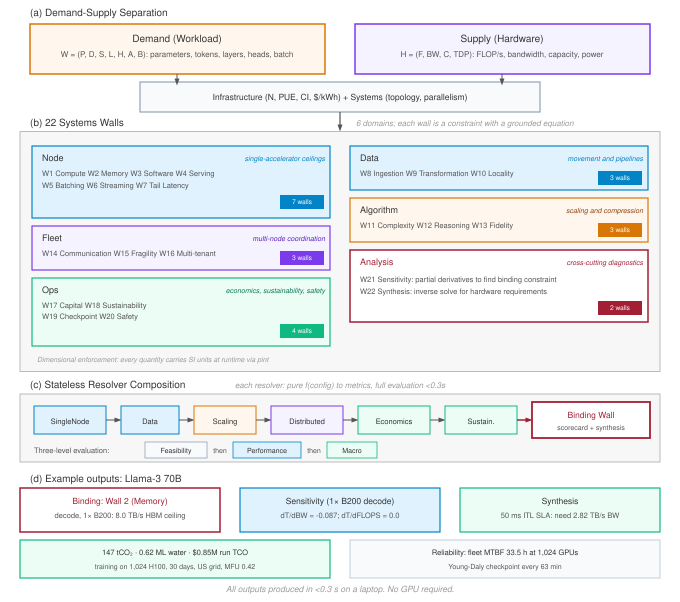
\includegraphics[width=\textwidth]{figures/mlsysim-overview.pdf}
\caption{\textbf{\mlsysim Framework Overview.} (a)~Demand--supply separation decouples workload specifications from hardware capabilities and environmental context. (b)~All \CountWalls{} Systems Walls organized into \CountDomains{} domains (Node, Data, Algorithm, Fleet, Operations, Analysis), each grounded in a published equation. (c)~Stateless resolver composition chains \CountResolvers{} resolvers to identify binding constraints through a three-level evaluation. (d)~Example outputs for Llama-3 70B: decode on one B200 (binding wall, sensitivities, and synthesized bandwidth) and a \OverviewDGpus-GPU H100 training fleet at MFU \OverviewDMfu{} (carbon, water, TCO, and reliability), all six solves completing in about \OverviewDSolveSeconds\,s on a laptop.}
\label{fig:overview}
\end{figure*}

\Cref{fig:overview} presents the end-to-end framework. This section unpacks the design in five parts. \Cref{sec:philosophy} introduces the four principles (analytical speed, dimensional strictness, taxonomic coverage, demand--supply separation) that constrain every subsequent decision. \Cref{sec:stack} translates those principles into a five-layer input stack of workloads, hardware, infrastructure, topology, and resolvers. \Cref{sec:types} describes the dimensionally strict type system that enforces correctness at every API boundary, \Cref{sec:extensibility} explains how new workloads, hardware, and resolvers compose with the existing pipeline without modification, and \Cref{sec:api} maps the public import surface and the presentation layer that sits outside the analytical engine.

\subsection{Design Philosophy}
\label{sec:philosophy}

The central question \mlsysim addresses is: \emph{Where does the complexity of an ML system come from?} We argue that complexity arises from the non-linear interaction of constraints across six distinct domains (node resources, data movement, algorithms, fleet coordination, operations, and cross-cutting analysis) and that an effective modeling tool must formalize \emph{all six} simultaneously. Four design principles govern \mlsysim's approach.

\subsubsection{Analytical Speed over Cycle Accuracy}
\label{sec:speed}

Analytical models that execute in sub-second time enable iterative design-space exploration that cycle-accurate simulators cannot support at comparable speed. By absorbing microarchitectural detail (cache hit rates, kernel scheduling) into a single efficiency parameter~$\eta$, \mlsysim achieves sub-second execution per solve. This enables sweeps over thousands of hardware--model--topology combinations in seconds, the kind of rapid ``what-if'' exploration that \citet{hennessy2024architecture} identify as necessary for quantitative architectural reasoning.

To maintain rigor despite analytical simplification, \mlsysim enforces a \textbf{``No Magic Numbers'' invariant}. Registry values carry a typed \texttt{Provenance} record whose \emph{kind} (datasheet, literature, industry report, convention, estimate, derived, illustrative, or heuristic) determines what evidence it must supply: evidence-backed kinds require a source URL and a verification date, while estimates and derived values require explanatory notes, and all records require a dated verification. The H100's FP16 rate is not a bare \texttt{989} floating-point literal; it is \texttt{989\,*\,TFLOPs\,/\,second}, half of the 1{,}979 teraFLOPS FP16 Tensor Core figure that NVIDIA publishes \emph{with sparsity}~\citep{nvidia2023h100}. Shared sources live once in a central catalog of \CountProvenanceRecords{} provenance records (\texttt{core.provenance\_catalog}) that registry entries reference by key, and an audit tool (\texttt{python -m mlsysim.tools.audit\_provenance}) walks every registry and fails on any value with missing or weak provenance. This discipline ensures that analytical speed does not come at the cost of reproducibility.

\subsubsection{Dimensional Strictness as an Invariant}
\label{sec:dimensional}

Dimensional consistency is a pervasive challenge in systems modeling. Mixing gigabits with gigabytes, or omitting the refractive index of fiber in latency calculations, are canonical failure modes that silently corrupt results. \mlsysim treats dimensional correctness not as a feature but as a \textbf{runtime invariant}, analogous to memory safety in Rust. The framework wraps every physical quantity using the \texttt{pint} unit library, and gives compute work its own base dimension: a FLOP is not a dimensionless count, so compute throughput can never silently add to, or convert into, a memory bandwidth. That confusion is the category error at the heart of many back-of-the-envelope mistakes. Mixing any two of \{compute rate, bandwidth, latency\} raises a deterministic \texttt{DimensionalityError} before any computation proceeds, while the ratios that \emph{should} compose still do: arithmetic intensity (FLOP/byte) divides cleanly, and utilization (achieved over peak FLOP rate) reduces to a dimensionless fraction:

\begin{lstlisting}[caption={\textbf{Dimensional Strictness.} Prevents silent unit errors at the API level.},label={lst:units}]
from mlsysim.core.units import Q_
rate = Q_("989 TFLOPs/s")    # Compute throughput
bw   = Q_("3.35 TB/s")       # Memory bandwidth
(rate / bw).to("flop/byte")  # -> 295 flop/byte (ridge point)
rate + bw  # -> raises DimensionalityError
\end{lstlisting}

This design eliminates the single most common class of bugs in back-of-the-envelope systems analysis, namely silent unit conversion errors.\footnote{The most infamous unit-conversion failure is the Mars Climate Orbiter, lost in 1999 because ground software produced thrust data in pound-force seconds while the spacecraft expected newton seconds~\citep{stephenson1999mco}.} Hardware and model specifications live in typed registries (e.g., \texttt{Hardware.Cloud.H100.memory.bandwidth = 3.35\,*\,TB/s}); the unit vocabulary lives in \texttt{core.units}, and physical constants and formulas live in \texttt{mlsysim.physics}, preventing unit mismatches at the API level. The physics formulas additionally validate the \emph{dimensionality} of their arguments, raising \texttt{DimensionalityError} when, for example, a byte count is passed where a bandwidth is expected.

\subsubsection{Taxonomic Coverage}
\label{sec:taxonomic}

We aim for broad coverage of the bottlenecks that have stable analytical formulations rather than for completeness, and \Cref{sec:discussion} lists the constraints we deliberately exclude. \mlsysim codifies 22 such bottlenecks, which we call \emph{Systems Walls}, organized into six domains: Node (single-accelerator resources), Data (movement and pipelines), Algorithm (scaling and compression), Fleet (multi-node coordination), Operations (economics, sustainability, and safety), and Analysis (cross-cutting diagnostics). Each wall maps to a resolver with a formal equation grounded in the systems literature. \Cref{sec:taxonomy} presents the full taxonomy with formal definitions, and \Cref{sec:solver-formalism} describes how solvers compose.

\subsubsection{Demand--Supply Separation}
\label{sec:demand-supply}

\mlsysim enforces a strict separation between \emph{what} a model computes and \emph{where} it runs. A \texttt{TransformerWorkload} describes computational demand (parameters, layers, FLOPs, arithmetic intensity) without reference to any specific accelerator. A \texttt{HardwareNode} describes physical supply (peak throughput, memory bandwidth, TDP) without reference to any specific model. This decoupling, inspired by the compiler IR philosophy of separating representation levels~\citep{hennessy2024architecture}, enables hardware--software co-design. The same GPT-3 workload can be evaluated against an H100, a TPU~v5p, or a hypothetical future accelerator in a single parametric sweep, with all dimensional conversions handled automatically.

\subsection{The Layered Input Stack}
\label{sec:stack}

\mlsysim implements these design principles through a five-layer architecture (\Cref{fig:stack}). Layers A--D are \emph{input layers} that describe demand, supply, context, and topology respectively. Layers A--C are independent of one another, and Layer~D composes Layer~B accelerators and, optionally, a Layer~C grid or datacenter into a fleet.  The single lowering step occurs in Layer~A, where a workload's \texttt{lower()} method produces a hardware-agnostic \texttt{ComputationGraph} intermediate representation.  Layer~E (Resolvers) then consumes any combination of layers A--D as needed; a single-node analysis requires only A+B, while a fleet-wide carbon estimate draws on A+B+C+D.

\begin{figure*}[!t]
\centering
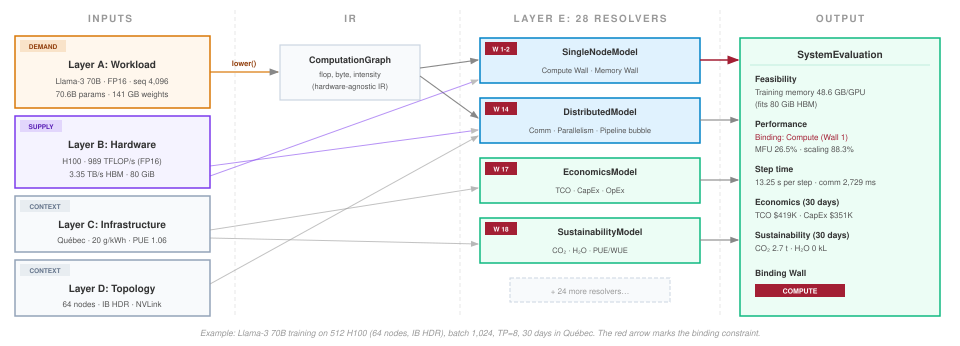
\includegraphics[width=\textwidth]{figures/architecture-stack.pdf}
\caption{\textbf{The \mlsysim 5-Layer Architecture.} Layers A--D provide typed inputs: workload demand, hardware supply, infrastructure context, and network topology. The single lowering step occurs in Layer~A, where \texttt{lower()} produces a hardware-agnostic Computation Graph (an intermediate representation of total FLOPs, weight bytes, and arithmetic intensity). Layer~E's \CountResolvers{} stateless resolvers consume these inputs and produce a three-level SystemEvaluation scorecard. The red arrow marks the binding constraint identified by the solver chain.}
\label{fig:stack}
\end{figure*}

\textbf{Layer A: Workloads (Demand).} A workload is a hardware-agnostic description of computational demand. \mlsysim provides five concrete workload types (\Cref{tab:workloads}), each exposing a \texttt{lower()} method that produces a \texttt{ComputationGraph} (an intermediate representation containing total operations, weight bytes, and arithmetic intensity in \texttt{flop/byte}). This IR is the contract between demand and supply, capturing \emph{what} must be computed without prescribing \emph{how}.

\begin{table}[!t]
\centering
\caption{\textbf{Supported Workload Types.} Each workload lowers to a \texttt{ComputationGraph} with total FLOPs, weight bytes, and arithmetic intensity.}
\label{tab:workloads}
\small
\renewcommand{\arraystretch}{1.1}
\begin{tabularx}{\columnwidth}{@{}l X l@{}}
\toprule
\textbf{Workload} & \textbf{Key Parameters} & \textbf{Scaling} \\
\midrule
Transformer     & $P$, $L$, $H$, $D$, seq.\ length & $2P$ FLOPs/token \\
CNN             & $P$, inference FLOPs             & Fixed per image \\
Sparse (MoE)    & Total vs.\ active $P$, experts   & Active $P$ for FLOPs \\
SSM (Mamba)     & $P$, state dim, $D$              & $O(1)$ state cache \\
Diffusion       & $P$, denoising steps $T$         & $T \times$ FLOPs/step \\
\bottomrule
\end{tabularx}
\end{table}

\textbf{Layer B: Hardware (Supply).} A \texttt{HardwareNode} composes four subsystems: \texttt{ComputeCore} (peak FLOP/s at the base FP16 precision plus a precision-keyed dictionary, e.g., TF32, FP8, INT8, FP32), \texttt{MemoryHierarchy} (capacity and bandwidth), optional \texttt{StorageHierarchy}, and optional \texttt{IOInterconnect}. Each node also carries TDP, unit cost, and a kernel dispatch tax. The \texttt{ridge\_point()} method computes the Roofline inflection $R = F_{\text{peak}} / BW_{\text{mem}}$ in \texttt{flop/byte}~\citep{williams2009}, enabling immediate classification of any lowered workload as compute-bound or memory-bound.

\textbf{Layer C: Infrastructure (Context).} \texttt{GridProfile} objects encode regional environmental parameters: carbon intensity (gCO$_2$/kWh), Power Usage Effectiveness (PUE), and Water Usage Effectiveness (WUE). A \texttt{Datacenter} composes a grid profile with an optional facility PUE override; rack power density is described separately by \texttt{RackProfile}. This layer converts raw energy consumption into carbon footprint and water usage, following the methodology of \citet{patterson2021carbon}.

\textbf{Layer D: Systems (Topology).} A \texttt{Fleet} composes \texttt{Node}s (each a physical compute server containing one or more accelerators on PCIe or NVLink) with a \texttt{NetworkFabric} (topology, inter-node bandwidth, latency, oversubscription ratio). This layer enables distributed analysis. The \texttt{DistributedModel} decomposes workloads using 4D parallelism (data-parallel~DP $\times$ tensor-parallel~TP $\times$ pipeline-parallel~PP $\times$ expert-parallel~EP) and calculates hierarchical AllReduce costs, pipeline bubble fractions, and scaling efficiency.

\textbf{Layer E: Resolvers (Analysis).} Twenty-eight stateless resolvers (23 models, 2 solvers, and 3 optimizers) consume demand, supply, context, and topology to produce dimensioned performance metrics. The solver formalism (stateless composition, chaining semantics, and three-level evaluation) is detailed in \Cref{sec:solver-formalism}.

The five layers are useful only if their inputs are reproducible. \mlsysim therefore organizes vetted specifications into eight curated registries collectively called the \emph{MLSys Zoo}: \textbf{Hardware} (accelerators and boards, plus technology classes under \texttt{Hardware.Tech}), \textbf{Models} (workload architectures across six family files: language, vision, generative vision, recommendation, state-space, and TinyML), \textbf{Datasets} (benchmark catalog entries), \textbf{Platforms} (deployment envelopes), \textbf{Infrastructure} (grids, datacenters, racks, cooling, pricing, and capacity), \textbf{Systems} (nodes, racks, fabrics, clusters, pods, and storage paths), \textbf{Ops} (operational policies and overhead profiles such as training-run goodput budgets and monitoring thresholds), and executable \textbf{Scenarios} that compose existing model, hardware, infrastructure, and system entries with local constraints such as latency, power, run length, or region without redefining the underlying facts. Two extension registries, \textbf{Agents} (agentic workload profiles) and \textbf{Embodied} (robot platforms), sit outside the wall taxonomy; \Cref{sec:discussion} explains why. Two auxiliary surfaces complete the picture: non-executable real-world anchors, such as Waymo data-rate ranges or mobile power envelopes, live in \texttt{ReferenceStats.*}, and cited field figures (MFU bands, scaling laws) live in \texttt{Literature.*}. Solver fallbacks live in \texttt{mlsysim.engine.calibration}; architecture formulas (Roofline, AllReduce, Young--Daly) live in \texttt{mlsysim.physics}; the machine-readable wall taxonomy of \Cref{tab:walls} ships as \texttt{mlsysim.engine.walls}; and domain-reviewed empirical anchors in \texttt{mlsysim.engine.empirical} bind registry entries to published benchmark envelopes for regression testing.

Registry entries are authored as YAML data files and validated against \texttt{pydantic} schemas at import time, so stating a fact is a data edit while computing or composing remains Python. The loader rejects duplicate keys outright and resolves two reference forms: \texttt{@tech:} pointers that let an instance inherit a technology-class fact, and \texttt{@prov:} pointers into the shared provenance catalog (\Cref{sec:speed}). The \texttt{Hardware.Tech} sub-registry encodes the load-bearing distinction between \emph{instances} and \emph{technology classes}: per-part facts that vary between products (capacity, bandwidth, TDP, price) live on instances such as \texttt{Hardware.Cloud.H100}, while facts that are properties of a technology generation (access latency, energy per operation, interconnect latency) live once on tech-class entries. For example, \texttt{Hardware.Cloud.H100} takes its NVLink latency from \texttt{Hardware.Tech.Interconnect.NVLink} through an \texttt{@tech:} reference, and instance lookups fall back to the tech class when a value is unset. Each registry entry is a fully typed object; for example, \texttt{Hardware.Cloud.H100} returns a \texttt{HardwareNode} with all physical quantities dimensioned via \texttt{pint}. \Cref{fig:registry-composition} illustrates how these reusable facts become a concrete infrastructure model: a scenario binds a workload, accelerator fleet, regional grid, and operational policy to a local question, then passes the resulting typed objects to the resolver chain.

\begin{figure*}[!t]
\centering
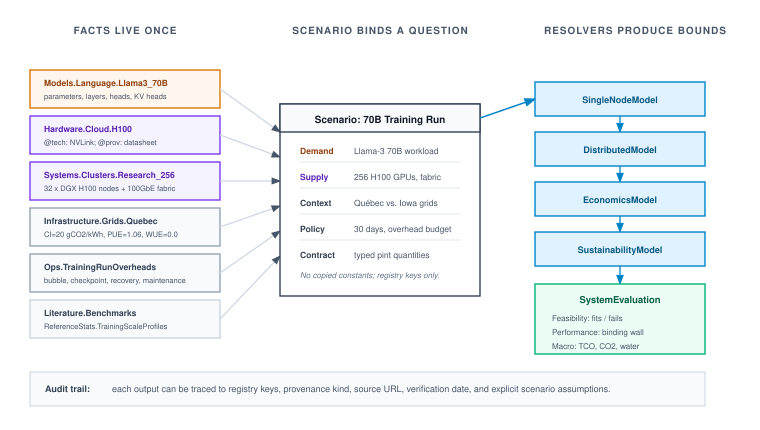
\includegraphics[width=\textwidth]{figures/registry-composition.pdf}
\caption{\textbf{Registry-Backed System Composition.} \mlsysim stores workload, hardware, systems, infrastructure, operational, and literature facts once, with typed schemas and provenance records. A scenario composes those reusable facts into a local infrastructure question---for example, training a 70B model on a 256-GPU H100 fleet in Qu\'ebec or Iowa---and hands dimensioned objects to the resolver chain. The resulting \texttt{SystemEvaluation} can be traced back to the registry keys, source records, and scenario assumptions that produced it.}
\label{fig:registry-composition}
\end{figure*}

Once a scenario has assembled typed inputs, the \texttt{physics} package decomposes the framework's analytical equations into eleven domain-aligned modules (\Cref{tab:physics-modules}), each owning one conceptual domain of the systems stack, plus two supporting modules: \texttt{physics.constants} holds universal physical constants (e.g., the speed of light in fiber), and \texttt{physics.quantities} provides generic dimensioned helpers (transfer time, compute time, energy from power, carbon from energy). A shared \texttt{\_ensure\_unit()} helper coerces raw floats into \texttt{pint} quantities at module entry points, guaranteeing dimensional correctness without burdening callers. Chapter and notebook code import from \texttt{mlsysim.physics} directly. The appendix (\Cref{tab:physics-api}) lists representative function signatures.

\begin{table}[!t]
\centering
\caption{\textbf{Physics Domain Modules.} Each module owns the analytical formulas for one domain. The two extension modules sit outside the wall taxonomy (\Cref{sec:discussion}).}
\label{tab:physics-modules}
\small
\renewcommand{\arraystretch}{1.08}
\begin{tabularx}{\columnwidth}{@{}l l X@{}}
\toprule
\textbf{Module} & \textbf{Domain} & \textbf{Key Formulas} \\
\midrule
\texttt{performance}    & Node        & Roofline bottleneck, Amdahl's speedup, pipeline bubble \\
\texttt{memory}         & Node        & Model memory, activation memory, KV-cache, checkpoint size \\
\texttt{serving}        & Node        & Erlang-C M/M/$c$ queue latency \\
\texttt{communication}  & Fleet       & Ring/tree/hierarchical AllReduce, All-to-All \\
\texttt{reliability}    & Fleet       & Young--Daly, cluster MTBF, failure probability \\
\texttt{transformer}    & Algorithm   & Training/decode FLOP counts \\
\texttt{economics}      & Operations  & Fleet TCO, egress cost \\
\texttt{networking}     & Data        & Speed-of-light latency \\
\texttt{statistics}     & Analysis    & PSI drift detection, sample sizing \\
\midrule
\texttt{agents}         & Extension   & Trajectory reliability, test-time compute cost, multi-agent coordination \\
\texttt{robotics}       & Extension   & Sensor-to-actuator latency, safe stopping distance, action-chunk cadence \\
\bottomrule
\end{tabularx}
\end{table}

The \textbf{Hardware} registry holds \CountHardwareDevices{} devices across five deployment tiers (Cloud, Workstation, Edge, Mobile, Tiny), spanning nine orders of magnitude in peak throughput from milliwatt-class microcontrollers (\texttt{Hardware.Tiny.ESP32\_S3}, 520\,KiB on-chip SRAM) to wafer-scale engines (\texttt{Hardware.Cloud.Cerebras\_CS3}, 44\,GB on-wafer SRAM, 125\,PFLOP/s). Beyond NVIDIA GPUs (T4 and V100 through B200 and the rack-scale GB200~NVL72), the registry includes AMD MI250X and MI300X, Intel Gaudi~2 and Gaudi~3, AWS Trainium~2, and the full Google TPU lineage (v1 through v6/Trillium), enabling cross-vendor design-space exploration, plus workstation (Apple M3 Max, DGX Spark), edge (Jetson, Coral), mobile (Apple A17 Pro, Snapdragon 8 Gen~3, Tensor G3), and TinyML (ESP32-S3, nRF52840, Himax WE-I Plus) devices. The \texttt{list(sort\_by=)} class method enables programmatic comparison, and users extend any zoo by instantiating new typed objects (\Cref{lst:hwnode}) or adding YAML data files, ensuring custom entries participate in the same dimensionally strict pipeline as vetted ones. \Cref{fig:anatomy} maps the implementation structure behind this composition path: panel~(a) shows package architecture (registries, physics modules, core utilities, and invariant checks), while panel~(b) traces a concrete analysis from typed inputs through the resolver chain to the three-level \texttt{SystemEvaluation} scorecard. \Cref{sec:appendix-hardware} gives a representative snapshot of the current registry surface.

\begin{figure*}[!t]
\centering
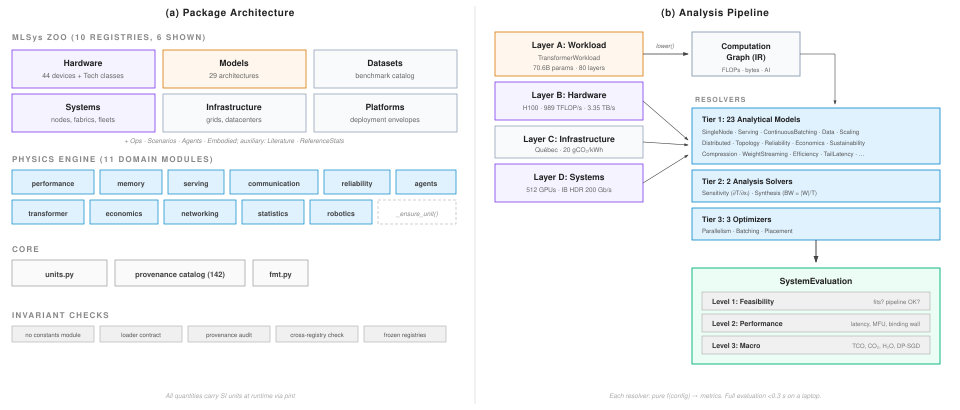
\includegraphics[width=\textwidth]{figures/system-anatomy.pdf}
\caption{\textbf{System Anatomy.} (a)~Package architecture: \CountRegistriesCurated{} curated registries (six shown) provide typed, provenance-tracked specifications, \CountPhysicsDomainModules{} domain physics modules supply the formulas, and five invariant checks enforce design decisions as the codebase evolves. (b)~Analysis pipeline: a workload lowers to a hardware-agnostic intermediate representation; four input layers feed \CountResolvers{} stateless resolvers organized in three tiers; the output is a three-level \texttt{SystemEvaluation} scorecard (Feasibility, Performance, Macro).}
\label{fig:anatomy}
\end{figure*}

\subsection{The Type System}
\label{sec:types}

\mlsysim's type system is built on Pydantic \texttt{BaseModel} classes with \texttt{pint} \texttt{Quantity} fields, providing both schema validation and dimensional enforcement at construction time. The same schemas validate the YAML registry data: every \texttt{*.yaml} entry is instantiated through its \texttt{pydantic} type at import, so a malformed unit string fails the import rather than surfacing later as a wrong number, and a missing provenance record fails the provenance audit. The composition hierarchy is deliberately shallow: \texttt{HardwareNode} aggregates \texttt{ComputeCore} and \texttt{MemoryHierarchy} as direct fields, not through deep inheritance. This design makes the relationship between a hardware specification and its physical quantities immediately legible:

\begin{lstlisting}[caption={\textbf{Custom Hardware Node.} Composing a hardware specification with dimensional types.},label={lst:hwnode}]
from mlsysim.hardware.types import *
from mlsysim.core.units import Q_
node = HardwareNode(
    name="Custom Accelerator",
    release_year=2025,
    compute=ComputeCore(
        peak_flops=Q_("500 TFLOPs/s"),
        precision_flops={"fp8": Q_("1000 TFLOPs/s")}),
    memory=MemoryHierarchy(
        capacity=Q_("96 GiB"),
        bandwidth=Q_("4 TB/s")),
    tdp=Q_("500 W"))
print(node.ridge_point())  # -> 125.0 flop/B
\end{lstlisting}

The \texttt{ComputationGraph} IR bridges the demand--supply gap. When a solver calls \texttt{workload.lower()}, the workload computes its total operations, weight bytes, and arithmetic intensity, all in dimensioned quantities. For Mixture-of-Experts models, \texttt{SparseTransformerWorkload.lower()} uses \emph{active} parameters for FLOPs but \emph{total} parameters for memory footprint, correctly modeling the fundamental decoupling between compute cost and capacity requirements in sparse architectures~\citep{shazeer2017outrageously}.

The evaluation produces a \texttt{SystemEvaluation} scorecard that groups the metrics of the composed resolvers into Feasibility, Performance, and Macro levels. Students can inspect any individual level or view the aggregate to understand how constraints interact across the stack.

\subsection{Extensibility}
\label{sec:extensibility}

The layered architecture is designed for extension at every level. New workload types (e.g., a \texttt{RetrievalAugmentedWorkload} for RAG pipelines) require implementing the \texttt{lower()} method to produce a \texttt{ComputationGraph}. Resolvers that consume only the graph, such as the \texttt{SingleNodeModel}, then apply unchanged, while architecture-specific resolvers such as the \texttt{ServingModel} also require transformer fields. New hardware entries are added to the \textbf{Hardware} registry as declarative \texttt{HardwareNode} specifications (\Cref{lst:hwnode}), with no resolver changes needed. New resolvers can be introduced for emerging constraints by implementing the appropriate tier interface: a Tier 1 Model (e.g., a \texttt{PrivacyModel} for federated learning overhead), a Tier 2 Solver, or a Tier 3 Optimizer.

By accepting typed inputs and returning dimensioned outputs, the type system enforces correctness at every boundary, ensuring that custom extensions compose safely with existing components. This design ensures that \mlsysim can track the rapidly evolving ML systems landscape without requiring architectural changes to the core framework.

\subsection{Public API and Presentation Layer}
\label{sec:api}

The package separates analysis from presentation. \texttt{from mlsysim import *} exposes the registries, the physics formulas, the unit vocabulary, and the formatting helpers; solver classes are imported through the stable \texttt{mlsysim.solvers} path, which mechanically re-exports the canonical implementations in \texttt{mlsysim.engine.solvers} so the two surfaces cannot drift. The \texttt{engine} package is the infrastructure-modeling core: the Roofline core (\texttt{engine.engine}), the 28 resolvers, the three-level evaluation, pipeline composition, design-space exploration, executable scenarios, the machine-readable wall taxonomy, calibration defaults, and empirical anchors. Presentation lives outside the engine: \texttt{mlsysim.fmt} provides a typed \texttt{fmt\_*} formatter family (50+ helpers for quantities, counts, currencies, percentages, and scientific notation) whose outputs are Markdown-safe strings and whose precision-safety guards refuse to render non-finite values or to silently round a non-zero value to the literal ``0''; \texttt{mlsysim.viz} supplies matplotlib plotters with a consistent style; and a command-line interface (\texttt{python -m mlsysim}) exposes the zoo browser, scenario evaluation, serving analysis, design-space optimization, a local-hardware Iron Law audit, and schema export.

% ============================================================
\section{Taxonomy of ML Systems Walls}
\label{sec:taxonomy}

\begin{table}[!t]
\centering
\caption{\textbf{Notation.} Symbols used throughout; all quantities carry SI units at runtime via \texttt{pint}.}
\label{tab:notation}
\footnotesize
\setlength{\tabcolsep}{4pt}
\renewcommand{\arraystretch}{1.05}
\begin{tabularx}{\columnwidth}{@{}l l X@{}}
\toprule
\textbf{Symbol} & \textbf{Unit} & \textbf{Description} \\
\midrule
\multicolumn{3}{@{}l}{\textit{Model \& Workload}} \\
$P$, $P_{\ell}$ & params & Total / per-layer parameter count \\
$|W|$, $|W_{\ell}|$ & bytes & Bytes read per step / per layer \\
$b_{\text{prec}}$ & B/param & Precision (e.g., 2 for FP16) \\
$L$, $H$, $D$ & -- & Layers, attention heads, head dim \\
$S$ & tokens & Sequence length \\
$B$ & samples & Batch size \\
$K$ & -- & Reasoning steps \\
$C$ & FLOPs & Training compute ($6PD$) \\
$I$ & FLOP/B & Arithmetic intensity \\
\midrule
\multicolumn{3}{@{}l}{\textit{Hardware \& Infrastructure}} \\
$\text{Peak}_{\text{FLOPS}}$ & FLOP/s & Peak accelerator throughput \\
$BW_{\text{HBM}}$ & B/s & HBM bandwidth \\
$BW_{\text{inject}}$ & B/s & Injection BW (wafer-scale) \\
$BW_{\text{link}}$ & B/s & Per-link network bandwidth \\
$N$, $G$ & -- & Nodes in fleet, GPUs per node \\
$\alpha$ & s & Per-hop network latency \\
\midrule
\multicolumn{3}{@{}l}{\textit{Efficiency \& Utilization}} \\
$\eta$ & -- & HW utilization ($\approx$ MFU) \\
$\eta_{\text{overlap}}$ & -- & Compute--comm overlap \\
$\rho$ & -- & Utilization ratio (queue/data) \\
$\beta$, $\beta_{\text{opt}}$ & -- & Bisection BW frac, optimizer multiplier \\
\midrule
\multicolumn{3}{@{}l}{\textit{Parallelism}} \\
TP, PP, DP, EP & -- & Tensor, pipeline, data, expert parallel \\
$V$, $M_{\text{micro}}$ & -- & Virtual stages, microbatches \\
\midrule
\multicolumn{3}{@{}l}{\textit{Sustainability}} \\
PUE, WUE & --, L/kWh & Power / Water Usage Effectiveness \\
$\text{CI}$ & gCO$_2$/kWh & Regional carbon intensity \\
\midrule
\multicolumn{3}{@{}l}{\textit{Key Derived Quantities}} \\
$I^{*}$ & FLOP/B & Ridge point ($\text{Peak}/BW_{\text{HBM}}$) \\
$B^{*}$, $P^{*}$, $D^{*}$ & varies & Optimal batch, model, dataset size \\
$\tau_{\text{opt}}$ & s & Optimal checkpoint interval \\
\bottomrule
\end{tabularx}
\end{table}

The ML systems literature is rich with specialized models for specific bottlenecks, from the original Roofline model~\citep{williams2009} and Chinchilla scaling laws~\citep{hoffmann2022chinchilla} to PagedAttention batching limits~\citep{kwon2023} and datacenter sustainability accounting~\citep{patterson2021carbon}. However, these constraints are typically studied in isolation. We synthesize this disjointed literature into a unified taxonomy of 20 distinct ``Walls'' plus 2 cross-cutting diagnostic tools (Sensitivity and Synthesis). We borrow the term from the computer architecture tradition (the ``memory wall''~\citep{wulf1995memorywall}, the ``power wall''~\citep{hennessy2024architecture}), where a \emph{wall} denotes a hard physical or logical constraint that bounds system performance. Codifying these previously disparate equations into a single, composable framework, each wall maps to a resolver (model or solver) that accepts typed inputs and produces dimensionally correct bounds. We are not aware of a prior tool that integrates these constraints in one executable engine. The complete taxonomy is summarized in \Cref{tab:walls}.

The taxonomy proceeds outward from the silicon. \Cref{sec:walls-node} covers the seven Node walls that bound a single accelerator (compute, memory, software efficiency, serving, batching, streaming, tail latency). \Cref{sec:walls-data} adds the three Data walls that govern how samples reach the accelerator (ingestion, transformation, locality). \Cref{sec:walls-algorithm} covers the three Algorithm walls that originate in the mathematics of learning (complexity, reasoning, fidelity). \Cref{sec:walls-fleet} adds the three Fleet walls that arise once a job spans multiple nodes (communication, fragility, multi-tenant scheduling). \Cref{sec:walls-operations} covers the four Operations walls that determine whether a system should run at all (capital, sustainability, checkpoint, safety). Finally, \Cref{sec:walls-analysis} introduces the two cross-cutting diagnostic tools (Sensitivity and Synthesis) that operate across the entire taxonomy.

\subsection{Node (Single-Accelerator Resources)}
\label{sec:walls-node}

The Node walls define what a single accelerator (one physical processing unit such as a GPU, TPU, or wafer-scale engine, used interchangeably with ``individual accelerator'') can achieve in isolation, before any distributed coordination is considered. Multi-node analysis, where a server hosts several such accelerators on intra-node links such as NVLink, falls under the Fleet domain (\Cref{sec:walls-fleet}). Node walls are the innermost constraints and the first a practitioner should evaluate.

\textbf{Wall~1: The Compute Wall.} Every accelerator has a hard throughput ceiling determined by the number of arithmetic units and the clock frequency. An H100, for example, provides a peak of \cvalint{\HhPeakTFLOPS}\,TFLOP/s at FP16 with Tensor Cores, establishing an upper bound that no software optimization can exceed. The \texttt{SingleNodeModel} evaluates the classical Roofline model bounds~\citep{williams2009}. If execution is entirely compute-bound, the minimum time to process the workload is dictated by the \emph{Iron Law of ML Systems}:
\begin{equation}
\label{eq:tcompute}
T_{\text{compute}} = \frac{\text{OPs}}{\text{Peak}_{\text{FLOPS}} \times \eta}
\end{equation}
where $\eta \in (0,1]$ is the hardware utilization efficiency and OPs is the total operation count. Throughout this paper, $\eta$ denotes the ratio of sustained to peak throughput; the related metric \emph{Model FLOPS Utilization} (MFU) measures only model-useful FLOPs and excludes overhead such as activation recomputation. For first-order analysis, we treat $\eta \approx \text{MFU}$; the distinction matters only when recomputation or non-model compute is significant. When this wall binds, the only remedy is faster silicon or fewer operations. \textbf{Assumptions:} Peak FLOPS is a hard ceiling; $\eta$ is workload-dependent and must be specified or estimated from benchmark data.

\textbf{Wall~2: The Memory Wall.} High-bandwidth memory (HBM) imposes two ceilings: capacity (the model must fit) and bandwidth (weights must stream to compute units fast enough). An H100 reads HBM at \cvalii{\HhBWTBs}\,TB/s, yet its \cvalint{\HhPeakTFLOPS}\,TFLOP/s demand data at a rate that exceeds this bandwidth for any workload below ${\sim}\cvalint{\HhRidgePoint}$\,flop/byte, making most LLM inference memory-bound, not compute-bound. During training, techniques like \textbf{Low-Rank Adaptation (LoRA)} and \textbf{Activation Recomputation} fundamentally alter the capacity constraint by trading compute or parameter trainability for drastically reduced memory footprints. The same \texttt{SingleNodeModel} computes~\citep{williams2009}:
\begin{equation}
\label{eq:tmemory}
T_{\text{memory}} = \frac{|W|}{BW_{\text{HBM}}}
\end{equation}
where $|W|$ is the total bytes read per inference step. The realized execution time is the maximum of the two bounds:
\begin{equation}
\label{eq:bottleneck}
T = \max(T_{\text{compute}},\; T_{\text{memory}})
\end{equation}
The crossover between compute-bound and memory-bound regimes occurs at the \emph{ridge point}, the arithmetic intensity at which the two ceilings intersect:
\begin{equation}
\label{eq:ridge}
I^{*} = \frac{\text{Peak}_{\text{FLOPS}}}{BW_{\text{HBM}}} \quad \text{(flop/byte)}
\end{equation}
Workloads with arithmetic intensity $I < I^{*}$ are memory-bound; those with $I > I^{*}$ are compute-bound. \textbf{Assumptions:} Peak FLOPS and HBM bandwidth are hard ceilings; MFU accounts for software inefficiency via $\eta$.

For training, capacity pressure is larger than inference weight residency alone. The \texttt{TrainingMemoryModel} exposes the first-order per-accelerator accounting directly:
\begin{equation}
\label{eq:training-memory}
M_{\text{train}} =
M_{\text{weights}} + M_{\text{grad}} + M_{\text{opt}} +
M_{\text{act}} + M_{\text{comm}}.
\end{equation}
Mixed-precision Adam defaults to FP16/BF16 weights and gradients plus FP32 master weights and optimizer moments, while tensor, pipeline, expert, and ZeRO sharding reduce different terms of the sum~\citep{shoeybi2019megatron,rajbhandari2020}. Activation checkpointing reduces $M_{\text{act}}$ by recomputing intermediate tensors during backward pass; the activation term implements the per-layer analytical bounds of \citet{korthikanti2023} ($34\,sbh$ bytes per layer with selective recomputation; $34\,sbh + 5as^2b$ without, where $s$, $b$, $h$, $a$ are sequence length, microbatch size, hidden dimension, and attention heads). The model intentionally reports each term separately so students can see whether a configuration fails because of optimizer state, activations, or communication buffers rather than a generic ``out of memory'' label.

\textbf{Wall~3: The Software Wall.} The gap between peak and achieved FLOP/s is typically larger than the gap between hardware generations. Megatron-LM's single-V100 baseline sustained only 30\% of theoretical peak FLOPs~\citep{shoeybi2019megatron}, and published MFU for large training runs spans 21.3\% to 46.2\%~\citep{chowdhery2022palm}; much of the gap comes from memory traffic, idle kernels, and unfused operations. The \texttt{EfficiencyModel} models this as a multiplicative efficiency factor:
\begin{equation}
\label{eq:efficiency}
\eta = \frac{\text{FLOPS}_{\text{achieved}}}{\text{Peak}_{\text{FLOPS}}}
\end{equation}
where $\eta \in (0,1]$ modulates the Roofline ceiling, reducing the effective peak from $\text{Peak}_{\text{FLOPS}}$ to $\eta \times \text{Peak}_{\text{FLOPS}}$. FlashAttention~\citep{dao2022}, for example, reports a $3\times$ end-to-end training speedup on GPT-2 at sequence length 1K by fusing attention into IO-aware kernels that cut HBM reads and writes; the \texttt{EfficiencyModel} represents this kind of gain by raising attention-layer $\eta$ from 0.3 to an illustrative 0.75. When this wall binds, better kernels, not bigger chips, are the remedy. \textbf{Assumption:} $\eta$ is a single scalar that aggregates all software inefficiencies; in practice, different operations (GEMM vs.\ attention vs.\ normalization) achieve different utilization on the same silicon. To avoid circularity when $\eta$ is unknown, the \texttt{EfficiencyModel} draws its defaults from the registry's literature bounds for large-scale training, $\eta = 0.30$ to $0.50$, consistent with published MFU~\citep{chowdhery2022palm,llama3team2024}. At its default setting, attention layers get the lower bound, FFN layers the upper bound (capped at 0.60), and convolutions the midpoint (capped at 0.55). Students can use these defaults as starting points and refine as they gather profiling data.

\textbf{Wall~4: The Serving Wall.} Autoregressive LLM inference exhibits two distinct phases with fundamentally different Roofline characteristics~\citep{pope2023llm}. For a 70B model on two tensor-parallel H100s, a \cvalint{\ServSin}-token prefill takes ${\sim}\cvalint{\ServPrefillMs}$\,ms (compute-bound) while each decode token costs ${\sim}\cvalint{\ServDecodeMs}$\,ms (memory-bound). Prefill processes all input tokens in parallel (${\sim}\cvalint{\ServPrefillTps}$ tokens/s), while decode generates one token per memory-bandwidth pass (${\sim}\cvalint{\ServDecodeTps}$ tokens/s), a ${\sim}\cvalint{\ServTpsRatio}{\times}$ throughput gap. The \texttt{ServingModel} decomposes end-to-end inference latency as:
\begin{align}
\label{eq:serving}
T_{\text{prefill}} &= \frac{2P \cdot S_{\text{in}}}{\text{Peak}_{\text{FLOPS}} \times \eta} \quad \text{(compute-bound)} \\
T_{\text{decode}} &= \frac{|W|}{BW_{\text{HBM}}} \quad \text{(memory-bound)}
\end{align}
where $S_{\text{in}}$ is the input sequence length, $P$ is the parameter count, and $|W|$ includes both model weights and KV-cache reads (which grow with batch size and context length: $|W| = |W_{\text{model}}| + |W_{\text{KV}}|$). The $2PS$ term accounts for the linear projection FLOPs. The self-attention computation adds $\mathcal{O}(S^2)$ FLOPs per layer; under the \texttt{ServingModel} FLOP accounting it is \WallFourAttnShareEightKPct\% of prefill FLOPs for Llama-3 70B at \WallFourAttnSeqShort{} tokens and \WallFourAttnShareThirtyTwoKPct\% at \WallFourAttnSeqLong{}. The \texttt{ServingModel} includes this attention term explicitly. When serving multiple concurrent requests ($B > 1$), model weights are loaded from HBM once per step while KV-cache reads grow linearly with the batch: $T_{\text{step}} = (|W| + B \cdot |KV_1|) / BW$, where $|KV_1|$ is the per-request KV-cache size. Because each step produces $B$ tokens simultaneously, the effective per-token cost is $T_{\text{step}}/B$, amortizing the weight read across requests. At large batch sizes the per-request KV cache dominates and throughput saturates.

The model also exposes an optional chunked-prefill estimate inspired by Sarathi-Serve~\citep{agrawal2025}. When \texttt{prefill\_chunk\_tokens} is set, only the new, uncached prefill work is partitioned into chunks:
\begin{align}
\label{eq:chunked-prefill}
C_{\text{prefill}} &=
\max\!\left(1,\left\lceil\frac{S_{\text{in}} - S_{\text{cache}}}{S_{\text{chunk}}}\right\rceil\right), \\
T_{\text{stall}} &= \max_i\left(T_{\text{chunk},i}\right)
\end{align}
where $T_{\text{chunk},i}$ is the compute time for chunk $i$ plus one dispatch tax. The resulting \texttt{ServingResult} reports \texttt{prefill\_chunks} ($C_{\text{prefill}}$), \texttt{prefill\_chunk\_time} ($T_{\text{stall}}$), and \texttt{decode\_stall\_bound}, which is set to $T_{\text{stall}}$ as a first-order bound on how long the slowest prefill chunk can interfere with ongoing decode iterations. This is a coarse analytical bound, not a full scheduler: total TTFT still includes the same prefill compute work plus one dispatch tax per chunk, and the solver does not claim Sarathi-Serve's stall-free packing behavior.

For deployment sizing, the serving-capacity resolver combines serving latency, continuous-batching capacity, and tail-queueing estimates. Given average generated length $G$ and per-replica token throughput $R_{\text{tok}}$, it estimates request capacity as
\begin{align}
\label{eq:serving-capacity}
Q_{\text{replica}} &= \frac{R_{\text{tok}}}{G}, \\
P99_{\text{request}} &\approx T_{\text{base}} + P99_{\text{queue}} \le T_{\text{target}}.
\end{align}
This converts a common serving question---``how many replicas do I need for a QPS and P99 target?''---into a transparent composition of the latency, batching, and queueing walls. The compute efficiency $\eta$ remains an exposed parameter with the same interpretation as in the Roofline model; the default is a starting point, not a claim of universal serving efficiency.

The prefill phase processes all input tokens in parallel and is compute-bound; the decode phase generates one token at a time and is memory-bandwidth-bound. The solver incorporates modern paradigms including \textbf{Prompt Caching} (prefix caching~\citep{zheng2024sglang}, which reduces TTFT by skipping prefill for previously computed KV-cache entries), \textbf{Speculative Decoding} (probability-weighted verification using a smaller draft model~\citep{leviathan2023fast}), \textbf{Disaggregated Serving} (phase splitting onto different hardware with KV-cache network transfer~\citep{patel2024}), and \textbf{Chunked Prefill} (optional chunk-level stall bounds for interleaving prefill work with decode~\citep{agrawal2025}). This duality explains why batching strategies that improve prefill throughput may have no effect on decode latency, because the two phases are bound by different resources. \textbf{Assumptions:} Prefill is compute-bound for sequence lengths $S_{\text{in}} \gg 1$; decode is memory-bandwidth-bound at batch size 1. Chunked prefill partitions the same upper-bound prefill work by token count with a fixed dispatch tax per chunk, so \texttt{decode\_stall\_bound} is a scheduling proxy rather than a measured tail-latency guarantee. At large batch sizes decode compute grows with the batch and can approach the compute ceiling. The \texttt{ServingModel} does not model this crossover, because its decode time is the memory-bound term alone; the \texttt{SingleNodeModel} Roofline shows which ceiling binds.

\textbf{Wall~5: The Batching Wall.} Decode is memory-bound, so the number of requests that share a decode step is the main throughput lever, and the KV-cache allocator decides how many requests fit. A static allocator reserves a contiguous slot of $S_{\max}$ tokens for every request, whatever length the request actually reaches. A paged allocator, as in PagedAttention~\citep{kwon2023}, divides the KV budget into blocks of $p$ tokens and gives a request of $S$ tokens $\lceil S/p \rceil$ blocks on demand. With $M_{\text{KV}}$ the HBM left after the weights and $k$ the KV bytes per token, the \texttt{ContinuousBatchingModel} computes the concurrency each allocator admits:
\begin{equation}
\label{eq:pagedkv}
N_{\text{static}} = \left\lfloor \frac{M_{\text{KV}}}{k\,S_{\max}} \right\rfloor, \qquad
N_{\text{paged}} = \left\lfloor \frac{\lfloor M_{\text{KV}}/(k\,p) \rfloor}{\mathbb{E}\left[\lceil S/p \rceil\right]} \right\rfloor
\end{equation}
where request lengths are exponential with mean $\bar{S}$ and cut off at $S_{\max}$, and the scheduler's maximum batch size caps both counts. The unused share of each allocation is $1 - \bar{S}/S_{\max}$ under static reservation and about one partially filled block per request under paging. Memory-bound decode reads the weights once per step plus the tokens that requests have filled, so $t_{\text{step}} = (|W| + N\bar{S}k)/BW_{\text{HBM}}$ and token throughput is $N/t_{\text{step}}$. For Llama-3 8B on an H100 with $S_{\max} = \WallFiveMaxSeqLen$ and $\bar{S} = \WallFiveMeanTokens$, static reservation admits \WallFiveStaticUsers{} requests and leaves \WallFiveStaticWastePct\% of each reservation unused, while \WallFivePageSize-token pages admit \WallFivePagedUsers{} requests with \WallFivePagedWastePct\% unused, a $\WallFiveSpeedup{\times}$ gain in decode throughput; \WallFiveLargePageSize-token pages admit only \WallFiveLargePagePagedUsers{}. Kwon et al.\ profile contiguous pre-allocation and find that only 20.4\% to 38.2\% of KV-cache memory holds token states, with the remainder lost to reserved slots, internal fragmentation, and external fragmentation, whereas vLLM reaches 96.3\%~\citep{kwon2023}. \textbf{Assumptions:} Request lengths are exponential, and every admitted request is sized at its full length (peak occupancy), which makes paged capacity conservative. The static baseline is max-length reservation with no external fragmentation; exact-size and power-of-two contiguous allocators are not modeled. When the batch-size cap binds both allocators, allocation policy does not change throughput.

\textbf{Wall~6: The Streaming Wall.} Wafer-scale architectures~\citep{lie2022cerebras} (e.g., Cerebras CS-3) invert the conventional memory hierarchy. Activations reside on-wafer in SRAM while model weights stream from external MemoryX nodes, shifting the bottleneck from HBM bandwidth to injection interconnect bandwidth. The \texttt{WeightStreamingModel} models this as:
\begin{equation}
\label{eq:weightstream}
T_{\text{layer}} = \max\!\left(\frac{|W_{\ell}|}{BW_{\text{inject}}},\; \frac{2P_{\ell} \times B}{\text{Peak} \times \eta}\right)
\end{equation}
where $|W_{\ell}|$ is the layer weight size in bytes, $P_{\ell} = |W_{\ell}| / b_{\text{prec}}$ is the parameter count (with $b_{\text{prec}}$ bytes per element), and the factor of 2 accounts for the multiply-accumulate FLOPs per parameter. The two terms inside the $\max$ represent the injection time (weight delivery) and the compute time (matrix arithmetic) for one layer. When $B$ is small, weight injection dominates and the compute engine sits idle; when $B$ is large, compute dominates and the injection link sits idle. Setting the two terms equal and substituting $|W_{\ell}| = P_{\ell} \times b_{\text{prec}}$ yields the optimal batch size $B^{*} = (b_{\text{prec}} \times \text{Peak} \times \eta) / (2 \times BW_{\text{inject}})$. This result depends only on numerical precision, peak compute, and injection bandwidth, independent of layer size. This is the unique operating point where injection and compute perfectly overlap, maximizing utilization of both resources. \textbf{Assumptions:} Layer weights dominate the injection payload; 10\% overhead is reserved for working memory; perfect within-layer pipelining is assumed.

\textbf{Wall~7: The Tail Latency Wall.} At scale, P99 latency governs user experience, not the median. Fan-out compounds the tail: if a request must collect responses from 100 servers whose 99th-percentile latency is one second, 63\% of such requests take more than one second~\citep{dean2013}. The \texttt{TailLatencyModel} models inference replicas as an M/M/$c$ queue using the Erlang-C formula~\citep{harcholbalter2013}:
\begin{equation}
\label{eq:erlangc}
\mathbb{P}[\text{wait}] = \frac{(c\rho)^c / c! \cdot (1-\rho)^{-1}}{\sum_{k=0}^{c-1}(c\rho)^k/k! + (c\rho)^c/c! \cdot (1-\rho)^{-1}}
\end{equation}
where $c$ is the number of replicas, $\rho = \lambda / (c\mu)$ is per-server utilization, and $\lambda$, $\mu$ are arrival and service rates. The implementation evaluates the Erlang-C sum in log space (a log-sum-exp over log-gamma terms), so deep replica pools do not overflow the factorials in \Cref{eq:erlangc}. P99 latency grows non-linearly as $\rho \to 1$: for a 10-replica deployment, P99 at 80\% utilization is ${\sim}3{\times}$ the service time; at 95\%, it rises to ${\sim}10{\times}$, making the distinction between the two the difference between meeting and violating a latency SLA. \textbf{Assumption:} M/M/$c$ is a first-order estimate; bursty arrivals and heavy-tailed service times usually raise tail latency above it, and the reported P99 adds the wait quantile to the \emph{mean} service time. Stability depends only on $\rho$, so a deployment that is unstable under M/M/$c$ is unstable under any traffic with the same mean rates. To bridge toward more realistic service-time distributions, the solver accepts a \texttt{service\_time\_cv} parameter (coefficient of variation); when $\text{cv} \neq 1$, a Kingman correction factor $(c_v^2 + 1)/2$ scales the wait time, capturing the heavier tails of non-exponential service times.

\subsection{Data (Movement \& Pipelines)}
\label{sec:walls-data}

The Data walls govern how data moves \emph{to} the accelerator. A node that is locally unconstrained can still starve if the data pipeline cannot keep pace.

\textbf{Wall~8: The Ingestion Wall.} Storage I/O must supply training samples at the rate the accelerator consumes them. This wall binds most often in vision tasks, where raw images are large, and data stalls of this kind are well documented in DNN training~\citep{mohan2021}. The \texttt{DataModel} takes the demanded read rate as an input and computes the demand--supply ratio:
\begin{equation}
\label{eq:ingestion}
\rho_{\text{data}} = \frac{BW_{\text{demand}}}{BW_{\text{supply}}}
\end{equation}
When $\rho_{\text{data}} > 1$, the accelerator stalls waiting for data. $BW_{\text{demand}}$ is the product of batch size, sample size, and step rate; $BW_{\text{supply}}$ is the effective throughput of the storage subsystem after accounting for read amplification and caching. For LLM training on tokenized text, $BW_{\text{demand}}$ is small compared with image, audio, and video workloads, which are where this wall usually binds. \textbf{Assumption:} Storage bandwidth is the bottleneck, not network I/O (single-node training).

\textbf{Wall~9: The Transformation Wall.} JPEG decoding, tokenization, and augmentation execute on CPU cores, not on the accelerator. When the CPU preprocessing pipeline cannot keep pace, the accelerator stalls even if storage bandwidth is abundant. In the scenario of Case~S2 (\Cref{sec:usage}), each CPU worker decodes and augments ${\sim}\CaseSTwoAugmentRate$ images/s, so \CaseSTwoWorkers{} workers cap the pipeline at ${\sim}\CaseSTwoEffectiveSupplyImgPerS$ images/s, below what an 8-GPU DGX A100's compute can consume. The \texttt{TransformationModel} quantifies this bottleneck~\citep{murray2021tf}:
\begin{equation}
\label{eq:transform}
T_{\text{transform}} = \frac{B \cdot S_{\text{sample}}}{C_{\text{cpu}}}
\end{equation}
where $B$ is the batch size (in samples), $S_{\text{sample}}$ is the size of one sample in bytes, and $C_{\text{cpu}}$ is the aggregate CPU preprocessing throughput in bytes/s. For $N_{\text{workers}}$ workers that each finish $r_{\text{worker}}$ samples/s after all transformations (decode, augment, normalize), $C_{\text{cpu}} = N_{\text{workers}} \cdot r_{\text{worker}} \cdot S_{\text{sample}}$, so $T_{\text{transform}} = B / (N_{\text{workers}} \cdot r_{\text{worker}})$. \textbf{Assumption:} Preprocessing is CPU-bound and scales linearly with worker count up to core saturation.

\textbf{Wall~10: The Locality Wall.} Network topology determines the effective bandwidth available between any two nodes in the cluster. The \texttt{TopologyModel} models this through the \emph{bisection bandwidth fraction} $\beta$~\citep{leiserson1985}, which varies by topology: Fat-Tree provides full bisection ($\beta = 1.0$), Dragonfly~\citep{kim2008dragonfly} is modeled at an illustrative $\beta \approx \WallTenDragonflyBeta$, and the ring and 3D~torus fractions shrink with node count $N$ ($\beta = 2/N$ and $\beta = 2N^{-1/3}$). The effective inter-node bandwidth is:
\begin{equation}
\label{eq:locality}
BW_{\text{eff}} = \frac{BW_{\text{link}} \times \beta}{\text{oversubscription}}
\end{equation}
This wall becomes binding when collective communication patterns demand bandwidth that the topology cannot supply at scale. For example, a \WallTenTorusNodesSmall-node 3D~torus with \WallTenLinkGbps\,Gb/s links has $\beta \approx \WallTenTorusBetaSmall$ and delivers ${\sim}\WallTenTorusEffGbpsSmall$\,Gb/s per node, and at \WallTenTorusNodesLarge{} nodes $\beta$ falls to \WallTenTorusBetaLarge{} (\WallTenTorusEffGbpsLarge\,Gb/s); a Fat-Tree with the same links provides the full \WallTenLinkGbps\,Gb/s ($\beta = \WallTenFatTreeBeta$), a $\WallTenFatTreeAdvantageSmall{\times}$ advantage at \WallTenTorusNodesSmall{} nodes that grows with cluster size and compounds across multi-hop AllReduce patterns. We place the Locality Wall in the Data domain rather than Fleet because it models the \emph{physical topology constraint} on data movement (bisection bandwidth, oversubscription), whereas the Communication Wall (Wall~14, Fleet) models the \emph{algorithmic cost} of specific collectives (AllReduce, All-to-All) that run atop that topology. The two walls interact but address distinct levels of abstraction. \textbf{Assumption:} $\beta$ is a static function of topology and node count; real networks may exhibit dynamic congestion not captured by this static model.

\subsection{Algorithm (Scaling \& Compression)}
\label{sec:walls-algorithm}

The Algorithm walls arise not from hardware but from the mathematics of learning itself. They determine how much computation a workload \emph{requires}, independent of the silicon that executes it.

\textbf{Wall~11: The Complexity Wall.} Chinchilla scaling laws~\citep{hoffmann2022chinchilla} establish that training compute scales jointly with model size $P$ and dataset size $D$: doubling the parameters requires approximately doubling the tokens to remain compute-optimal. The \texttt{ScalingModel} implements:
\begin{align}
\label{eq:chinchilla}
C &= 6PD \quad \text{(total training FLOPs)} \\
D^{*} &\approx 20P \quad \text{(compute-optimal tokens)} \\
P^{*} &= \sqrt{\frac{C}{120}} \quad \text{(optimal model size for budget } C\text{)}
\end{align}
These relations allow students to reason backward from a compute budget to the largest model that can be trained optimally, or forward from a model size to the minimum viable training cluster. For example, a budget of $10^{24}$~FLOPs yields $P^{*} \approx \WallElevenPstarB$B parameters with $D^{*} \approx \WallElevenDstarT$T tokens; Chinchilla (70B, 1.4T tokens) was trained near this optimal frontier~\citep{hoffmann2022chinchilla}. \textbf{Assumption:} Scaling law coefficients are fitted to published training runs; the \texttt{ScalingModel} does not flag extrapolation beyond that range, so budgets far outside published runs deserve caution.

\textbf{Wall~12: The Reasoning Wall.} Inference-time compute scaling introduces a cost that grows linearly with the number of reasoning steps $K$. The \texttt{InferenceScalingModel} models this as~\citep{snell2025scaling}:
\begin{equation}
\label{eq:reasoning}
T_{\text{reason}} = K \times T_{\text{step}}(P, S_{\text{context}})
\end{equation}
where $T_{\text{step}}$ is the per-step latency, itself a function of model size $P$ and context length $S_{\text{context}}$. In practice, $K$ varies by strategy: best-of-$N$ sampling uses $K = N$, and \citet{snell2025scaling} evaluate best-of-$N$, beam search against a process reward model, and sequential revisions at generation budgets of up to 256. A $K{=}8$ query spends ${\sim}8{\times}$ the decode compute of a single-pass answer, fundamentally altering serving economics (see Case~S1, \Cref{sec:usage}). \textbf{Assumption:} The prompt is prefilled once and the $K$ steps are decoded at a fixed context length, so the model ignores context growth across steps.

\textbf{Wall~13: The Fidelity Wall.} Compression trades model fidelity for efficiency. Quantization reduces precision while pruning removes weights entirely. The accuracy--efficiency frontier is task- and architecture-dependent. The \texttt{CompressionModel} quantifies the two primary mechanisms~\citep{han2016deep, gholami2022}:
\begin{align}
\label{eq:compression}
r_{\text{quant}} &= \frac{b_{\text{base}}}{b_{\text{target}}} \quad \text{(e.g., } 16/4 = 4{\times}\text{ vs.\ FP16)} \\
r_{\text{prune}} &= \frac{1}{1 - s} \quad \text{(memory reduction at sparsity } s\text{)}
\end{align}
Here $b_{\text{base}}$ is a configurable baseline precision and $b_{\text{target}}$ is the quantized precision. The \texttt{CompressionModel} defaults to an FP32 baseline, so INT4 reports $8{\times}$ unless the caller passes \texttt{baseline\_precision="fp16"}, which gives the $4{\times}$ reduction relative to the FP16 or BF16 weights that models are usually served from. Quantization reduces memory reads but not FLOPs, shifting the arithmetic intensity rightward on the Roofline by a factor of $r_{\text{quant}}$ and potentially crossing the ridge point from memory-bound to compute-bound. For pruning, $r_{\text{prune}}$ gives the \emph{memory reduction} ratio; actual compute speedup depends on sparsity structure. Unstructured sparsity yields no acceleration on current GPUs, while 2:4 structured sparsity can roughly double throughput on accelerators with sparse tensor support; NVIDIA quotes its H100 Tensor Core figures \emph{with sparsity}~\citep{nvidia2023h100}. Post-training quantization methods such as GPTQ~\citep{frantar2023gptq} and AWQ~\citep{lin2025} demonstrate that 4-bit quantization can preserve most accuracy for large language models, making a $4{\times}$ reduction against FP16 weights a practical operating point. However, compression ratio alone does not determine inference speedup. Unstructured pruning reduces storage but yields no compute speedup on GPU GEMM kernels; only structured pruning and $N{:}M$ sparsity (e.g., 2:4 on NVIDIA Ampere+) accelerate hardware execution. The \texttt{CompressionModel} reports both \texttt{memory\_savings\_pct} and \texttt{inference\_speedup} to capture this distinction. The accuracy impact $\Delta_{\text{acc}}$ is modeled with fixed heuristic curves, since the fidelity--compression frontier varies by architecture and task. \textbf{Assumptions:} Accuracy degradation follows heuristic step functions for quantization and exponentials for pruning (\Cref{sec:discussion}); pruning compute speedup requires structured sparsity with hardware support.

\subsection{Fleet (Multi-Node Coordination)}
\label{sec:walls-fleet}

The Fleet walls arise when systems scale beyond a single node, requiring coordination across multiple accelerators connected by network fabric.

\textbf{Wall~14: The Communication Wall.} Distributed training requires gradient synchronization across $N$ nodes, and the cost of that synchronization grows with both message size and node count. The \texttt{DistributedModel} models the dominant collective operations. For Ring AllReduce~\citep{patarasuk2009bandwidth} and its \textbf{ZeRO/FSDP} partitioned equivalents (Reduce-Scatter and All-Gather):
\begin{equation}
\label{eq:allreduce}
T_{\text{ring}} = \frac{2(N-1)}{N} \cdot \frac{M}{B_{\text{link}}} + 2(N-1) \cdot \alpha
\end{equation}
where $M$ is the message size, $B_{\text{link}}$ is the per-link bandwidth, and $\alpha$ is the per-hop latency. Modern clusters use \textbf{hierarchical AllReduce} to exploit the bandwidth asymmetry between intra-node interconnect (e.g., NVLink at \cvalint{\NVLinkBWGBs}\,GB/s per direction, quoted as \RegHhNvlinkGBs\,GB/s bidirectional) and inter-node fabric (e.g., InfiniBand NDR at \cvalint{\IBBWGBs}\,GB/s per port, a $\cvalint{\NVLinkIBgap}{\times}$ gap). The \texttt{DistributedModel} implements a two-level model:
\begin{equation}
\label{eq:hierarchical}
T_{\text{hier}} = T_{\text{intra}}(BW_{\text{NVLink}},\, G) + T_{\text{inter}}(BW_{\text{IB}},\, N)
\end{equation}
where $G$ is GPUs per node and $N$ is the node count. Each level applies the ring formula (\Cref{eq:allreduce}) at its respective bandwidth, making the inter-node phase the dominant cost at scale. After the intra-node reduce-scatter, each lead GPU holds $M/G$ of the reduced result; the inter-node phase therefore operates on $M/G$, not the full $M$, making this the bandwidth-critical optimization of hierarchical collective design. In practice, modern frameworks also use \textbf{Compute/Communication Overlap}, hiding network latency behind backward pass computation. The \texttt{DistributedModel} models this with an overlap efficiency parameter $\eta_{\text{overlap}} \in [0,1]$ (default 0.85, an illustrative value), yielding an exposed communication cost of $(1 - \eta_{\text{overlap}}) \cdot T_{\text{comm}}$. \textbf{Gradient Accumulation} further reduces effective communication cost. When accumulating gradients over $K_{\text{acc}}$ microsteps before synchronizing, the DP AllReduce cost is amortized by $1/K_{\text{acc}}$, trading latency for communication efficiency at large global batch sizes. Tensor parallelism partitions model weights across devices and requires two AllReduce operations per transformer layer on \emph{activations} (not weights) in the forward pass and two more in the backward pass~\citep{shoeybi2019megatron}. Each AllReduce exchanges a tensor of size $B \times S \times H \times b$ bytes, where $B$ is batch size, $S$ is sequence length, $H$ is hidden dimension, and $b$ is bytes per element. Weights are partitioned once and remain stationary. Pipeline parallelism~\citep{narayanan2021} introduces a bubble overhead:
\begin{equation}
\label{eq:bubble}
B_{\text{pipeline}} = \frac{P_{\text{stages}} - 1}{V \cdot M_{\text{micro}} + P_{\text{stages}} - 1}
\end{equation}
where $V$ is the number of virtual pipeline stages and $M_{\text{micro}}$ is the number of microbatches. For Mixture-of-Experts All-to-All dispatch:
\begin{equation}
\label{eq:alltoall}
T_{\text{a2a}} = \frac{(N-1)}{N} \cdot \frac{M}{B_{\text{link}}} + (N-1) \cdot \alpha
\end{equation}
where $M$ is the routed activation payload. The \texttt{MoERoutingModel} maintains a first-order MoE abstraction where the total parameter count determines memory residency, the active parameter count determines the compute workload, and any hot-expert imbalance inflates the routed payload. With routing imbalance factor $\gamma \ge 1$:
\begin{align}
\label{eq:moe-imbalance}
E_{\text{active,eff}} &= \min(E_{\text{total}}, \gamma \cdot E_{\text{top-k}}), \\
P_{\text{active,eff}} &= P_{\text{active}} \cdot
\frac{E_{\text{active,eff}}}{E_{\text{top-k}}}.
\end{align}
The same factor is available in \texttt{DistributedModel} as \texttt{moe\_routing\_imbalance\_factor}, where it inflates expert-parallel traffic without introducing a router simulation. This follows the load-balancing motivation of sparsely-gated MoE and Switch-style routing systems~\citep{shazeer2017outrageously,fedus2022switch,lepikhin2020gshard}.

\textbf{Wall~15: The Fragility Wall.} Component failures are inevitable at scale. If each node has a mean time between failures of $\text{MTBF}_{\text{node}}$, then a cluster of $N$ nodes has~\citep{daly2006}:
\begin{equation}
\label{eq:mtbf}
\text{MTBF}_{\text{cluster}} = \frac{\text{MTBF}_{\text{node}}}{N}
\end{equation}
The probability of at least one failure during a training run of duration $T$ is:
\begin{equation}
\label{eq:pfail}
P(\geq 1 \text{ failure}) = 1 - e^{-T / \text{MTBF}_{\text{cluster}}}
\end{equation}
The Young-Daly formula~\citep{young1974, daly2006} gives the optimal checkpoint interval:
\begin{equation}
\label{eq:youngdaly}
\tau_{\text{opt}} = \sqrt{2 \delta \cdot \text{MTBF}_{\text{cluster}}}
\end{equation}
where $\delta$ is the time to write one checkpoint. The \texttt{ReliabilityModel} uses these relations to estimate the fraction of compute lost to checkpointing and recovery, reporting a \texttt{goodput\_ratio} that captures the effective fraction of wall-clock time spent on useful forward/backward computation after subtracting checkpoint writes and failure recovery. \textbf{Assumption:} Failures are independent and exponentially distributed (memoryless). The goodput estimate omits the work redone since the last checkpoint after each failure, so it is optimistic.

\textbf{Wall~16: The Multi-tenant Wall.} Production GPU clusters are rarely dedicated to a single job. Shared clusters introduce queueing delays that grow hyperbolically as utilization approaches 1.0, creating a tension between maximizing hardware utilization and minimizing researcher wait times. The \texttt{OrchestrationModel} treats the whole cluster as a single server and models job wait times with the M/D/1 mean wait~\citep{harcholbalter2013}:
\begin{equation}
\label{eq:queue}
T_{\text{wait}} = \frac{\rho}{2\mu(1 - \rho)}
\end{equation}
where $\rho = \lambda / \mu$ is the cluster utilization, $\lambda$ is the job arrival rate, and $\mu$ is the service rate. As $\rho \to 1$, wait times diverge hyperbolically. A cluster at 90\% utilization has $\WallSixteenWaitRatio{\times}$ the mean wait and $\WallSixteenQueueRatio{\times}$ the mean queue length of one at 50\%. \textbf{Assumption:} Job durations are approximately deterministic, which is reasonable for large training runs with predictable step times.

\subsection{Operations (Economics, Sustainability \& Safety)}
\label{sec:walls-operations}

The Operations walls capture constraints that are not about \emph{how fast} a system runs but \emph{whether it should run at all}: economic viability, environmental impact, checkpoint overhead, and responsible deployment.

\textbf{Wall~17: The Capital Wall.} Performance analysis is incomplete without economic constraints. A \WallSeventeenGpus-GPU H100 cluster costs ${\sim}$\$\WallSeventeenClusterCapexM{}M in CapEx alone; amortized over \WallSeventeenAmortYears{} years, the hardware cost of a single \WallSeventeenDays-day training run is about \$\WallSeventeenRunCapexK{}K before adding electricity. The \texttt{EconomicsModel} computes total cost of ownership~\citep{barroso2019}:
\begin{equation}
\label{eq:tco}
\text{TCO} = \text{CapEx} + \text{OpEx}_{\text{energy}} + \text{OpEx}_{\text{maint}}
\end{equation}
where $\text{OpEx}_{\text{energy}} = E_{\text{total}} \times P_{\text{kWh}}$ converts total energy consumption to dollar cost at the regional electricity price. At scale, CapEx dominates. For that run, electricity at \$\WallSeventeenKwhPrice/kWh is \WallSeventeenElectricitySharePct\% of the \$\WallSeventeenTcoK{}K total, making hardware utilization (MFU) the primary lever for cost efficiency. \textbf{Assumption:} Linear amortization over a 3--5 year hardware lifetime.

\textbf{Wall~18: The Sustainability Wall.} Regional grid carbon intensity varies by more than an order of magnitude, making geography a first-order systems design variable. The \texttt{SustainabilityModel} converts energy into environmental impact~\citep{patterson2021carbon}:
\begin{align}
\label{eq:sustainability}
E_{\text{total}} &= E_{\text{IT}} \times \text{PUE} \\
\text{CO}_2 &= E_{\text{total}} \times \text{CI}_{\text{region}} \quad \text{(gCO}_2\text{/kWh)} \\
\text{H}_2\text{O} &= E_{\text{total}} \times \text{WUE} \quad \text{(L/kWh)}
\end{align}
where PUE is the power usage effectiveness of the datacenter, $\text{CI}_{\text{region}}$ is the carbon intensity of the local grid, and WUE is the water usage effectiveness. This model captures \emph{operational} carbon only. For battery-powered consumer devices, \emph{embodied} carbon from manufacturing often dominates, and \citet{gupta2021chasing} attribute roughly 75\% of such devices' life-cycle emissions to manufacturing and about 20\% to energy use. The \texttt{SustainabilityModel} accepts an optional \texttt{embodied\_carbon\_per\_device} parameter for lifecycle analysis. \textbf{Assumption:} Grid carbon intensity is a static regional constant; temporal variation (e.g., renewable intermittency) is not modeled. Power is modeled as an idle floor of 30\% of TDP plus a component that scales linearly with MFU. The floor is a modeling assumption; \citet{barroso2007} observed that even an energy-efficient server of that era drew about half of its peak power when nearly idle.

\textbf{Wall~19: The Checkpoint Wall.} Long-running training jobs must periodically save model state (weights and optimizer states) to persistent storage, incurring an I/O penalty that directly reduces effective MFU. Checkpoint writes are serial stalls in an otherwise parallel job, so their share of wall-clock time caps effective MFU. The \texttt{CheckpointModel} models this I/O burst penalty, a first-order version of the checkpoint cost that systems such as Check-N-Run~\citep{eisenman2022checknrun} work to reduce:
\begin{equation}
\label{eq:checkpoint2}
\text{MFU}_{\text{penalty}} = \frac{T_{\text{write}}}{T_{\text{interval}}} = \frac{|W| \times \beta_{\text{opt}} / BW_{\text{storage}}}{T_{\text{ckpt\_interval}}}
\end{equation}
where $|W|$ is the model weight size in bytes, and $\beta_{\text{opt}}$ is the optimizer state multiplier, the ratio of total checkpoint bytes to model weight bytes. For mixed-precision Adam with FP16 weights, $\beta_{\text{opt}} \approx 7$ (FP32 master weights at 4\,bytes + FP32 momentum at 4\,bytes + FP32 variance at 4\,bytes, plus FP16 model weights at 2\,bytes, totaling 14\,bytes per parameter vs.\ 2\,bytes for the FP16 model alone). Gradients are ephemeral and not checkpointed. For a 70B-parameter model, the checkpoint size is $\cvalint{\LLaMAParams}\text{B} \times \cvalint{\CkptBytesPerParam}\text{\,B/param} \approx \cval{\CkptSizeTB}$\,TB, making storage bandwidth the binding constraint during I/O bursts.

\textbf{Wall~20: The Safety Wall.} Privacy and fairness guarantees impose quantifiable computational overhead. The \texttt{ResponsibleEngineeringModel} models the cost of differential privacy via DP-SGD~\citep{abadi2016}, where the noise multiplier scales inversely with the privacy budget:
\begin{equation}
\label{eq:dpsgd}
\sigma \propto \frac{1}{\varepsilon}
\end{equation}
Per-sample gradient clipping and noise addition slow DP-SGD training, and the solver models the slowdown as $T_{\text{DP}} = T_{\text{base}}(1 + c/\varepsilon)$ with an illustrative coefficient $c = 2$, which gives $3\times$ at $\varepsilon = 1$ and $21\times$ at $\varepsilon = 0.1$; $c$ is not fitted to published measurements. Fairness constraints impose a complementary data requirement. Sufficient representation of minority subgroups demands additional training data proportional to $O(1/p_{\min})$, where $p_{\min}$ is the smallest subgroup prevalence. Unlike the other walls, Wall~20 is more qualitative than quantitative, with overhead depending heavily on task, model architecture, and privacy mechanism. The solver reports a single multiplier, and real overhead varies with the task and privacy mechanism. \textbf{Assumption:} Privacy budget $\varepsilon$ is a hard constraint; the solver reports the compute multiplier, not the privacy guarantee.

\subsection{Analysis (Cross-Cutting Diagnostics)}
\label{sec:walls-analysis}

The preceding 20 walls each model a specific physical or logical constraint. The final two entries are \emph{diagnostic tools} rather than walls in the strict sense. They operate \emph{across} the taxonomy rather than within a single domain, providing analysis capabilities that span all walls. The Sensitivity tool identifies which wall is binding, and the Synthesis tool derives minimum hardware from SLA requirements.

\textbf{Wall~21: The Sensitivity Wall.} Optimization is effective only when directed at the binding constraint; improving a non-bottleneck parameter yields no measurable gain. The \texttt{SensitivitySolver} identifies the binding constraint by estimating the sensitivity of end-to-end latency to each hardware parameter:
\begin{equation}
\label{eq:sensitivity}
\frac{\partial T}{\partial BW_{\text{mem}}}, \quad \frac{\partial T}{\partial \text{Peak}_{\text{FLOPS}}}, \quad \frac{\partial T}{\partial M_{\text{cap}}}
\end{equation}
The parameter with the largest sensitivity is the binding constraint, that is, the single upgrade that would yield the greatest performance improvement. Each reported sensitivity is the normalized latency response $(T_{\text{perturbed}} - T_{\text{base}}) / T_{\text{base}}$ to a 10\% parameter upgrade. For Llama-3 8B decode on an A100, the solver reports a memory-bandwidth sensitivity of $\WallTwentyOneBandwidthSensitivity$ (a \WallTwentyOnePerturbationPct\% bandwidth upgrade cuts latency by \WallTwentyOneBandwidthCutPct\%) versus exactly zero for peak FLOPS, because under the hard $\max$ of \Cref{eq:bottleneck} a strictly memory-bound workload does not respond to a compute upgrade at all. This transforms ``where should I invest?'' from intuition into calculation. \textbf{Assumption:} Finite-difference approximation with 10\% perturbation; second-order effects are ignored. The binding constraint is identified as the parameter with the largest absolute sensitivity.

\textbf{Wall~22: The Synthesis Wall.} The \texttt{SynthesisSolver} addresses the inverse problem: given a service-level objective (e.g., 50\,ms inter-token latency), it inverts the Roofline bounds~\citep{williams2009} to derive the minimum hardware specifications required to satisfy it:
\begin{align}
\label{eq:synthesis}
BW_{\text{required}} &= \frac{|W|}{T_{\text{target}}} \\
\text{FLOPS}_{\text{required}} &= \frac{\text{OPs}}{T_{\text{target}} \times \eta}
\end{align}
This enables hardware-software co-design. Engineers specify an SLA and the solver derives the minimum hardware that satisfies it. For Llama-3 70B at a \WallTwentyTwoTargetMs\,ms inter-token latency target, the solver yields $BW_{\text{required}} = \WallTwentyTwoWeightsGB\;\text{GB} / \WallTwentyTwoTargetMs\;\text{ms} \approx \WallTwentyTwoRequiredBwGBs$\,GB/s, $\WallTwentyTwoAhMultiple{\times}$ the A100's \RegAhBandwidthTBs\,TB/s, confirming that this SLA requires at least \WallTwentyTwoMinAhDevices{} tensor-parallel A100s. \textbf{Assumption:} Hardware parameters are independently adjustable; co-design coupling between FLOPS and bandwidth is not modeled.

\section{The 3-Tier Resolver Architecture}
\label{sec:solver-formalism}

The walls define \emph{what} constrains a system. This section formalizes \emph{how} resolvers compose to produce end-to-end system evaluations. To clarify the mathematical intent of each component, \mlsysim organizes its analytical tools into a strict 3-tier taxonomy, summarized below before \Cref{sec:solvers-compose} shows how the tiers chain into multi-stage analyses through a shared, dimensionally typed contract, and \Cref{sec:solvers-scorecard} describes the three-level \texttt{SystemEvaluation} scorecard (Feasibility, Performance, Macro) that the framework returns.

\paragraph{Tier 1: Analytical Models (the ``physics engine'').} Models perform forward evaluation $Y = f(X)$ to determine the physical and logical consequences of a specific system configuration. For example, the \texttt{ServingModel} estimates the time-to-first-token for a given LLM and GPU pair. Models are purely deterministic and make no decisions; they comprise the first 23 resolvers in our taxonomy.

\paragraph{Tier 2: Analysis Solvers (the ``math engine'').} Solvers perform algebraic inversion, $X = f^{-1}(Y)$, or finite-difference sensitivity analysis to find the parameter required to hit a specific target or the parameter that binds. For example, the \texttt{SynthesisSolver} takes a target latency SLA and works backward to derive the minimum memory bandwidth required.

\paragraph{Tier 3: Optimizers (the ``engineering engine'').} Optimizers perform constrained design-space search, $\max f(X)$ subject to $g(X) \le c$, to find the best configuration among many valid options. Unlike Models and Solvers, which map directly to individual walls, Optimizers operate across the entire taxonomy. The \texttt{ParallelismOptimizer} sweeps power-of-two tensor and pipeline degrees (TP capped at the node size by default, with data parallelism filling the remainder) to maximize Model FLOPs Utilization (MFU) on a given cluster; the \texttt{BatchingOptimizer} searches for the maximum batch size that satisfies a P99 queueing latency SLA.

\subsection{Stateless Composition and Chaining}
\label{sec:solvers-compose}

Every resolver in \mlsysim is a pure function: it accepts a typed configuration, performs analytical computation, and returns a typed result object (a Pydantic \texttt{BaseModel} with dimensioned fields). Resolvers maintain no hidden state between invocations. Because they share a common type system, the output of one tier feeds naturally into the next, as illustrated in \Cref{fig:solver-chaining}. The reader should trace, in that figure, how the demand, supply, and topology layers feed a resolver chain that culminates in the three-level scorecard described in \Cref{sec:solvers-scorecard}; the typed contract at each arrow lets the chain compose, and \texttt{pint} rejects any dimensional mismatch at run time. A full-stack analysis composes resolvers in sequence to resolve complex design questions. For example, determining the financial cost of training an optimally-sized model on a frontier cluster requires chaining algorithmic scaling, distributed execution, and macro-economics:

\begin{equation}
\label{eq:chain}
\resizebox{0.88\columnwidth}{!}{$\displaystyle
\mathsf{Scaling} \xrightarrow{\;\mathcal{R}_1\;} \mathsf{Distributed} \xrightarrow{\;\mathcal{R}_2\;} \mathsf{Economics}
$}
\end{equation}

\Cref{lst:composability} demonstrates this exact chain in \mlsysim. The \texttt{ScalingModel} calculates the optimal model size for a given compute budget and hands that workload to the \texttt{DistributedModel} ($\mathcal{R}_1$), which computes the execution time on an 8{,}192-GPU fleet, factoring in 3D parallelism overhead. The \texttt{EconomicsModel} then converts that execution time into a Total Cost of Ownership ($\mathcal{R}_2$); a \texttt{SustainabilityModel} call can extend the same chain to carbon.

\begin{lstlisting}[caption={\textbf{Solver Composition.} Bridging algorithmic scaling, distributed execution, and fleet economics in a single executable chain.},label={lst:composability},float=t]
import mlsysim
from mlsysim.solvers import ScalingModel, DistributedModel, EconomicsModel
from mlsysim.models.types import TransformerWorkload

# 1. Algorithm: Find optimal parameters for a fixed compute budget
budget = mlsysim.Q_("4e24 flop")  # ~100K H100-days at 50% MFU
optimal = ScalingModel().solve(compute_budget=budget)  # (*@P* \textasciitilde{} \ListingComposePstarB B params@*)

# Instantiate the demand (Layer A: Workload)
model = TransformerWorkload(
    name="Frontier-Model", architecture="transformer",
    parameters=optimal.optimal_parameters,
    layers=80, hidden_dim=8192, heads=64
)

# 2. Fleet: Evaluate on a massive 8K GPU cluster (Layer D: Supply/Topology)
fleet = mlsysim.Systems.Clusters.Frontier_8K
seq_len = 4096
perf = DistributedModel().solve(
    model, fleet,
    batch_size=4096, tp_size=8, pp_size=4, seq_len=seq_len,
    microbatch_count=(*@\ListingComposeMicrobatches@*),  # one sequence per microbatch
)

# 3. The Capital: Calculate TCO for the resulting training time
n_steps = optimal.optimal_tokens.to("count").magnitude / (4096 * seq_len)
duration = perf.step_latency_total * n_steps
tco = EconomicsModel().solve(fleet, duration_days=duration.to("day").magnitude)

print(f"Scaling Efficiency: {perf.scaling_efficiency:.1%}")   # (*@\ListingComposeScalingEffPct\%@*)
print(f"Training Duration:  {duration.to('day'):.1f}")        # (*@\ListingComposeDays{} day@*)
print(f"Total Job Cost:     ${tco.tco_usd:,.0f}")             # (*@\$\ListingComposeTcoUSD@*)
\end{lstlisting}

Each link in the chain preserves dimensional correctness. Units propagate through the computation, and any mismatch raises an immediate error rather than producing a silently wrong result.

\subsection{The SystemEvaluation Scorecard}
\label{sec:solvers-scorecard}

\mlsysim provides a \texttt{Scenario.evaluate()} entry point that orchestrates solver composition automatically through a three-level evaluation. A scenario is a concrete executable case, such as a doorbell workload on a microcontroller or a frontier training workload on a fleet; sourced statistics used only as reference anchors remain outside the executable path in \texttt{ReferenceStats.*}.

\textbf{Level~1: Feasibility.} Does the model fit? Can the data pipeline keep pace? The framework checks memory capacity against model size, ingestion bandwidth against training throughput, and reports any wall where demand exceeds supply.

\textbf{Level~2: Performance.} What are the achievable latency, throughput, and utilization? The Roofline analysis (\Cref{eq:bottleneck}), communication modeling (\Cref{eq:allreduce}), and pipeline bubble (\Cref{eq:bubble}) combine to produce end-to-end training step time.

\textbf{Level~3: Macro.} What does it cost, and what does it emit? The \texttt{EconomicsModel} estimates one year of TCO (\Cref{eq:tco}) and carbon (\Cref{eq:sustainability}) for the scenario's fleet.

All three levels are computed and reported, so a Level~1 failure appears alongside the performance and cost figures it invalidates, while \texttt{Scenario.validate()} raises on the first failing level. Level~1 compares weight bytes against one accelerator's capacity and checks declared data rates with the \texttt{DataModel}. Reading the levels in order reflects the dependency structure, since communication optimization is irrelevant if the model exceeds available memory. The complete implementation details and key assumptions for each solver are documented alongside their respective walls in \Cref{sec:taxonomy}.

\section{Validation}
\label{sec:validation}

\begin{figure*}[!t]
\centering
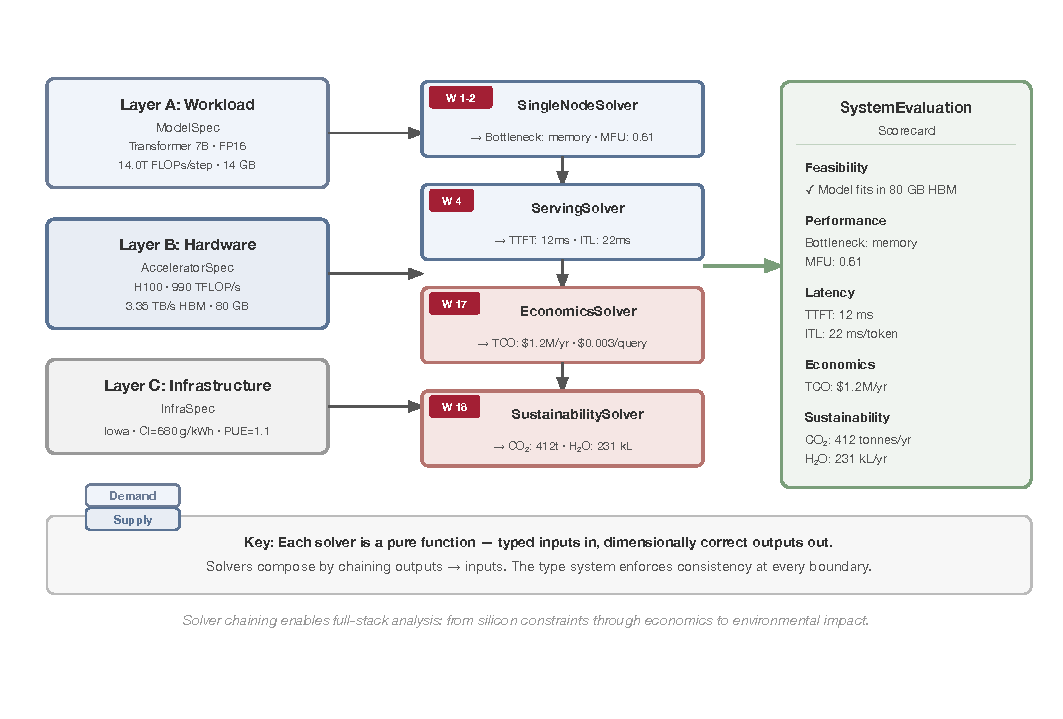
\includegraphics[width=\textwidth]{figures/solver-chaining.pdf}
\caption{\textbf{Resolver Composition.} Three input layers feed four resolvers. Each resolver is a pure function: typed inputs in, dimensionally correct outputs out. The scorecard aggregates three evaluation levels: Feasibility, Performance, and Macro (economics, sustainability, safety).}
\label{fig:solver-chaining}
\end{figure*}

An analytical framework earns trust through transparent confrontation with empirical ground truth. We validate \mlsysim along two axes: \emph{accuracy} against published benchmarks, and the \emph{speed} of design-space exploration. Our goal in validation is not to ``curve-fit'' the model to perfectly match empirical results by introducing arbitrary magic numbers. Rather, it is to demonstrate that a first-principles application of physics and generalized efficiency constants places the prediction squarely in the correct ballpark. As we argue in \Cref{sec:discussion}, a model that is off by 10\% because it structurally ignores L2 cache misses is functioning exactly as intended, trading cycle-level precision for architectural intuition. The anchors below illustrate this philosophy.

The remainder of this section presents the validation in four parts. \Cref{sec:validation-anchors} compares \mlsysim predictions with seven published results spanning single-node training, distributed training, inference, scaling laws, sustainability, and automated parallelism search, and reports each error. \Cref{sec:validation-speed} reports design-space exploration speed. \Cref{sec:accuracy} discusses the accuracy scope and the empirical role of the efficiency parameter $\eta$. Finally, \Cref{sec:validation-dim} argues that runtime dimensional strictness is itself a structural form of validation that numerical accuracy alone cannot supply.

\subsection{Empirical Anchors}
\label{sec:validation-anchors}

We compare \mlsysim predictions with seven published results. Every configuration and number below is computed by the committed generator script (\texttt{paper/scripts/generate\_paper\_values.py}), and \texttt{paper/scripts/validate\_anchors.py} reruns every anchor, reports the error of each comparison with a published measurement, and fails if an identity check or the parallelism search no longer holds. Where an anchor needs the efficiency parameter $\eta$, we state the value used. Those values are chosen per workload class rather than measured, so these anchors test whether one utilization factor places a workload in the right regime and magnitude, not whether the model predicts throughput without calibration.

\textbf{Anchor~1: ResNet-50 on DGX A100 (Single-Node Training).}
For ResNet-50 training on a DGX A100 node (8$\times$ A100 GPUs) at a global batch size of \AnchorOneGlobalBatch{} (\AnchorOnePerGpuBatch{} per GPU), \mlsysim's \texttt{SingleNodeModel} with end-to-end utilization $\eta = \AnchorOneEta$ predicts \AnchorOneSimPerGpu{} samples/s per GPU, or \AnchorOneSimThroughput{} samples/s across the node under ideal intra-node data parallelism, in the \MakeLowercase{\AnchorOneBottleneck}-bound regime. NVIDIA reports \AnchorOneReported{} images/s for this node and per-GPU batch size with mixed precision and XLA~\citep{nvidia2020dleresnet}, so the prediction is \AnchorOneErrorPct\% \AnchorOneErrorDirection{} the measurement. The low $\eta$ reflects that ResNet-50's small convolution kernels, data pipeline, and framework overhead cannot saturate the A100's tensor cores the way large GEMM-dominated Transformer layers can.

\textbf{Anchor~2: Llama-2-70B Decode on H100 (Inference Floor).}
For autoregressive decoding of Llama-2-70B (FP16, batch size 1), the weights total \AnchorTwoWeightsGB\,GB, requiring at least \AnchorTwoTpDegree{} tensor-parallel H100s. \mlsysim's first-order estimate divides total weights by aggregate bandwidth, $\AnchorTwoWeightsGB\;\text{GB} / (\AnchorTwoTpDegree \times \RegHhBandwidthTBs\;\text{TB/s}) = \AnchorTwoDecodeFloorMs$\,ms per token. This is a memory-bandwidth floor that excludes KV-cache reads, NVLink synchronization, and scheduler overhead. We report it without an error because we have not found a published measurement for this exact configuration; it stays in the table as the inference-side regime check.

\textbf{Anchor~3: Llama~3 Training at 16K H100s (Distributed Training).}
Meta's Llama~3 report~\citep{llama3team2024} documents \AnchorThreeReportedMfuPct\% BF16 MFU for 405B pre-training on \AnchorThreeGpus{} H100 GPUs with TP=8, PP=16, and DP=128 at an 8{,}192-token sequence length, on a 400\,Gb/s RoCE fabric, with fully sharded data parallelism for optimizer states and gradients and without activation checkpointing. We configure \mlsysim's \texttt{DistributedModel} with that layout (TP=\AnchorThreeTp, PP=\AnchorThreePp, DP=\AnchorThreeDp, ZeRO stage~\AnchorThreeZeroStage), \AnchorThreeBatch{} sequences of \AnchorThreeSeqLen{} tokens per step, which leaves one sequence for each of at most \AnchorThreeMicrobatches{} pipeline microbatches per DP group, the registry's \AnchorThreeFabricGbps\,Gb/s InfiniBand NDR fabric in place of RoCE, compute--communication overlap $\eta_{\text{overlap}} = \AnchorThreeOverlap$, and $\eta = \AnchorThreeEta$. It predicts an aggregate MFU of \AnchorThreeMfuPct\%, \AnchorThreeErrorPct\% below the reported value (\AnchorThreeErrorPoints{} percentage points). The miss is structural. With \AnchorThreeMicrobatches{} microbatches the 1F1B bubble adds \AnchorThreeBubbleSeconds\,s of idle time to \AnchorThreeComputeSeconds\,s of compute, \AnchorThreeBubbleShareOfStepPct\% of the modeled step. Meta instead runs an interleaved schedule that divides the bubble by the number of virtual stages per pipeline rank, which the report does not give, and frees stage tensors as soon as they are no longer needed. Without those two optimizations \mlsysim's activation accounting also places this layout at \AnchorThreeMemoryGB\,GB per GPU, above the \AnchorThreeCapacityGB\,GB of an H100, although Meta trains it without checkpointing. The anchor therefore marks the limit of a plain 1F1B pipeline model rather than testing $\eta$.

\textbf{Anchor~4: PaLM Model FLOPs Utilization (Pod-Scale Training).}
Google's PaLM-540B~\citep{chowdhery2022palm} was trained without pipeline parallelism on \AnchorFourChips{} TPU~v4 chips in two pods of \AnchorFourPodChips{} chips. Within each pod it used 12-way model parallelism and 256-way fully sharded data parallelism, across the two pods it used data parallelism over the datacenter network, and it rematerialized activations, achieving \AnchorFourReportedMfuPct\% MFU and \AnchorFourReportedHfuPct\% hardware FLOPs utilization; the difference is the rematerialization FLOPs that hardware utilization counts and MFU excludes. We model each pod as one ICI domain at the TPU~v4's \AnchorFourIciGBs\,GB/s per direction~\citep{jouppi2023tpu} and the cross-pod link at \AnchorFourDcnPerChipGBs\,GB/s per chip, which spreads PaLM's reported aggregate burst of \AnchorFourDcnBurstTbps\,Tbps over all chips and is therefore a floor on capacity. With TP=\AnchorFourTp, DP=\AnchorFourDp, ZeRO stage~\AnchorFourZeroStage, full recomputation, a global batch of \AnchorFourBatch{} sequences of \AnchorFourSeqLen{} tokens, TPU~v4 compute of \AnchorFourTflops\,TFLOP/s, and $\eta = \AnchorFourEta$, each chip holds \AnchorFourMemoryGB\,GB of training state, the scaling efficiency is \AnchorFourScalingEffPct\%, and the predicted aggregate MFU is \AnchorFourMfuPct\%, \AnchorFourErrorPct\% below the reported value. Communication costs little in this layout, so the gap sits mostly in $\eta$. Recomputation leaves each replica's model FLOPs utilization at \AnchorFourReplicaMfuPct\%, while PaLM's \AnchorFourReportedHfuPct\% hardware utilization implies a kernel efficiency well above the $\eta = \AnchorFourEta$ we assume.

\textbf{Anchor~5: Chinchilla Scaling Law (Implementation Consistency).}
The Chinchilla paper~\citep{hoffmann2022chinchilla} establishes that compute-optimal training uses about \WallElevenTokensPerParam{} tokens per parameter. \mlsysim's \texttt{ScalingModel} uses the compute approximation $C = 6PD$ and derives the optimal allocation $P^{*} = \sqrt{C/120}$. For Chinchilla's own budget, $C = 6 \times 70\text{B} \times 1.4\text{T} \approx \AnchorFiveComputeBudget$ FLOPs, the solver returns $P^{*} = \AnchorFiveOptimalParamsB$B and $D^{*} = \AnchorFiveOptimalTokensT$T. This is an implementation consistency check rather than an independent validation, because Chinchilla's 1.4T tokens are exactly 20 times its 70B parameters, so $P^{*}$ returns 70B by construction.

\textbf{Anchor~6: Training Carbon Footprint (Unit Consistency).}
\citet{patterson2021carbon} estimate that training GPT-3 on V100 GPUs consumed \AnchorSixEnergyMWh\,MWh and emitted \AnchorSixReportedTonnes{} tonnes CO$_2$e using the 2020 US average grid intensity (\AnchorSixGridCi~gCO$_2$e/kWh). \mlsysim's \texttt{carbon\_from\_energy} reproduces \AnchorSixCarbonTonnes{} tonnes from those inputs. Since the published figure is itself this product, the anchor checks unit handling, not emissions accuracy.

\textbf{Anchor~7: Llama~3 Parallelism Strategy (Optimizer Search).}
To exercise the Tier 3 design-space search, we configure the \texttt{ParallelismOptimizer} with the Llama~3 405B model, its \AnchorThreeGpus-GPU H100 cluster~\citep{llama3team2024}, and Meta's 8{,}192-token sequences. The optimizer sweeps power-of-two TP and PP degrees, pre-screens each candidate so that the per-GPU shard of weights, gradients, and Adam optimizer state fits in 90\% of HBM, prices each survivor with the \texttt{DistributedModel}, drops any whose training state no longer fits once activations are counted, and ranks the \AnchorSevenCandidates{} remaining candidates by MFU. Because \mlsysim's activation accounting admits no split at this sequence length without recomputation (Anchor~3), the search runs with full activation recomputation. It selects TP=\AnchorSevenTp, PP=\AnchorSevenPp, DP=\AnchorSevenDp, the TP=8, CP=1, PP=16, DP=128 layout Meta reports for this stage; Meta uses context parallelism only in its 131K-token stage. The match is narrow, since the winning split beats the runner-up (TP=\AnchorSevenRunnerUpTp, PP=\AnchorSevenRunnerUpPp) by only \AnchorSevenRunnerUpMarginPct\% in MFU. It does not depend on the optimizer's default cap of TP at the node size, because raising the cap to \AnchorSevenWideMaxTp{} returns the same TP=\AnchorSevenWideTp, PP=\AnchorSevenWidePp{} split.

\begin{table*}[t]
\centering
\caption{\textbf{Validation Summary.} Predicted versus reported values for the seven anchors. Error is $|(\text{pred.} - \text{rep.}) / \text{rep.}|$. Anchors~5 and~6 reproduce the arithmetic that defines the published value and are consistency checks. Every predicted value is regenerated from the released package.}
\label{tab:validation}
\small
\renewcommand{\arraystretch}{1.15}
\begin{tabularx}{\textwidth}{@{}X X X r@{}}
\toprule
\textbf{Anchor} & \textbf{Predicted} & \textbf{Reported} & \textbf{Error} \\
\midrule
1: ResNet-50 DGX A100 & \AnchorOneSimThroughput{} samples/s & \AnchorOneReported{} images/s & \AnchorOneErrorPct\% \\
2: Llama-2 70B decode floor (TP=\AnchorTwoTpDegree) & \AnchorTwoDecodeFloorMs\,ms/token & not measured & -- \\
3: Llama~3 405B MFU & \AnchorThreeMfuPct\% & \AnchorThreeReportedMfuPct\% & \AnchorThreeErrorPct\% \\
4: PaLM-540B MFU & \AnchorFourMfuPct\% & \AnchorFourReportedMfuPct\% & \AnchorFourErrorPct\% \\
5: Chinchilla $P^*$ & \AnchorFiveOptimalParamsB B & 70B & identity \\
6: GPT-3 CO$_2$e & \AnchorSixCarbonTonnes\,t & \AnchorSixReportedTonnes\,t & identity \\
7: Llama~3 parallelism & TP=\AnchorSevenTp, PP=\AnchorSevenPp, DP=\AnchorSevenDp & TP=8, PP=16, DP=128 & exact match \\
\bottomrule
\end{tabularx}
\end{table*}

The seven anchors exercise the Node, Algorithm, Fleet, and Operations domains and both Roofline regimes; the Data and Analysis domains have no published anchor yet. \Cref{tab:validation} summarizes the results.

Registry entries record \texttt{metadata.provenance} (\Cref{sec:speed}). Datasheet, literature, and industry-report numbers require a verified URL and date, estimates and derived values require documented justification, and the provenance audit tool (\texttt{mlsysim.tools.audit\_provenance}) fails on any value in the core registries whose provenance is missing or weak, which keeps ``magic numbers'' from accumulating silently as the framework evolves.

\subsection{Design-Space Exploration Speed}
\label{sec:validation-speed}

On an \MachineCpu{} laptop (Python~\MachinePython), \mlsysim's \texttt{SingleNodeModel} evaluates \SweepTimingConfigs{} hardware--model--batch configurations in \SweepTimingMedianMs\,ms (median of five warm runs), about \SweepTimingPerConfigUs\,$\mu$s per configuration. For comparison, ASTRA-sim~2.0 reports 21.42 minutes to simulate a single 1\,MB AllReduce on 64 NPUs with its cycle-level network backend and 1.70 seconds with its analytical backend~\citep{won2023}. These measurements are not like-for-like, since ASTRA-sim models collective communication at much higher fidelity, but they place \mlsysim's per-configuration cost several orders of magnitude below cycle-level simulation. Sub-second execution enables interactive parametric sweeps (e.g., varying HBM bandwidth, substituting fat-tree for torus topology, or relocating the datacenter from Iowa to Qu\'ebec) that would be impractical with cycle-level simulation.

\subsection{Accuracy Scope and Limitations}
\label{sec:accuracy}

\mlsysim provides first-order estimates, not cycle-accurate predictions. We do not re-derive the resolver abstraction here. It is the same first-principles structural bounds plus a single efficiency~$\eta$ for unmodeled second-order effects, as in \Cref{sec:intro,sec:philosophy}. \textbf{Calibrating $\eta$ for validation.} $\eta$ is the one free parameter in the throughput and MFU anchors, and we select it per workload class ($\eta = \AnchorOneEta$ for ResNet-50 training on A100, \AnchorThreeEta{} for Llama~3 405B, and \AnchorFourEta{} for PaLM). These values are chosen per workload class, neither fitted to the reported results nor measured, so those anchors test whether one utilization factor combined with first-principles memory and communication models lands in the correct regime and magnitude. The Roofline parallel (peak versus achievable ceilings, and which constraint binds) is stated in \Cref{sec:intro}; see \citet{williams2009}. Anchors~5 and~6 need no efficiency parameter, but both reproduce the arithmetic that defines the published value, so they check implementation consistency rather than physical accuracy. \Cref{sec:discussion} details the specific phenomena this abstraction cannot capture and the resulting accuracy boundaries.

For \mlsysim's intended use cases (architectural reasoning, lab exercises, capacity planning, and design-space exploration), first-order accuracy is sufficient and often preferable. A student who understands \emph{why} a system is memory-bound has learned more than one who can predict its throughput to three decimal places.

To safeguard against drift, a separate set of representative predictions (\texttt{engine.empirical}: ResNet-50 training throughput on A100 and H100, Llama-3-8B decode latency, and GPT-3 training FLOPs) is bound to sourced tolerance bands in the test suite, and \texttt{paper/scripts/validate\_anchors.py} recomputes the anchors in this section, reports the error of each published comparison, and fails when an identity check or the parallelism search no longer holds.

\subsection{Dimensional Correctness as Validation}
\label{sec:validation-dim}

Beyond numerical accuracy, dimensional strictness (\Cref{sec:dimensional}) provides a structural form of validation. Unit mismatches raise immediate errors rather than producing silently wrong results, eliminating a category of bugs that numerical validation alone cannot catch.

\subsection{Design Invariant Enforcement}
\label{sec:validation-ratchets}

Dimensional strictness (\Cref{sec:dimensional}) catches unit errors at runtime. A complementary question is whether the framework's \emph{architectural} invariants hold as the codebase evolves: do all hardware specifications flow through typed registries? Does every formula carry \texttt{pint} units end-to-end? Can a contributor accidentally reintroduce a bare constant that bypasses the registry? \mlsysim answers these with five machine-checked structural invariants, enforced by a test suite of \CountTests{} tests, each encoding a design decision that would otherwise erode through incremental changes:

\begin{enumerate}[leftmargin=*,itemsep=2pt]
\item \textbf{Specification separation.} There is no constants module at all: the legacy \texttt{core/constants.py} was deleted outright once its last value migrated, and a CI gate now pins its \emph{absence} (any attempt to reintroduce the module, or a compatibility shim for it, fails). Every domain figure lives in its category registry; measurement units live in \texttt{core.units}.
\item \textbf{Loader contract.} The YAML registry loader rejects duplicate keys outright and requires every \texttt{@tech:} and \texttt{@prov:} reference to resolve, so a typo in a data file fails at import rather than silently shadowing or orphaning a specification.
\item \textbf{Provenance coverage.} A dedicated audit (\texttt{mlsysim.tools.audit\_provenance}, also run as a test) walks every registry leaf and fails on missing or weak provenance, enforcing the kind-specific evidence rules of \Cref{sec:speed} across the core registries.
\item \textbf{Cross-registry consistency.} When the same physical quantity appears in multiple registries (e.g., NVLink bandwidth in both \textbf{Hardware} and \textbf{Systems} node definitions), a dedicated check verifies that the DGX node definitions agree with their accelerator entries. This prevents silent divergence between overlapping specification surfaces.
\item \textbf{Registry immutability.} Every registry entry is a frozen \texttt{pydantic} model: attribute assignment raises at the call site. Entries are shared singletons read by every notebook cell in a rendering process, so without this guarantee a single stray write (\texttt{H100.tdp = ...}) would silently corrupt every downstream calculation; with it, the mistake fails loudly where it happens. Code that needs a perturbed variant builds an explicit copy (\texttt{model\_copy}).
\end{enumerate}

Provenance and loader checks apply to every new registry entry automatically, while the cross-registry check covers the DGX node definitions. Empirical-anchor tests (\texttt{engine.empirical}) complete the picture by binding representative solver outputs to sourced benchmark envelopes. The effect is that the zoo architecture described in \Cref{sec:stack} is not merely documented but \emph{enforced}, so the framework's design decisions survive community contributions and long-term evolution.

\section{Usage \& Case Studies}
\label{sec:usage}

\mlsysim is designed for three audiences: students developing quantitative reasoning skills, instructors preparing demonstrations, and researchers evaluating design trade-offs. We present two representative use cases per persona, each illustrating how solvers compose to answer questions that span multiple walls. For a cookbook of runnable code examples demonstrating how users define hardware, perform algebraic design-space sweeps, and invoke SLA-driven hardware synthesis programmatically in Python, see the Appendix (Listings~\ref{lst:speculative},~\ref{lst:appendix-sweep},~\ref{lst:appendix-compose},~\ref{lst:appendix-data},~\ref{lst:appendix-synthesis},~\ref{lst:appendix-speculative},~\ref{lst:appendix-scorecard},~\ref{lst:appendix-optimizer}, and~\ref{lst:appendix-edge}).

\subsection{Student Use Cases}

Students interact with \mlsysim primarily through single-solver queries, short resolver chains, and browser-friendly exercises in the companion textbook. Students can manipulate hardware parameters (e.g., batch size, SLA targets, carbon taxes) and observe how binding constraints shift without needing a backend server or physical hardware.

We present two examples chosen to illustrate complementary aspects of the framework. The first (S1) demonstrates \emph{vertical} resolver composition, chaining inference and economics models to connect an algorithmic decision (chain-of-thought reasoning) to its infrastructure cost. The second (S2) demonstrates \emph{horizontal} composition, combining data-pipeline and compute models to diagnose a bottleneck that moves from the accelerators to the CPU input pipeline.

\subsubsection{S1: Chain-of-Thought Cost}
A student investigates the inference economics of chain-of-thought (CoT) prompting. Using Llama-3 70B on H100 hardware, they configure the \texttt{InferenceScalingModel} with $K{=}8$ reasoning steps. Each step generates $\sim$50 tokens (the calibrated default) at the memory-bound decode rate, so the total reasoning time is $T_{\text{reason}} = \text{TTFT} + K \cdot 50 \cdot \text{ITL}$. The solver reports a total reasoning time of ${\sim}17.9$\,s, a $6.5{\times}$ per-query \emph{latency} multiplier relative to a single-step answer (the one-time prefill TTFT amortizes across the $K$ steps). The \emph{cost} multiplier is larger and tracks total work rather than latency: CoT generates $8{\times}$ as many decode tokens ($K \cdot 50$ vs.\ 50), and because decode is memory-bandwidth-bound the serving throughput is set by token volume. Feeding this into the \texttt{EconomicsModel}, a deployment sized for 100~QPS of single-pass queries must grow its H100 fleet, and hence its TCO, by ${\sim}8{\times}$ to sustain the same query rate under CoT. The two multipliers are distinct: \mlsysim shows chain-of-thought taxes both latency and infrastructure cost, but by different factors.

\subsubsection{S2: CPU Pipeline Bottleneck}
A student configures ResNet-50 training on a DGX A100 (8 GPUs) with a batch size of \CaseSTwoBatch. At a kernel-level efficiency of $\eta = \CaseSTwoEta$, the \texttt{DistributedModel} evaluated on a single DGX A100 node predicts a step time of ${\sim}\CaseSTwoStepMs$\,ms, a demand rate of ${\sim}\CaseSTwoDemandImgPerS$ images/s. Adding the \texttt{DataModel} rules out storage I/O. With \CaseSTwoWorkers{} CPU workers (\CaseSTwoWorkersPerGpu{} per GPU) decoding ImageNet JPEGs at \CaseSTwoDecodeRate{} images/s each, the raw decode pipeline delivers \CaseSTwoRawSupplyImgPerS{} images/s. This appears sufficient, but the \texttt{TransformationModel} accounts for the full augmentation pipeline (random crop, color jitter, normalization) at \CaseSTwoAugmentRate{} images/s per worker, reducing effective throughput to \CaseSTwoEffectiveSupplyImgPerS{} images/s, below the GPUs' \CaseSTwoDemandImgPerS{} images/s appetite. The student discovers that the binding constraint shifts from the accelerators to Wall~9 (Transformation). The GPUs have spare cycles, accelerator utilization falls to \CaseSTwoAccelUtilizationPct\%, and the achieved end-to-end efficiency drops to $\eta \approx \CaseSTwoEndToEndEta$, the same kind of gap between kernel-level and end-to-end efficiency that Anchor~1 absorbs into $\eta = \AnchorOneEta$ (\Cref{sec:validation-anchors}).

\subsection{Instructor Use Cases}

Instructors need demonstrations that run in real time, produce concrete numbers, and connect cleanly to lecture narratives. The following cases show how \mlsysim turns abstract concepts into live, interactive classroom demonstrations.

\subsubsection{I1: Live Roofline Demo, Batch Size Sweep}
An instructor demonstrates the Roofline model by sweeping batch size from 1 to 256 on an H100 for ResNet-50 inference at $\eta = \CaseIOneEta$. At each batch size, the \texttt{SingleNodeModel} returns the bottleneck label, the arithmetic intensity, and the MFU:

\begin{center}
\small
\begin{tabularx}{\columnwidth}{@{}rXlr@{}}
\toprule
Batch & Bottleneck & AI (FLOP/B) & MFU \\
\midrule
1   & \CaseIOneBottleneckBatchOne   & \CaseIOneAiBatchOne   & \CaseIOneMfuBatchOne \\
8   & \CaseIOneBottleneckBatchEight  & \CaseIOneAiBatchEight  & \CaseIOneMfuBatchEight \\
32  & \CaseIOneBottleneckBatchThirtyTwo  & \CaseIOneAiBatchThirtyTwo  & \CaseIOneMfuBatchThirtyTwo \\
128 & \CaseIOneBottleneckBatchOneTwentyEight  & \CaseIOneAiBatchOneTwentyEight  & \CaseIOneMfuBatchOneTwentyEight \\
256 & \CaseIOneBottleneckBatchTwoFiftySix  & \CaseIOneAiBatchTwoFiftySix  & \CaseIOneMfuBatchTwoFiftySix \\
\bottomrule
\end{tabularx}
\end{center}

The crossover from memory-bound to compute-bound occurs between batch \CaseIOneCrossoverLowBatch{} and batch \CaseIOneCrossoverHighBatch, where the arithmetic intensity crosses the effective ridge point $\eta \times F_{\text{peak}} / \text{BW}_{\text{HBM}} \approx \CaseIOneEffectiveRidge$\,FLOP/byte; batching amortizes the one-time weight read across samples, while per-sample activation traffic bounds the gain. MFU keeps climbing past the crossover (\CaseIOneMfuBatchEight{} $\to$ \CaseIOneMfuBatchTwoFiftySix) as the fixed dispatch and per-layer framework taxes amortize. \Cref{fig:roofline} visualizes this transition on the Roofline diagram. The contrast case makes the deeper point. Repeating the sweep for a 7B-parameter LLM \emph{decode} workload shows the arithmetic intensity saturating near \CaseIOneContrastAiMax\,FLOP/byte, far left of the ridge, because KV-cache and activation reads grow with the batch; decode remains memory-bound at every batch size (Walls~4--5). The five-point sweep executes in about \CaseIOneSweepMs\,ms, enabling real-time interaction during lecture.

\begin{figure}[!t]
\centering
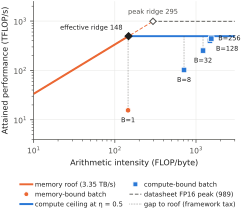
\includegraphics[width=\columnwidth]{figures/roofline-crossover.pdf}
\caption{\textbf{Roofline Crossover: ResNet-50 Batch Size Sweep on H100.} Increasing batch size moves the operating point rightward along the Roofline, transitioning from memory-bound (purple) to compute-bound (cyan) between batch \CaseIOneCrossoverLowBatch{} and batch \CaseIOneCrossoverHighBatch. The peak ridge point is $\RegHhPeakTflops/\RegHhBandwidthTBs \approx \RegHhRidgePoint$\,FLOP/byte; at $\eta = \CaseIOneEta$ the effective ridge sits at ${\approx}\CaseIOneEffectiveRidge$\,FLOP/byte. MFU continues rising past the crossover as dispatch and framework overheads amortize.}
\label{fig:roofline}
\end{figure}

\subsubsection{I2: Iowa vs.\ Qu\'ebec Carbon}
An instructor poses a policy question: \emph{does geography matter for carbon footprint?} They configure a \CarbonFigGpus-GPU cluster (\texttt{Systems.Clusters.Research\_256}) running a training job for \CarbonFigDays{} days at MFU \CarbonFigMfu, and the \texttt{SustainabilityModel} computes emissions under two registered datacenter profiles: an illustrative high-carbon reference profile labeled Iowa (\RegGridIowaCarbonIntensity~gCO$_2$/kWh, PUE \RegGridIowaPue) and Qu\'ebec (hydroelectric, \RegGridQuebecCarbonIntensity~gCO$_2$/kWh, PUE \RegGridQuebecPue). The configuration is identical in hardware and MFU, yet the run emits \CarbonFigIowaTonnes{} tonnes CO$_2$ under the Iowa profile versus \CarbonFigQuebecTonnes{} tonnes in Qu\'ebec, a $\CarbonFigRatio{\times}$ gap, demonstrating that grid carbon intensity is a first-order systems design variable (Wall~18). \Cref{fig:carbon} visualizes this contrast.
\afterpage{%
\begin{figure}[!t]
\centering
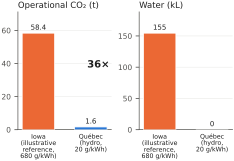
\includegraphics[width=\columnwidth]{figures/carbon-comparison.pdf}
\caption{\textbf{Geography as a Systems Variable: Iowa vs.\ Qu\'ebec.} An identical \CarbonFigGpus-GPU cluster running for \CarbonFigDays{} days at MFU \CarbonFigMfu{} emits $\CarbonFigRatio{\times}$ more CO$_2$ under the illustrative Iowa reference profile (\RegGridIowaCarbonIntensity~gCO$_2$/kWh, PUE \RegGridIowaPue) than in Qu\'ebec (hydroelectric, \RegGridQuebecCarbonIntensity~gCO$_2$/kWh, PUE \RegGridQuebecPue), \CarbonFigIowaTonnes{} vs.\ \CarbonFigQuebecTonnes{} tonnes. Hardware and MFU are identical; only the regional grid profile differs between the two sites.}
\label{fig:carbon}
\end{figure}%
}

\subsection{Researcher Use Cases}

Researchers need to evaluate architectural alternatives and justify procurement decisions with quantitative evidence. The following cases show how \mlsysim enables rapid what-if analysis across hardware generations and parallelism strategies.

\subsubsection{R1: GPU vs.\ Cerebras Crossover}
A researcher evaluates whether wafer-scale silicon changes the economics of large-model inference, using a user-defined \CaseROneParamsB B-parameter, \CaseROneLayers-layer transformer (the registry has no model of this size). On H100s, the \CaseROneWeightsGB\,GB FP16 checkpoint requires tensor parallelism across \CaseROneGpuTp{} GPUs, and \mlsysim reports a decode-phase ITL of $\CaseROneWeightsGB\;\text{GB} / (\CaseROneGpuTp \times \RegHhBandwidthTBs\;\text{TB/s}) \approx \CaseROneGpuItlMs$\,ms/token at batch 1 (memory-bound). The \texttt{WeightStreamingModel} then models the Cerebras WSE-3 with a MemoryX injection bandwidth of \CaseROneInjectionTBs\,TB/s (Cerebras has not published an official MemoryX bandwidth figure, so this value is an estimate). At batch size 1 the weights must stream from MemoryX at this rate, yielding ${\sim}\CaseROneLatencyBatchOneMs$\,ms per token, far \emph{slower} than the GPU cluster. \Cref{eq:weightstream} places the optimal batch at $B^{*} \approx \CaseROneOptimalBatch$ for $\eta = \CaseROneEta$, where injection cost would fully amortize, but at that batch the per-request KV-cache and activation state exceed the \CaseROneWaferSramGiB\,GiB wafer SRAM by roughly $\CaseROneWaferUtilizationAtOptimal{\times}$ and the solver marks the configuration \CaseROneFeasibleAtOptimal. The largest feasible batch is \CaseROneMaxFeasibleBatch, where the wafer delivers ${\sim}\CaseROneThroughputMaxFeasible$ tokens/s. The binding constraint therefore shifts from $\text{BW}_{\text{inject}}$ at small batches to on-wafer memory at large ones, illustrating that the optimal architecture depends on batch size and on where request state can live.

\subsubsection{R2: Hardware Procurement Audit}
A researcher preparing a hardware procurement recommendation for LLM inference needs to answer: \emph{should the next-generation cluster prioritize FLOPS or bandwidth?} The \texttt{SensitivitySolver} perturbs each hardware parameter by 10\% and reports the normalized latency response, shown here for a single-GPU-resident Llama-3 8B decode workload:

\begin{lstlisting}[caption={\textbf{Sensitivity Analysis.} Identifying the binding constraint via 10\% hardware perturbations.},label={lst:sensitivity}]
import mlsysim
from mlsysim.solvers import SensitivitySolver
solver = SensitivitySolver()
res = solver.solve(model=mlsysim.Models.Language.Llama3_8B,
                   hardware=mlsysim.Hardware.Cloud.A100)
print(res.sensitivities)
# {'peak_flops': (*@\WallTwentyOneFlopsSensitivity@*), 'memory_bandwidth': (*@\WallTwentyOneBandwidthSensitivity@*),
#  'memory_capacity': 0.0}
print(f"Binding: {res.binding_constraint}")
# Output: Binding: (*@\WallTwentyOneBinding@*)
\end{lstlisting}

The result is unambiguous. A \WallTwentyOnePerturbationPct\% increase in HBM bandwidth cuts decode latency by \WallTwentyOneBandwidthCutPct\%, whereas a \WallTwentyOnePerturbationPct\% increase in peak FLOPS yields nothing at all, because batch-1 decode sits strictly on the memory roof of \Cref{eq:bottleneck}. The \texttt{SynthesisSolver} then performs the inverse solve. Given a \WallTwentyTwoTargetMs\,ms inter-token latency SLA for Llama-3 70B, it derives the minimum required bandwidth as $\text{BW}_{\text{req}} = |W| / T_{\text{target}} \approx \WallTwentyTwoRequiredBwGBs$\,GB/s, $\WallTwentyTwoAhMultiple{\times}$ the A100's \RegAhBandwidthTBs\,TB/s, confirming that Llama-3 70B inference is firmly in the memory-bound regime and that hardware procurement should prioritize HBM bandwidth over peak throughput.

\subsubsection{R3: End-to-End Llama-3 70B Training Audit}
To illustrate how \mlsysim's solvers compose across the taxonomy, we trace a training analysis for Llama-3 70B on the registered \texttt{Training\_512\_H100} fleet (\CaseRThreeNodes{} DGX H100 nodes and \CaseRThreeGpus{} GPUs, NVLink intra-node and \CaseRThreeFabricGbps\,Gb/s \CaseRThreeFabric{} inter-node) with a global batch of \CaseRThreeBatch{} sequences of \CaseRThreeSeqLen{} tokens, TP=\CaseRThreeTp{} within each node, DP=\CaseRThreeDp, and $\eta = \CaseRThreeEta$.

\textbf{Node (Walls 1--2).} Without optimizer sharding or recomputation, the TP=\CaseRThreeTp{} training state exceeds an 80\,GB H100, so the audit adds ZeRO-1 optimizer sharding across the DP group and full activation recomputation. The \texttt{DistributedModel} then evaluates one tensor-parallel replica with the Roofline core and predicts \CaseRThreeComputeSeconds\,s of compute per step, and the \texttt{TrainingMemoryModel} reports \CaseRThreePerGpuMemoryGB\,GB of training state per GPU, which \CaseRThreeMemoryFits{} the HBM. Recomputation costs a fourth forward pass, so the replica's model FLOPs utilization is \CaseRThreeReplicaMfuPct\% at $\eta = \CaseRThreeEta$.

\textbf{Algorithm (Wall 11).} A 30-day run at the predicted step time processes ${\sim}\CaseRThreeTokensT$T tokens, a budget of $C \approx \CaseRThreeFlopBudget$ FLOPs, for which the \texttt{ScalingModel} gives a Chinchilla-optimal model size of $P^{*} \approx \CaseRThreeChinchillaPstarB$B.

\textbf{Fleet (Walls 14--15).} Communication adds \CaseRThreeTpCommMs\,ms of tensor-parallel AllReduce and \CaseRThreeDpCommMs\,ms of data-parallel gradient synchronization per step, of which \CaseRThreeDpExposedMs\,ms is exposed after compute--communication overlap, for a step time of \CaseRThreeStepSeconds\,s, a scaling efficiency of \CaseRThreeScalingEffPct\%, and a fleet MFU of \CaseRThreeMfuPct\%. The \texttt{ReliabilityModel} estimates a fleet MTBF of \CaseRThreeFleetMtbfHours\,hours, a Young--Daly checkpoint interval of ${\sim}\CaseRThreeCheckpointIntervalMin$\,minutes, about \CaseRThreeExpectedFailures{} failures over 30 days, and a goodput of \CaseRThreeGoodputPct\%.

\textbf{Operations (Walls 17--18).} In Qu\'ebec, the \texttt{EconomicsModel} projects \$\CaseRThreeCapexK{}K of amortized CapEx, \$\CaseRThreeEnergyK{}K of energy, and \$\CaseRThreeMaintenanceK{}K of maintenance, a run TCO of ${\sim}$\$\CaseRThreeTcoM{}M. The \texttt{SustainabilityModel} estimates \CaseRThreeEnergyMWh\,MWh of facility energy and \CaseRThreeCarbonTonnes{} tonnes CO$_2$, $\CaseRThreeIowaRatio{\times}$ less than the \CaseRThreeIowaCarbonTonnes{} tonnes under the Iowa reference profile.

\textbf{Analysis (Walls 21--22).} The \texttt{SensitivitySolver} and \texttt{SynthesisSolver} operate on a single device, so a fleet-level what-if instead re-runs the chain with a changed fabric, node count, or region, which takes ${\sim}\CaseRThreeChainSeconds$\,s per evaluation.

This trace exercises Walls~1, 2, 11, 14, 15, 17, and 18 through a single model, demonstrating how solver composition produces a system assessment from individual physics-based constraint equations.

\subsubsection{R4: Automated Parallelism Search}
A researcher needs to schedule a 175B-parameter model on a new 2{,}048-GPU cluster. Manually searching the 3D-parallelism space ($\text{TP} \times \text{PP} \times \text{DP}$) is error-prone. A split that maximizes DP might exceed the 80\,GB HBM capacity, while a split that maximizes TP might saturate the NVLink interconnect. Instead of trial and error, the researcher invokes a Tier 3 Optimizer. They configure the \texttt{ParallelismOptimizer} with the workload, the cluster, a global batch of \CaseRFourBatch{} sequences, and $\eta = \CaseRFourEta$. It maximizes MFU over power-of-two factorizations with TP capped at the node size. A quick screen drops splits whose per-GPU weights, gradients, and Adam optimizer state exceed 90\% of HBM ($\CaseRFourScreenCapGB$\,GB); the \texttt{DistributedModel} then prices each survivor with one-sequence pipeline microbatches and drops any whose training state, activations included, exceeds the \CaseRFourCapacityGB\,GB of an H100, leaving \CaseRFourCandidates{} candidates. In well under a second it returns TP=\CaseRFourTp, PP=\CaseRFourPp, DP=\CaseRFourDp{} (MFU \CaseRFourBestMfuPct\%), with TP matching the intra-node GPU count so tensor-parallel traffic stays off the slower inter-node fabric. PP=\CaseRFourMinPp{} is the shallowest pipeline whose per-GPU training state fits (\CaseRFourStateAtMinPpGB\,GB); halving the pipeline depth would demand \CaseRFourStateBelowMinPpGB\,GB. This demonstrates the power of the ``engineering engine'' to invert the analytical models into automated design-space synthesis.

\section{Fallacies \& Pitfalls}
\label{sec:fallacies}

Following the tradition of \citet{hennessy2024architecture}, we highlight common misconceptions that \mlsysim is designed to expose.

\textbf{Fallacy: Tripling peak FLOP/s triples LLM serving speed.}
A student might assume that upgrading from A100 (\RegAhPeakTflops\,TFLOP/s FP16) to H100 (\RegHhPeakTflops\,TFLOP/s, a $\RegHhOverAhFlopsRatio{\times}$ increase) should yield a $\RegHhOverAhFlopsRatio{\times}$ speedup. \mlsysim's \texttt{SingleNodeModel} reveals why this is false. LLM inference is memory-bandwidth-bound, and the A100-to-H100 bandwidth improvement is only about $\RegHhOverAhBandwidthRatio{\times}$ (\RegAhBandwidthTBs~TB/s $\to$ \RegHhBandwidthTBs~TB/s). For memory-bound decode, token latency scales with bandwidth, not FLOP/s; compute-bound training does see most of the FLOP/s gain. The Roofline model (\Cref{eq:bottleneck}) makes this visible by showing that the binding constraint determines which hardware parameter matters.

\textbf{Fallacy: At 512 GPUs, checkpointing is a bigger tax than communication.}
On the \CaseRThreeFabricGbps\,Gb/s \CaseRThreeFabric{} fleet of Case~R3, the \texttt{DistributedModel} charges \CaseRThreeTpCommMs\,ms of tensor-parallel and \CaseRThreeDpExposedMs\,ms of exposed data-parallel communication to a \CaseRThreeStepSeconds\,s step, a \FallacyCommCommFractionPct\% loss of scaling efficiency. The \texttt{ReliabilityModel}, with a fleet MTBF of \CaseRThreeFleetMtbfHours\,hours and Young--Daly checkpoints every ${\sim}\CaseRThreeCheckpointIntervalMin$\,minutes, charges only \FallacyCommGoodputLossPct\% of goodput to checkpoints and restarts, and that estimate is optimistic because it omits rework. At this scale communication (Wall~14) is the larger tax, and an analysis that blames checkpointing without measuring both would invest in the wrong fix.

\textbf{Pitfall: Using peak bandwidth in back-of-the-envelope calculations.}
Vendor datasheets report peak HBM bandwidth (e.g., \cvalii{\HhBWTBs}\,TB/s for H100), and sustained bandwidth under real access patterns can be lower, so decode estimates built on peak bandwidth are optimistic. \mlsysim applies $\eta$ only to FLOP/s; decode latency uses the registry bandwidth directly, so users who want a sustained-bandwidth estimate should derate \texttt{memory.bandwidth} explicitly (e.g., through \texttt{model\_copy}).

\textbf{Pitfall: Ignoring geography in carbon accounting.}
Two identical training runs produce vastly different environmental impact depending on grid carbon intensity. As demonstrated in Case~I2, the same \CarbonFigGpus-GPU cluster emits $\CarbonFigRatio{\times}$ more CO$_2$ under the Iowa reference profile than in Qu\'ebec. Students who omit Wall~18 (Sustainability) from their analysis miss a first-order systems design variable, one that increasingly affects both cost (carbon pricing) and regulatory compliance.

\textbf{Fallacy: Quantization always provides a linear speedup.}
Reducing precision from FP16 to INT4 ($r_{\text{quant}} = 4{\times}$) reduces memory by $4{\times}$, but the compute speedup depends on whether the workload is memory-bound or compute-bound. For memory-bound LLM decode, most of the $4{\times}$ memory reduction becomes throughput because the bottleneck is weight reads. For compute-bound workloads, the gain depends on low-precision kernel support, so \mlsysim applies the registry's per-precision FLOP/s where an entry exists and falls back to FP16 throughput, with a warning, when it does not. \mlsysim's Roofline analysis makes this regime-dependent behavior explicit.

\section{Discussion \& Limitations}
\label{sec:discussion}

``All models are wrong, but some are useful''~\citep{box1979robustness}. Users must understand the boundaries of \mlsysim's analytical abstraction. We organize the limitations into modeling scope, accuracy trade-offs, and pedagogical implications, then outline future directions.

\subsection{What \mlsysim Cannot Model}

\textbf{No microarchitectural effects.} \mlsysim has no notion of L1/L2 cache hierarchies, branch prediction, kernel scheduling, or register pressure. These second-order effects are absorbed into a single scalar efficiency parameter ($\eta$, the ratio of sustained to peak FLOP/s). While $\eta$ provides a serviceable approximation for back-of-the-envelope reasoning, it cannot capture workload-dependent microarchitectural behavior; a matrix multiply and a sparse attention kernel may achieve very different $\eta$ on identical silicon.

\textbf{No real network congestion.} The communication model uses the classical $\alpha$-$B_{\text{link}}$ formulation (latency plus inverse-bandwidth), which assumes dedicated links. \mlsysim does not model adaptive routing, network contention under multi-tenant traffic, or congestion collapse, phenomena that become critical at scales beyond $\sim$10{,}000 nodes, precisely the regime where ASTRA-sim~2.0~\citep{won2023} provides essential fidelity. The static bisection view behind Wall~10 (Locality) is optimistic under the same cross-traffic conditions. A scalar \texttt{congestion\_factor} can inflate communication time, but contention dynamics are not modeled.

\textbf{Coarse OS/runtime overhead.} Kernel launch and framework dispatch are folded into a fixed per-device dispatch tax and a per-layer framework tax; CUDA stream scheduling, Python GIL contention, and host--device transfer dynamics are not modeled separately, so small-batch inference predictions are only as good as those two constants.

\textbf{No heterogeneous fleets.} The \texttt{DistributedModel} assumes homogeneous nodes, where all accelerators in a fleet share the same compute, memory, and interconnect specifications. Production clusters increasingly mix hardware generations (e.g., A100 and H100 nodes in the same job), and fleet-level efficiency metrics such as ML Productivity Goodput~\citep{wongpanich2025fleet} capture this heterogeneity. Modeling heterogeneous fleets would require per-node load balancing and straggler analysis beyond the current analytical framework.

\textbf{No dynamic behavior.} \mlsysim models steady-state throughput. Transient effects (thermal throttling, dynamic clock boosting, memory fragmentation over long training runs, and checkpoint I/O contention with concurrent training traffic) are outside its scope. A training run that degrades over 72 hours due to thermal saturation will appear identical to one that sustains peak throughput.

\textbf{Heuristic accuracy models.} The accuracy degradation curves in \texttt{CompressionModel} are heuristic step functions (for quantization) and exponentials (for pruning), not architecture-specific empirical fits. Real accuracy loss depends on model architecture, calibration methodology, and quantization method (e.g., well-calibrated GPTQ INT4 can achieve $<$0.5\% degradation, while naive round-to-nearest may lose 10\%+). Users should treat these curves as directional indicators, not ground truth.

\subsection{Walls Not Included}

The 22-wall taxonomy is comprehensive but not exhaustive. Several constraints were considered and excluded, each for a specific reason.

\textbf{Thermal throttling.} Sustained power density can force throughput below peak TDP, but this is absorbed into $\eta$ rather than modeled as a distinct wall.

\textbf{Resource fragmentation.} Scattered GPU availability across nodes prevents job scheduling even when aggregate capacity is sufficient; this is a combinatorial bin-packing problem beyond the current analytical framework.

\textbf{Compiler/graph optimization.} The gap between a framework's computational graph and the executed kernel schedule affects both latency and MFU, but varies too rapidly across software versions to model analytically.

The selection criterion for inclusion was: does the constraint have a stable, published analytical formulation that remains valid across hardware generations? Constraints requiring empirical trace data or combinatorial optimization were deferred to future work.

\subsection{The Accuracy--Speed Trade-off}

Each omission above reflects the same trade-off: evaluation that is orders of magnitude faster, at the cost of second-order fidelity. The precedent is SPIM, which executes MIPS programs at the instruction-set level and omits pipelining, superscalar execution, and cache hierarchies, prioritizing pedagogical clarity over the full complexity of commercial processors. \mlsysim applies the same philosophy to ML systems, making quantitative reasoning accessible to students who may never operate a production cluster.

The relevant question is not ``How accurate is \mlsysim?'' but ``Does it identify the correct binding constraint?'' A first-order model that correctly determines whether a system is memory-bound, compute-bound, or network-bound provides actionable architectural insight even when its absolute latency prediction is $\pm$20\% from a cycle-accurate trace. The binding constraint dictates which hardware investment yields the largest return, and this ordinal ranking is far more robust than cardinal predictions. Practitioners who know that their system is memory-bandwidth-bound will invest in higher-bandwidth memory regardless of whether the predicted latency is 47\,ms or 53\,ms.

\subsection{Future Work}

We identify several directions for extending \mlsysim.

\textbf{Broader empirical validation.} \Cref{sec:validation} compares seven anchors across four taxonomy domains. Future work will extend this to newer hardware generations already present in the registry (NVIDIA B200/GB200, TPU~v6) as published benchmark results appear, inference serving under load (the continuous-batching model now takes a request-length distribution, but no serving anchor validates it yet), and checkpoint overhead at scale, where published data points are becoming available from reproducibility studies.

\textbf{Community hardware registry.} The \textbf{Hardware} registry currently contains a curated set of hardware entries sourced to manufacturer datasheets where available, with estimates labeled as such in their provenance. We plan to open contributions from the community, with automated verification scripts that cross-check submitted specifications against known physical limits (e.g., memory bandwidth cannot exceed pin count $\times$ data rate).

\textbf{Custom degradation curves.} Future versions will allow users to supply empirically fitted accuracy-compression curves from their own quantization experiments, replacing the current heuristic step and exponential curves with data-grounded models.

\textbf{TinyTorch integration.} \mlsysim provides analytical predictions; TinyTorch~\citep{tinytorch2025}, the companion educational framework, provides implementation-based verification. Connecting the two tools creates a predict-then-verify loop. Students estimate training time and memory consumption in \mlsysim, then run the actual training in TinyTorch and compare. This closed loop reinforces quantitative reasoning by grounding analytical models in empirical observation.

\textbf{Agentic and embodied extensions.} The package already ships two extension registries, \textbf{Agents} (agentic workload profiles) and \textbf{Embodied} (robot platforms), together with the \texttt{agents} and \texttt{robotics} physics modules (\Cref{tab:physics-modules}). They cover trajectory reliability, test-time compute cost, and multi-agent coordination for agents, and sensor-to-actuator latency, safe stopping distance, and action-chunk cadence for robots. We deliberately keep them outside the wall taxonomy. Several of their formulas are modeling assumptions rather than published analytical results, many registry values are labeled estimates, and no resolver or validation anchor exercises them yet. Promoting candidates such as a trajectory-reliability wall or a sensor-to-actuator latency wall would require sourced formulations, dedicated resolvers, and anchors of the kind in \Cref{sec:validation}.

\textbf{Expanding Tier 3 Optimizers (Pareto Frontiers).} Currently, the Tier 3 optimizers search single-dimensional objective spaces (e.g., maximizing MFU or maximizing batch size under a latency constraint); a two-objective compression Pareto sweep already ships in \texttt{CompressionModel.sweep}. Future work will extend the Tier 3 engine to support multi-objective Pareto frontiers, simultaneously optimizing across latency, total cost, carbon footprint, and accuracy. This will enable richer design-space exploration and formally expose the inherent tensions between performance and sustainability.

\subsection{The Pedagogical Argument}

Even when \mlsysim's predictions miss measured values by tens of percent, as Anchors~3 and~4 do (\Cref{sec:validation-anchors}), the pedagogical value lies in the reasoning process rather than the numerical output. A student who sweeps 1{,}000 configurations and identifies memory bandwidth as the binding constraint for LLM inference has acquired a transferable analytical skill, that of determining which resource limits performance. The framework trains students to formulate the correct quantitative questions (arithmetic intensity, ridge point location, communication-to-computation ratio) and these questions generalize to production systems even as specific hardware parameters change across generations.

\section{Conclusion}
\label{sec:conclusion}

Modern ML systems are no longer limited by a single resource that can be optimized in isolation. A deployment decision can hinge simultaneously on arithmetic intensity, memory capacity, communication topology, queueing delay, energy price, regional carbon intensity, and failure recovery. This coupling makes intuition brittle: a faster accelerator may not improve decode latency, a larger batch may move the bottleneck from memory to compute, and a cheaper datacenter may be the wrong choice once emissions or water constraints are included. The practical challenge is to make these interactions visible before teams commit to hardware, cloud spend, or weeks of empirical benchmarking.

\mlsysim treats ML system design as a set of executable constraints. Its purpose is not to replace profilers, trace-driven simulators, or cycle-level models; those tools remain necessary when the question is precise performance on a concrete system. Instead, \mlsysim occupies the earlier stage where engineers and students need to ask which wall binds, which parameter matters, and which design alternatives are worth measuring at all. Its standard is first-order fidelity: close enough to identify bottlenecks and rank alternatives, explicit enough to expose assumptions, and fast enough to explore the design space before measurement begins. By separating demand from supply, carrying units through its hardware, workload, and network calculations, and composing first-principles resolvers across the full stack, it turns informal back-of-the-envelope reasoning into a reproducible infrastructure model.

That artifact is also pedagogical. Paired with TinyTorch~\citep{tinytorch2025} and the open \emph{Machine Learning Systems} text~\citep{mlsysbook2025}, \mlsysim gives learners a way to connect equations, code, and infrastructure consequences without requiring access to a GPU cluster. The goal is not merely to compute a latency or carbon number, but to teach a durable habit of systems reasoning: identify the binding constraint, check the units, perturb the design, and explain why the result changed. As ML systems continue to scale across larger models, heterogeneous fleets, and stricter economic and environmental constraints, that habit will matter as much as any single modeling tool.

\section*{Generative AI Usage Statement}

In developing \mlsysim, the goal was not to formulate new physical laws or mathematical bounds, but to ground ML systems reasoning in first principles---distilling established equations and published constraints from across computer architecture, distributed systems, and machine learning into an executable, dimensionally strict engineering framework. The package was designed specifically as the quantitative substrate for the \emph{Machine Learning Systems} textbook series~\citep{mlsysbook2025}, providing an environment for first-principles architectural reasoning without requiring hardware clusters. Generative AI tools were used throughout this process to assist with cross-disciplinary literature search, locate empirical data points, and draft initial code and test scaffolding from structural blueprints. The author conceived the system architecture, structured the 22-wall taxonomy and progression, designed the software interfaces, and audited every formula, datasheet constant, and solver implementation against its primary source. All calculations are verified by automated dimensional and regression tests, and the author remains solely responsible for the design, implementation, and conclusions presented in this work.

\bibliography{references}


\clearpage
\onecolumn
\begin{appendices}

\section{MLSysBook Integration (LEGO Cells)}
\label{sec:appendix-mlsysbook}

\mlsysim serves as the executable backbone for \emph{Machine Learning Systems}, a four-volume series (\url{https://mlsysbook.ai/vol1}, \url{https://mlsysbook.ai/vol2}, \url{https://mlsysbook.ai/vol3}, and \url{https://mlsysbook.ai/vol4})~\citep{mlsysbook2025}. To integrate quantitative analysis into the prose without disrupting readability, the textbook introduces the concept of \textbf{LEGO Cells}. LEGO is an acronym for the four structural phases of each cell: \textbf{Load} (importing registries and constraints), \textbf{Execute} (invoking the physics solvers), \textbf{Guard} (asserting dimensional and logical invariants), and \textbf{Output} (formatting physical quantities for inline prose). A LEGO Cell is a standalone, self-contained Python snippet that answers a specific design question posed in the text. Isolating the simulation logic into these executable blocks allows readers to read the code to understand the mechanics, execute it to verify the results, and modify the parameters to explore alternative scenarios.

Below, we provide three illustrative cells written in the LEGO style used throughout the textbook. They are simplified for this paper and are not verbatim excerpts; the cells in the books wrap the same four phases in a class with a documented header.

\subsection{Volume 1 Style: Hardware Constraints}
In Volume 1, LEGO Cells are heavily used to explain hardware constraints. For example, when introducing the Roofline model, a LEGO-style cell shows that Llama-3 8B decode on an H100 remains memory-bound even as batch size grows:

\begin{lstlisting}[language=Python, caption={\textbf{Illustrative LEGO-Style Cell: Roofline Analysis.} Sweeping batch size with the \texttt{Engine} shows Llama-3 8B decode remaining memory-bound at every batch size.}, label={lst:lego-vol1}]
from mlsysim.engine.engine import Engine
from mlsysim.hardware.registry import Hardware
from mlsysim.models.registry import Models

model = Models.Language.Llama3_8B
hw = Hardware.Cloud.H100

for b in [1, 16, 128, 512]:
    perf = Engine.solve(model, hw, batch_size=b, precision="fp16")
    print(f"Batch {b}: {perf.bottleneck}-bound, MFU={perf.mfu:.3f}")
\end{lstlisting}

\subsection{Volume 2 Style: Distributed Training}
In Volume 2, the focus shifts to distributed systems and fleet-level economics. LEGO-style cells here compose multiple solvers to estimate the time and cost of training frontier models across thousands of GPUs:

\begin{lstlisting}[language=Python, caption={\textbf{Illustrative LEGO-Style Cell: Training Economics.} Composing solvers to estimate the duration and carbon footprint of a large-scale training run.}, label={lst:lego-vol2}]
from mlsysim.solvers import DistributedModel, SustainabilityModel
from mlsysim.systems.registry import Systems
from mlsysim.models.registry import Models
from mlsysim.infrastructure.registry import Infrastructure

fleet = Systems.Clusters.Frontier_8K
model = Models.Language.Llama3_70B

perf = DistributedModel().solve(
    model, fleet, batch_size=4096, seq_len=4096, tp_size=8, pp_size=8
)
training_days = (perf.step_latency_total * 1e12 / (4096 * 4096)).to("day")

sust = SustainabilityModel().solve(
    fleet, duration_days=training_days.magnitude,
    datacenter=Infrastructure.Datacenters.Iowa_Reference, mfu=0.45
)
print(f"Training Time: {training_days.magnitude:.0f} days")
print(f"Carbon: {sust.carbon_footprint_kg / 1000:.0f} tonnes")
\end{lstlisting}

\subsection{Volume 1 Style: Model Serving}
Another common pattern in Volume 1 evaluates inference systems. Here, a LEGO-style cell uses the \texttt{ServingModel} to calculate the inter-token latency (ITL) for Llama-3 8B on an NVIDIA A100 GPU:

\begin{lstlisting}[language=Python, caption={\textbf{Illustrative LEGO-Style Cell: Model Serving.} The \texttt{ServingModel} estimates the theoretical inter-token latency for an autoregressive generation step. The cell shows the four \textbf{LOAD}, \textbf{EXECUTE}, \textbf{GUARD}, and \textbf{OUTPUT} phases of the LEGO pattern.}, label={lst:lego-vol1-serving}]
from mlsysim.solvers import ServingModel
from mlsysim.models.registry import Models
from mlsysim.hardware.registry import Hardware

# 1. LOAD (Constants)
model = Models.Language.Llama3_8B
hw = Hardware.Cloud.A100

# 2. EXECUTE (The Compute)
perf = ServingModel().solve(
    model, hw, seq_len=1256, batch_size=1, precision="int4", efficiency=1.0
)

# 3. GUARD (Invariants)
assert perf.feasible, "configuration must fit in memory"

# 4. OUTPUT (Formatting)
print(f"Inter-Token Latency (ITL): {perf.itl.to('ms'):.2f}")
\end{lstlisting}

\section{Registry Snapshot}
\label{sec:appendix-hardware}

The MLSys Zoo comprises eight core registries spanning the full systems stack, plus the \textbf{Agents} and \textbf{Embodied} extension registries and the \texttt{Literature} and \texttt{ReferenceStats} auxiliary surfaces. This appendix is a representative snapshot of the current local registry surface: enough to show the kinds of systems \mlsysim can compose, without treating the paper as the authoritative inventory. The typed Python and YAML registry source remains the source of truth for the complete, up-to-date entries.

\subsection{Hardware Registry}

\Cref{tab:hw-catalog} summarizes the current accelerator coverage by deployment tier. Each entry is a fully typed \texttt{HardwareNode} with \texttt{pint}-dimensioned fields. Users add custom entries by instantiating the same types (Listing~\ref{lst:hwnode}), and custom entries participate in the same dimensional pipeline as vetted ones. For example, a research team evaluating a pre-release accelerator can define a speculative entry with projected specifications and immediately sweep it against existing workloads (Listing~\ref{lst:speculative}).

\noindent\begin{minipage}{\textwidth}
\begin{lstlisting}[language=Python, caption={\textbf{Extending the Registry.} Defining a speculative hardware entry using the typed \texttt{HardwareNode} schema (\Cref{tab:type-schema}) for immediate solver evaluation.}, label={lst:speculative}]
from mlsysim.hardware.types import HardwareNode, ComputeCore, MemoryHierarchy
from mlsysim.core.units import TFLOPs, GB, TB, second, watt

custom_accelerator = HardwareNode(
    name="Speculative GPU 2027", release_year=2027,
    compute=ComputeCore(peak_flops=1200 * TFLOPs / second,
                        precision_flops={"fp16": 1200 * TFLOPs / second, "fp8": 2400 * TFLOPs / second}),
    memory=MemoryHierarchy(capacity=144 * GB, bandwidth=5.0 * TB / second),
    tdp=800 * watt,
)
\end{lstlisting}
\end{minipage}

\begin{table}[!t]
\centering
\caption{\textbf{Hardware Registry Snapshot.} All \CountHardwareDevices{} hardware entries in the registry, organized by deployment tier and sorted by peak throughput. Peak FLOP/s is FP16 Tensor Core (or equivalent) throughput; BW is primary-memory bandwidth (HBM, LPDDR, or on-die SRAM as appropriate); memory is binary capacity in GiB.\protect\footnotemark}
\label{tab:hw-catalog}
\footnotesize
\renewcommand{\arraystretch}{1.05}
\begin{tabularx}{\textwidth}{@{}l >{\raggedright\arraybackslash}X r r r r >{\raggedright\arraybackslash}p{3.3cm}@{}}
\toprule
\textbf{Tier} & \textbf{Accelerator} & \textbf{Peak (TFLOP/s)} & \textbf{Mem (GiB)} & \textbf{BW (TB/s)} & \textbf{TDP (W)} & \textbf{Interconnect} \\
\midrule
\HwCatalogRows
\bottomrule
\end{tabularx}
\end{table}
\footnotetext{The Cerebras CS-3 BW is on-wafer SRAM bandwidth. The weight-streaming serving case study (\Cref{sec:usage}) instead uses the \CaseROneInjectionTBs\,TB/s MemoryX injection bandwidth, the off-chip bandwidth the host sees. NVIDIA GB200 NVL72 is a rack-scale system entry (72 Blackwell GPUs behind one NVLink switch domain) rather than a single accelerator.}

\FloatBarrier
\subsection{Infrastructure and Systems Registries}

The Hardware registry (\Cref{tab:hw-catalog}) captures individual accelerator capabilities, but real deployments compose accelerators into nodes, connect nodes through network fabrics, and situate the resulting clusters in datacenters whose geography determines energy cost, carbon intensity, and cooling strategy. The Infrastructure and Systems registries complete this picture: Infrastructure encodes \emph{where} the fleet runs, and Systems encodes \emph{how} accelerators are assembled into distributed configurations. Together the three registries let a single resolver chain evaluate end-to-end metrics from per-device roofline through fleet-level TCO and carbon footprint.

The \textbf{Infrastructure} registry encodes regional environmental context for sustainability analysis, plus datacenter profiles, rack power envelopes, facility cooling, cloud pricing, and capacity lead times. Carbon intensity varies by roughly $\RegGridCarbonSpread{\times}$ across the \CountGridProfiles{} registered grid profiles, making geography a first-order design variable (Case~I2, \Cref{sec:usage}). The \textbf{Systems} registry defines compute nodes, network fabrics, fleet configurations, TPU pods, switch fabrics, and storage and checkpoint-path profiles (NVMe generations, SATA, HDD, object stores, parallel file systems) used by the \texttt{DistributedModel}, \texttt{ReliabilityModel}, and \texttt{DataModel}. \Cref{tab:infra-systems} presents representative entries from both registries.

\begin{table}[!t]
\centering
\caption{\textbf{Infrastructure and Systems Registry Snapshot.} \textit{Top:} Grid profiles for sustainability analysis (CI\,=\,carbon intensity in gCO$_2$/kWh; PUE\,=\,power usage effectiveness; WUE\,=\,water usage effectiveness in L/kWh). \textit{Bottom:} Registered compute nodes, network fabrics, and fleet configurations for distributed analysis.}
\label{tab:infra-systems}
\footnotesize
\renewcommand{\arraystretch}{1.05}
\textbf{Grid Profiles (\CountGridProfiles{} registered)}\\[3pt]
\begin{tabularx}{\textwidth}{@{}>{\raggedright\arraybackslash}X r r r l@{}}
\toprule
\textbf{Profile} & \textbf{CI} & \textbf{PUE} & \textbf{WUE} & \textbf{Source} \\
\midrule
\InfraGridRows
\bottomrule
\end{tabularx}

\vspace{8pt}
\textbf{Nodes, Fabrics, and Fleets}\\[3pt]
\begin{tabularx}{\textwidth}{@{}>{\raggedright\arraybackslash}p{0.42\textwidth} >{\raggedright\arraybackslash}X@{}}
\toprule
\multicolumn{2}{@{}l}{\textit{Compute Nodes (\CountNodes{} registered)}} \\
\midrule
\SystemsNodeRows
\midrule
\multicolumn{2}{@{}l}{\textit{Network Fabrics (\CountFabrics{} registered)}} \\
\midrule
\SystemsFabricRows
\midrule
\multicolumn{2}{@{}l}{\textit{Fleet Configurations (\CountClusters{} registered)}} \\
\midrule
\SystemsClusterRows
\bottomrule
\end{tabularx}
\end{table}

\FloatBarrier
\subsection{Type System and Physics API}

To support the separation of demand and supply, \mlsysim relies on a shallow but rigorously typed hierarchy of Pydantic models (\Cref{tab:type-schema}). These types act as the contract between the declarative registries and the analytical solvers. Because all physical quantities (bandwidth, latency, power) are dimensioned using the \texttt{pint} library, users can extend any registry by instantiating these types directly without risking unit mismatch errors.

Beneath the resolvers lies the Physics Engine, which contains the dimensioned mathematical identities that govern ML systems. \Cref{tab:physics-api} catalogs the public API of these physics modules. Each function is stateless, accepting dimensioned quantities (or raw floats that are immediately coerced to units) and returning dimensioned bounds. These functions implement the core logic for the Iron Law of training, the Roofline model, and network communication topologies.

\begin{table}[!t]
\centering
\small
\renewcommand{\arraystretch}{1.05}
\caption{\textbf{Physics Module Public API.} Selected function signatures organized by domain module. Every function accepts \texttt{pint} \texttt{Quantity} arguments (or raw floats coerced via \texttt{\_ensure\_unit()}) and returns dimensioned quantities. Import from \texttt{mlsysim.physics} (one module per domain).}
\label{tab:physics-api}
\begin{tabularx}{\textwidth}{@{}l l X@{}}
\toprule
\textbf{Module} & \textbf{Function} & \textbf{Signature (key parameters $\to$ return)} \\
\midrule
\multirow{6}{*}{\texttt{performance}} & \texttt{dTime} & (total\_ops, n\_devices, peak\_flops, $\eta$) $\to$ seconds \\
 & \texttt{calc\_bottleneck} & (ops, model\_bytes, device\_flops, device\_bw) $\to$ \{time, regime\} \\
 & \texttt{calc\_amdahls\_speedup} & (parallel\_frac, speedup\_factor) $\to$ overall speedup \\
 & \texttt{calc\_pipeline\_bubble} & (n\_stages, n\_microbatches, v\_stages) $\to$ bubble fraction \\
 & \texttt{calc\_effective\_flops} & (peak\_flops, mfu, scaling\_eff, goodput\_ratio) $\to$ sustained FLOP/s \\
 & \texttt{calc\_training\_time\_days} & (total\_ops, n\_devices, peak\_flops, $\eta$) $\to$ days \\
\midrule
\multirow{5}{*}{\texttt{memory}} & \texttt{model\_memory} & (params, bytes\_per\_param, unit) $\to$ memory \\
 & \texttt{calc\_activation\_memory} & (n\_layers, seq\_len, batch\_size, hidden\_dim, n\_heads, precision\_bytes, strategy) $\to$ bytes \\
 & \texttt{calc\_kv\_cache\_size} & (layers, heads, dim, seq, batch, prec) $\to$ bytes \\
 & \texttt{calc\_paged\_kv\_cache\_size} & (same + page\_size) $\to$ (bytes, last-page waste \%) \\
 & \texttt{calc\_checkpoint\_size} & (n\_params, bytes\_per\_param) $\to$ bytes \\
\midrule
\texttt{serving} & \texttt{calc\_queue\_latency\_mmc} & (arrival\_rate, service\_rate, n\_servers) $\to$ wait time \\
\midrule
\multirow{4}{*}{\texttt{communication}} & \texttt{calc\_ring\_allreduce\_time} & (msg\_bytes, n\_gpus, bw, latency) $\to$ seconds \\
 & \texttt{calc\_tree\_allreduce\_time} & (msg\_bytes, n\_gpus, bw, latency) $\to$ seconds \\
 & \texttt{calc\_all\_to\_all\_time} & (msg\_bytes, n\_gpus, bw, latency) $\to$ seconds \\
 & \texttt{calc\_hierarchical\_allreduce\_time} & (message\_bytes, n\_nodes, gpus\_per\_node, intra\_node\_bw, inter\_node\_bw, intra\_node\_lat, inter\_node\_lat) $\to$ seconds \\
\midrule
\multirow{5}{*}{\texttt{reliability}} & \texttt{calc\_young\_daly\_interval} & (ckpt\_cost, mtbf) $\to$ optimal interval \\
 & \texttt{calc\_mtbf\_cluster} & (component\_mtbf, n, correlation) $\to$ cluster MTBF \\
 & \texttt{calc\_mtbf\_node} & (GPU, NIC, PSU, and other component MTBFs with counts) $\to$ node MTBF \\
 & \texttt{calc\_availability\_stacked} & (single\_avail, n\_replicas) $\to$ stacked availability \\
 & \texttt{calc\_failure\_probability} & (mtbf, duration) $\to$ probability \\
\midrule
\multirow{2}{*}{\texttt{transformer}} & \texttt{calc\_transformer\_training\_flops} & (n\_params, n\_tokens) $\to$ total FLOPs \\
 & \texttt{calc\_transformer\_decode\_flops} & (n\_params, n\_tokens) $\to$ decode FLOPs \\
\midrule
\multirow{2}{*}{\texttt{economics}} & \texttt{calc\_fleet\_tco} & (unit\_cost, power, quantity, years, kwh\_price) $\to$ TCO \\
 & \texttt{calc\_monthly\_egress\_cost} & (bytes\_per\_sec, cost\_per\_gb) $\to$ monthly cost \\
\midrule
\texttt{networking} & \texttt{calc\_network\_latency\_ms} & (distance\_km) $\to$ latency \\
\midrule
\multirow{3}{*}{\texttt{statistics}} & \texttt{calc\_population\_stability\_index} & (expected, actual) $\to$ PSI \\
 & \texttt{calc\_two\_proportion\_sample\_size} & (baseline, lift, $z_\alpha$, $z_\beta$) $\to$ $n$ \\
 & \texttt{calc\_constraint\_propagation\_factor} & (from, to, base) $\to$ factor \\
\midrule
\multirow{3}{*}{\texttt{quantities}} & \texttt{transfer\_time} / \texttt{compute\_time} & (payload, bandwidth) / (work, throughput) $\to$ time \\
 & \texttt{energy\_from\_power} / \texttt{carbon\_from\_energy} & (power, duration) / (energy, CI) $\to$ energy / mass \\
 & \texttt{memory\_from\_params} / \texttt{token\_throughput} & (params, bytes/param) / (tokens, duration) $\to$ bytes / rate \\
\bottomrule
\end{tabularx}
\end{table}

\begin{table}[!t]
\centering
\small
\renewcommand{\arraystretch}{1.08}
\caption{\textbf{Core Type Schema.} Pydantic \texttt{BaseModel} types that compose registry entries. The hierarchy is deliberately shallow: \texttt{HardwareNode} aggregates \texttt{ComputeCore} and \texttt{MemoryHierarchy} as direct fields, not through deep inheritance. All physical fields are \texttt{pint} \texttt{Quantity} objects. Users extend any registry by instantiating these types directly (Listing~\ref{lst:hwnode}).}
\label{tab:type-schema}
\begin{tabularx}{\textwidth}{@{}l X@{}}
\toprule
\textbf{Type} & \textbf{Key Fields} \\
\midrule
\texttt{ComputeCore}       & \texttt{peak\_flops} (FLOP/s), \texttt{precision\_flops} (dict: tf32/fp8/int8/fp32 $\to$ FLOP/s; FP16 is the base \texttt{peak\_flops}), \texttt{sm\_count} \\
\texttt{MemoryHierarchy}   & \texttt{capacity} (bytes), \texttt{bandwidth} (bytes/s); optional SRAM, flash, and L2 tiers \\
\texttt{IOInterconnect}    & \texttt{bandwidth} (bytes/s), \texttt{latency} (seconds), \texttt{name} \\
\texttt{HardwareNode}      & \texttt{compute}, \texttt{memory}, \texttt{storage}, \texttt{interconnect}, \texttt{nvlink}, \texttt{tdp} (W), \texttt{unit\_cost} (USD), \texttt{dispatch\_tax} (s), \texttt{metadata.provenance} \\
\texttt{ComputationGraph}  & \texttt{total\_ops} (FLOPs), \texttt{weight\_bytes} (bytes), \texttt{arithmetic\_intensity} (FLOP/byte), \texttt{parameter\_count}, \texttt{layers} \\
\texttt{TransformerWorkload} & \texttt{name}, \texttt{architecture}, \texttt{parameters}, \texttt{layers}, \texttt{hidden\_dim}, \texttt{heads}, \texttt{kv\_heads} \\
\texttt{GridProfile}       & \texttt{carbon\_intensity\_g\_kwh}, \texttt{pue}, \texttt{wue} (L/kWh), \texttt{renewable\_pct} \\
\texttt{NetworkFabric}     & \texttt{topology}, \texttt{bandwidth} (bytes/s), \texttt{latency} (s), \texttt{oversubscription\_ratio} \\
\texttt{Fleet}             & \texttt{node}, \texttt{count}, \texttt{fabric} (NetworkFabric), \texttt{region}/\texttt{datacenter}, \texttt{mtbf\_hours} \\
\texttt{SystemEvaluation}  & \texttt{feasibility}, \texttt{performance}, \texttt{macro} (three-level scorecard) \\
\bottomrule
\end{tabularx}
\end{table}

\FloatBarrier
\subsection{Code Examples Cookbook}

To demonstrate how the theoretical 3-tier architecture from \Cref{sec:solver-formalism} is exposed in Python, we provide eight complete, runnable examples. Each example is written as a small engineering task: the prose names the question, the listing shows which registry facts are selected, and the returned object exposes the bound, bottleneck, or scorecard used to make a decision. The point is not to hide the model behind an API call, but to show how registry-backed composition turns a systems question into a repeatable calculation.

\subsubsection{Scenario A: Rapid Parametric Sweeps (Tier 1)}
\emph{Scenario:} You want to know how much decode throughput continuous batching can buy on an H100 before KV-cache and activation traffic saturate the memory system. The code selects a workload from \texttt{Models.Language} and a supply point from \texttt{Hardware.Cloud}, then calls \texttt{Engine.solve()} once per batch size. Each returned performance object reports throughput, MFU, and the binding Roofline regime, so the sweep shows not only that throughput saturates but why it remains memory-bound.

\begin{lstlisting}[language=Python, caption={\textbf{Programmatic Sweeps (Tier 1).} Using the \texttt{Engine} to sweep a workload across a hardware constraint space (batch size). Throughput rises from \ScenarioAThroughputBatchOne{} to \ScenarioAThroughputBatchTwoFiftySix{} tokens/s and then saturates: per-request memory traffic grows with the batch, so decode stays memory-bound at every point. Because execution takes $<$1\,ms per point, sweeping hundreds of configurations is trivial.}, label={lst:appendix-sweep}]
from mlsysim.engine.engine import Engine
from mlsysim.hardware.registry import Hardware
from mlsysim.models.registry import Models
import pandas as pd

# Sweep Llama 3 8B across multiple batch sizes on an H100 GPU
model = Models.Language.Llama3_8B
hardware = Hardware.Cloud.H100

results = []
for batch_size in [1, 8, 32, 128, 256]:
    # Engine.solve() wraps the Tier 1 SingleNodeModel
    perf = Engine.solve(model, hardware, batch_size=batch_size, precision="fp16")

    results.append({
        "Batch Size": batch_size,
        "Throughput (tok/s)": round(perf.throughput.magnitude),
        "Bottleneck": perf.bottleneck,
        "MFU": round(perf.mfu, 3)
    })

df = pd.DataFrame(results)
print(df)
#    Batch Size  Throughput (tok/s) Bottleneck    MFU
# (*@0 \quad 1 \quad \ScenarioAThroughputBatchOne{} \quad \ScenarioABottleneckBatchOne{} \quad \ScenarioAMfuBatchOne@*)
# (*@1 \quad 8 \quad \ScenarioAThroughputBatchEight{} \quad \ScenarioABottleneckBatchEight{} \quad \ScenarioAMfuBatchEight@*)
# (*@2 \quad 32 \quad \ScenarioAThroughputBatchThirtyTwo{} \quad \ScenarioABottleneckBatchThirtyTwo{} \quad \ScenarioAMfuBatchThirtyTwo@*)
# (*@3 \quad 128 \quad \ScenarioAThroughputBatchOneTwentyEight{} \quad \ScenarioABottleneckBatchOneTwentyEight{} \quad \ScenarioAMfuBatchOneTwentyEight@*)
# (*@4 \quad 256 \quad \ScenarioAThroughputBatchTwoFiftySix{} \quad \ScenarioABottleneckBatchTwoFiftySix{} \quad \ScenarioAMfuBatchTwoFiftySix@*)
\end{lstlisting}

\subsubsection{Scenario B: Cross-Domain Carbon Accounting (Tier 1 Composition)}
\emph{Scenario:} You have been tasked with estimating the carbon footprint of training a 70B parameter model. The listing first uses \texttt{DistributedModel} to compute the step latency for a registry-backed 256-GPU fleet, then converts a one-trillion-token target into a training duration. That duration becomes the input to \texttt{SustainabilityModel}, where the Iowa datacenter profile supplies grid intensity and facility overhead; the composition works because solver outputs are dimensioned quantities rather than untyped floats.

\begin{lstlisting}[language=Python, caption={\textbf{Resolver Composition (Tier 1).} Output quantities from one solver (the computed step latency from the \texttt{DistributedModel}) feed directly into subsequent solvers (the \texttt{SustainabilityModel}), enabling end-to-end full-stack analysis without manual unit conversion.}, label={lst:appendix-compose}]
from mlsysim.solvers import DistributedModel, SustainabilityModel
from mlsysim.systems.registry import Systems
from mlsysim.infrastructure.registry import Infrastructure
from mlsysim.models.registry import Models

fleet = Systems.Clusters.Research_256  # 32x DGX H100 nodes

# 1. Performance Domain: how long does one training step take?
perf = DistributedModel().solve(
    model=Models.Language.Llama3_70B, fleet=fleet,
    batch_size=1024, seq_len=2048, tp_size=8, pp_size=1,
    activation_recomputation=True,
)

# 2. Train for 1T tokens: convert step latency into a duration
steps = 1e12 / (1024 * 2048)
training_days = (perf.step_latency_total * steps).to("day").magnitude

# 3. Sustainability Domain: what is the carbon impact?
sust = SustainabilityModel().solve(
    fleet=fleet, duration_days=training_days,
    datacenter=Infrastructure.Datacenters.Iowa_Reference,  # high-carbon grid
    mfu=0.42,
)
print(f"Training Duration: {training_days:.0f} days")
# (*@Training Duration: \ScenarioBDays{} days@*)
print(f"Total Carbon: {sust.carbon_footprint_kg / 1000:.1f} tonnes CO2e")
# (*@Total Carbon: \ScenarioBCarbonTonnes{} tonnes CO2e@*)
\end{lstlisting}

\subsubsection{Scenario C: Uncovering the Data Wall (Tier 1)}
\emph{Scenario:} Your GPU utilization is mysteriously low during a computer vision training job. The code splits the diagnosis into two checks: \texttt{DataModel} compares the required image stream against the node's I/O path, while \texttt{TransformationModel} compares CPU preprocessing throughput against accelerator step time. Reading the two results together distinguishes a storage or transfer bottleneck from a host-side decode and augmentation bottleneck.

\begin{lstlisting}[language=Python, caption={\textbf{Data Pipeline Analysis (Tier 1).} Evaluating the ``Data Wall''. This example separates I/O bandwidth bottlenecks (storage to GPU) from CPU transformation bottlenecks (decoding and augmenting data), in the spirit of Case Study S2 but with an under-provisioned 16-worker pipeline.}, label={lst:appendix-data}]
from mlsysim.solvers import DataModel, TransformationModel
from mlsysim.hardware.registry import Hardware
from mlsysim.core.units import Q_

# 1. Define the ingestion demand (e.g., training a vision model)
# We need to feed 40,000 images per second to the GPU.
demand_rate = Q_("40000 1/s") * Q_("150 KB")  # ~6 GB/s

# 2. Check if the A100 node's I/O path can handle the bandwidth
data_result = DataModel().solve(
    workload_data_rate=demand_rate,
    hardware=Hardware.Cloud.A100
)
print(f"I/O Stalled: {data_result.is_stalled}")  # (*@\ScenarioCIoStalled@*)

# 3. Check if 16 CPU workers can decode + augment fast enough
#    (850 images/s per worker, 150 KB per image)
cpu_throughput = 16 * 850 * Q_("150 KB/s")
transform_result = TransformationModel().solve(
    batch_size=2048,
    sample_size_bytes=Q_("150 KB"),
    cpu_throughput=cpu_throughput,
    accelerator_step_time=Q_("48 ms"),
)
print(f"CPU Stalled: {transform_result.is_bottleneck}")  # (*@\ScenarioCCpuStalled@*)
print(f"Accel. Utilization: "
      f"{transform_result.accelerator_utilization:.0%}")  # (*@\ScenarioCAccelUtilizationPct\%@*)
\end{lstlisting}

\subsubsection{Scenario D: SLA-Driven Hardware Synthesis (Tier 2)}
\emph{Scenario:} You are provisioning hardware for a new LLM application. You do not start with a GPU SKU; you start with the business requirement that the application should emit a token every 30 milliseconds. The \texttt{SynthesisSolver} inverts the same first-order Roofline model used for evaluation: given \texttt{Models.Language.Llama3\_8B}, the target latency, and precision, it returns the memory-bandwidth and compute-throughput requirements that candidate hardware must clear.

\begin{lstlisting}[language=Python, caption={\textbf{SLA-Driven Hardware Synthesis (Tier 2).} Instead of evaluating a known piece of hardware, the \texttt{SynthesisSolver} works backward. Given a strict latency SLA, it algebraically inverts the Roofline equations to output first-order minimum memory bandwidth and compute throughput requirements for procurement screening.}, label={lst:appendix-synthesis}]
from mlsysim.solvers import SynthesisSolver
from mlsysim.models.registry import Models
from mlsysim.core.units import Q_

# We want to serve Llama-3 8B. 
# Our strict SLA dictates an inter-token latency of 30 ms.
# What is the minimum hardware capability required to achieve this?

solver = SynthesisSolver()
requirements = solver.solve(
    model=Models.Language.Llama3_8B,
    target_latency=Q_("30 ms"),
    precision="fp16"
)

# Output the hardware requirements
print(f"Required HBM Bandwidth: {requirements.required_bw.to('GB/s'):.1f}")
# (*@Required HBM Bandwidth: \ScenarioDRequiredBwGBs{} GB / second@*)
print(f"Required Compute:       {requirements.required_flops.to('TFLOPs/s'):.1f}")
# (*@Required Compute: \ScenarioDRequiredTflops{} TFLOPs / second@*)
\end{lstlisting}

\subsubsection{Scenario E: Speculative Decoding Speedup (Tier 1)}
\emph{Scenario:} You are serving a large frontier model and want to know how much faster inference would be if you used a smaller, cheaper draft model to speculatively decode tokens. The first call establishes the autoregressive baseline for the target model on a single B200, which holds the FP16 Llama-3 70B weights that an 80\,GB H100 cannot. The second call adds a draft model and an acceptance-rate assumption, allowing \texttt{ServingModel} to account for draft generation and target-model verification before reporting the effective inter-token latency and speedup.

\begin{lstlisting}[language=Python, caption={\textbf{Speculative Decoding Analysis (Tier 1).} The \texttt{ServingModel} natively supports algorithmic optimizations like speculative decoding. By providing a draft model and an expected acceptance rate, the solver calculates the effective inter-token latency (ITL) by modeling the compute-bound draft phase and the memory-bound verification phase.}, label={lst:appendix-speculative}]
from mlsysim.solvers import ServingModel
from mlsysim.hardware.registry import Hardware
from mlsysim.models.registry import Models

# Serve Llama-3 70B using Llama-3 8B as a draft model
target_model = Models.Language.Llama3_70B
draft_model = Models.Language.Llama3_8B
hardware = Hardware.Cloud.B200

solver = ServingModel()

# Standard Autoregressive Decoding
base_result = solver.solve(target_model, hardware, seq_len=2048, batch_size=1)
print(f"Standard ITL: {base_result.itl.to('ms'):.2f}")
# (*@Standard ITL: \ScenarioEBaseItlMs{} millisecond@*)

# Speculative Decoding
spec_result = solver.solve(
    target_model, hardware, seq_len=2048, batch_size=1,
    draft_model=draft_model,
    draft_acceptance_rate=0.75
)
print(f"Speculative ITL: {spec_result.itl.to('ms'):.2f}")
# (*@Speculative ITL: \ScenarioESpecItlMs{} millisecond@*)
print(f"Speedup: {(base_result.itl / spec_result.itl).magnitude:.2f}x")
# (*@Speedup: \ScenarioESpeedup x@*)
\end{lstlisting}

\subsubsection{Scenario F: The Full-Stack Scorecard (Tier 2)}
\emph{Scenario:} Rather than invoking individual solvers, you want the single ``will it run, is it fast enough, and what does it cost'' verdict for a deployment. An executable \texttt{Scenario} is a named bundle of workload, target system, SLA, and operating context. Calling \texttt{evaluate()} computes the Feasibility, Performance, and Macro levels and returns a \texttt{SystemEvaluation} whose scorecard preserves the reason for each pass or failure; \texttt{validate()} instead raises at the first failing level.

\begin{lstlisting}[language=Python, caption={\textbf{Three-Level Scorecard (Tier 2).} \texttt{Scenario.evaluate()} composes the resolver chain automatically and returns a \texttt{SystemEvaluation}: Level~1 checks memory feasibility, Level~2 reports latency against the SLA, and Level~3 reports cost and carbon.}, label={lst:appendix-scorecard}]
import mlsysim

# A pre-built executable scenario: chatbot serving with an SLA + grid context
evaluation = mlsysim.Scenarios.ChatbotServing.evaluate()
print(evaluation.scorecard())
# (abridged)
# (*@Level 1: Feasibility [\ScenarioFFeasibilityStatus]  \ScenarioFFeasibilitySummary@*)
# (*@Level 2: Performance [\ScenarioFPerformanceStatus]  \ScenarioFPerformanceSummary@*)
# (*@Level 3: Macro/Economics [\ScenarioFMacroStatus]  \ScenarioFMacroSummary@*)
print(evaluation.passed_all)  # (*@\ScenarioFPassedAll@*)
\end{lstlisting}

\subsubsection{Scenario G: Automated Parallelism Search (Tier 3)}
\emph{Scenario:} You have a fixed cluster and a large model and want the framework to \emph{find} the best 3D-parallelism split rather than specifying it by hand. The Tier~3 \texttt{ParallelismOptimizer} enumerates power-of-two $\text{TP}\times\text{PP}\times\text{DP}$ factorizations of the available devices, computes per-GPU training state for each candidate, and discards layouts that exceed HBM. The result keeps the best MFU configuration and a ranked candidate list, making the search procedure visible rather than a black-box recommendation.

\begin{lstlisting}[language=Python, caption={\textbf{Parallelism Optimizer (Tier 3).} The optimizer enumerates valid TP/PP/DP factorizations of the cluster, discards configurations whose per-GPU training state exceeds HBM, and returns the highest-MFU survivor with its ranked candidate list.}, label={lst:appendix-optimizer}]
import mlsysim
from mlsysim.solvers import ParallelismOptimizer

fleet = mlsysim.Systems.Clusters.Research_256   # 256x H100
result = ParallelismOptimizer().solve(
    mlsysim.Models.Language.Llama3_70B, fleet,
    batch_size=2048, precision="fp16", efficiency=0.5,
)
best = result.best_config
print(f"TP={best['tp']}, PP={best['pp']}, DP={best['dp']}")
# (*@TP=\ScenarioGTp, PP=\ScenarioGPp, DP=\ScenarioGDp@*)
print(f"MFU: {result.best_mfu:.3f}")  # (*@MFU: \ScenarioGBestMfu@*)
for c in result.top_candidates[1:3]:
    k = c["config"]
    print(f"TP={k['tp']}, PP={k['pp']}, DP={k['dp']} {c['mfu']:.3f}")
# (*@\ScenarioGSecondConfig{} \ScenarioGSecondMfu@*)
# (*@\ScenarioGThirdConfig{} \ScenarioGThirdMfu@*)
\end{lstlisting}

\subsubsection{Scenario H: From Datacenter to Microcontroller (Tier 1)}
\emph{Scenario:} The same dimensionally strict engine that sizes an H100 fleet also sizes a microcontroller. The loop changes only the registry-backed model and hardware entries; \texttt{Engine.solve()} still lowers the workload demand, reads the supply constraints, and returns feasibility, bottleneck regime, latency, and per-inference energy. This is the benefit of the demand--supply contract: datacenter and TinyML examples share the same code path while drawing facts from very different parts of the registry.

\begin{lstlisting}[language=Python, caption={\textbf{Edge and TinyML Deployment (Tier 1).} The identical \texttt{Engine.solve} call evaluates milliwatt-class devices: a LeNet variant fits in the ESP32-S3's on-chip SRAM, while MobileNet variants run on a Jetson Orin Nano and a Coral Edge TPU. Energy is per inference.}, label={lst:appendix-edge}]
from mlsysim.engine.engine import Engine
from mlsysim.hardware.registry import Hardware
from mlsysim.models.registry import Models

deployments = [
    (Models.Vision.LeNet1,               Hardware.Tiny.ESP32_S3),
    (Models.Vision.MobileNetV2,          Hardware.Edge.JetsonOrinNano),
    (Models.Vision.MobileNetV2_Alpha0_5, Hardware.Edge.Coral),
]
for model, hw in deployments:
    perf = Engine.solve(model, hw, batch_size=1, precision="int8")
    print(f"{hw.name:24s} {perf.bottleneck}-bound  "
          f"{perf.latency.to('ms'):.2f}  {perf.energy.to('mJ'):.2f}")
# (*@\ScenarioHEspDevice{}  \ScenarioHEspBottleneck-bound  \ScenarioHEspLatencyMs{} millisecond  \ScenarioHEspEnergyMJ{} millijoule@*)
# (*@\ScenarioHOrinNanoDevice{}  \ScenarioHOrinNanoBottleneck-bound  \ScenarioHOrinNanoLatencyMs{} millisecond  \ScenarioHOrinNanoEnergyMJ{} millijoule@*)
# (*@\ScenarioHCoralDevice{}  \ScenarioHCoralBottleneck-bound  \ScenarioHCoralLatencyMs{} millisecond  \ScenarioHCoralEnergyMJ{} millijoule@*)
\end{lstlisting}
\end{appendices}
\end{document}
